\chapter{VALOR Analysis}
\label{chap:VALOR}

\section{VALOR Oscillation Analysis Framework}\label{sec:VALOR_framework}

The VALOR framework is a neutrino fitting framework that was first developed for the \gls{t2k} experiment, but has since been adapted to also cover, Hyper-K, \gls{dune} and the \gls{sbn} program \cite{VALOR}.

Performing an analysis within VALOR involves a number of physics parameters that define a physics hypothesis (e.g. neutrino oscillations) and the relevant systematic uncertainties. Event rate predictions are constructed for the associated detector, beam and event sample. These predictions are constructed as a function of a kinematical variable for either a nominal scenario or with variations due to a physics hypothesis and/or systematic uncertainties. This approach allows for joint oscillation and systematic fits to be constructed from a binned likelihood fitting approach for a given event topology. Fits may be performed for individual detectors or for a combination of multiple detectors and may include any number of systematic uncertainties. 

The data inputs used for an oscillation analysis are mainly provided in the form of \glspl{mct}, which provide a mapping between true and reconstructed variables. They are constructed following the full event processing chain which includes event simulation, reconstruction and selection. Since the \glspl{mct} include the effects from reconstruction and selection, it is not feasible to directly recreate them using only information on the flux, cross-section and efficiency. These \glspl{mct}, \textit{T}, encapsulate a number of quantities describing a given event and are listed below,

\begin{itemize}
    \item[b] -- Beam configuration e.g. neutrino or anti-neutrino mode,
    \item[d] -- Detector e.g. \gls{sbnd}, \gls{microboone} or \gls{icarus},
    \item[s] -- Topological event selection e.g. \nue CC-like or \numu CC-like,
    \item[m] -- True Reaction Mode e.g. \nue~CC1$\pi^{\pm}$, \nue~NC2$\pi^0$,
    \item[r] -- A bin in multi-dimensional reconstructed kinematic space e.g. $E_{\nu, reco}$,
    \item[t] -- A bin in multi-dimensional true kinematic space e.g. $E_{\nu, true}$,
\end{itemize}

with $T = T_{d;b;s;m}(r, t)$. By combining \textit{T} with the necessary physics parameters, $\vec{\theta}$, and systematic parameters, $\vec{f}$, the predicted event rate, $n^{pred}_{d;b;s}$, may be expressed as
\begin{equation}
n_{d;b;s}^{pred}(r; \vec{\theta}; \vec{f}) =
   \sum_{m} \sum_{t}  P_{d;b;m}(t; \vec{\theta}) \cdot R_{d;b;s;m}(r,t; \vec{f}) \cdot T_{d;b;s;m}(r,t) \cdot N^{MC},
   \label{eq:valor_npred}
\end{equation}
where $P_{d;b;m}(t; \vec{\theta})$ represents the effect due to a physics hypothesis, $R_{d;b;s;m}(r,t; \vec{f})$ represents the response of a \gls{mct} bin to the systematic variations and $N^{MC} = \mbox{POT}_{b;d}^{data}/\mbox{POT}_{b;d}^{MC}$, which is the normalisation by which to scale the event rate to account for the POT which was used to construct the sample of neutrino events with respect to the nominal POT in the analysis. The dependence of $P_{d;b;m}(t; \vec{\theta})$ on \textit{d} and \textit{b} is due to \textit{d} and \textit{b} encapsulating the baseline information which is a component of the oscillation probability. The unoscillated \gls{cc} \glspl{mct} are weighted by the appropriate oscillation probability, $P_{\nu_{\alpha} \rightarrow \nu_{\beta}}$, to reflect the change in event rate due to neutrino oscillations. The \gls{nc} \glspl{mct} are left unweighted since they remain unchanged due to flavour oscillations. This distinction between \gls{cc} and \gls{nc} is encapsulated by \textit{m}, hence, $P_{d;b;m}(t; \vec{\theta})$ is required to also be dependent on \textit{m}. 

For $n_{d ; b ; s}^{obs}(r)$ observed events, the log likelihood, $\lnOf{\lambda_{d;b;s}(\vec \theta, \vec f)}$, is given by
\begin{equation}
    \lnOf{\lambda_{d;b;s}(\vec \theta, \vec f)} = - \mathlarger{\mathlarger{\sum_{b,d,s,r}}} \Bigg \{ \Big (n_{d;b;s}^{pred}(r,\vec{\theta},\vec{f})
    - n_{d ; b ; s}^{obs}(r) \Big) + n_{d ; b ; s}^{obs}(r) \cdot \lnOf{\frac{n_{d ; b ; s}^{obs}(r)}{n_{d ; b ; s}^{p r e d}(r , \vec{\theta} , \vec{f})}} \Bigg \}.
\end{equation}
An additional term is applied to predict deviations from the nominal values of systematic parameters which is defined as,
\begin{equation}
    \lnOf{\lambda_{syst}(\vec{f})} = -\frac{1}{2} (\vec{f} - \vec{f}_0)^T \mathbf{V^{-1}} (\vec{f} - \vec{f}_0),
\end{equation}
where $\vec{f}_0$ is a vector containing the nominal value of all the systematic parameters and \textbf{V} is a covariance matrix containing the uncertainties of the systematic parameters \cite{VALOR_dune}. 

In the limit of large statistics, quantities of the form $-2ln~\lambda$ have a $\chi^2$ distribution, hence calculating the log likelihood allows a goodness-of-fit test to be performed \cite{introduction_to_mathematical_statistics_book}. The total goodness-of-fit value is therefore given by,
\begin{equation}
    \chi^2_{tot} = -2(\lnOf{\lambda_{d;b;s}(\vec{\theta}, \vec{f})} + \lnOf{\lambda_{syst}(\vec{f})}).
\end{equation}

In order to create confidence regions, fits are performed between a certain \textit{Asimov} dataset and $n_{d;b;s}^{pred}$. The Asimov dataset is a dataset where all systematic parameters are set to their nominal values. It has been shown that in the same limit as the $\chi^2$ approximation (in the limit of large statistics), the median of many toy \gls{mc} experiments is equivalent to the Asimov dataset. This allows the significance of a given hypothesis to be compared to the median one whilst only requiring one \textit{toy} experiment instead of needing to compute many toy \gls{mc} experiments \cite{Asimov_dataset}. Two types of confidence regions may be constructed; an \textit{exclusion} region and an \textit{allowed} region. Both regions show the area where the chosen model is either compatible or incompatible with the data. The difference is due to the input data which has either no oscillation signal (an exclusion region) or there is an injected signal (an allowed region). In the case of exclusion regions, the Asimov dataset corresponds to the case where no oscillation are observed which is the null-hypothesis and for allowed regions, the oscillation parameters are set to that of the injected signal. For the \glspl{mct}, the oscillation parameters are set to a given value and the systematic parameters, if any, are allowed to float up to $\pm5\sigma$ from their nominal value. The relevant phase space for each of the three analysis channels considered is split into a $40 \times 40$ grid. This number was chosen in order to find a balance between having a sufficient granularity when constructing contours without having excessive computing times. The dimensions of the phase space considered are different for each analysis channel and are listed in \TableRef{table:analysis_channel_phase_space}. Once a fit has been performed for each of the $40 \times 40$ points, a contour of constant $\chi^2$ is constructed. The $\chi^2$ value is chosen such that it corresponds to a certain confidence level, \textit{CL}, which for \gls{sbn} analyses is typically 5$\sigma$. The critical value of $\chi^2$, $\chi^2_{critical}$, corresponding to a 5$\sigma$ confidence level along with a number of other $\chi^2_{critical}$ values with their associated confidence levels which are commonly seen in literature are outlined in \TableRef{table:critical_chi2_values}. An example of a 2D $\chi^2$ surface with exclusion contours of different confidence levels for the \nue appearance channel is shown in \FigureRef{fig:nue_app_chisq_surface}.

\begin{table}[h!]
\begin{tabular}{lcc}
\multicolumn{1}{c}{\multirow{2}{*}{Analysis Channel}} & \multicolumn{2}{c}{Phase Space Considered} \\
\multicolumn{1}{c}{} & $\sin^2{2\theta}$ & $\Delta m_{41}^2$ \\ \hline
\numu Disappearance & $\theta_{\mu\mu}$: [10$^{-3}$ -- 1] & [10$^{-2}$ -- 10$^2$] e$V^2$ \\
\nue Appearance & $\theta_{\mu e}$: [10$^{-5}$ -- 1] & [10$^{-2}$ -- 10$^2$] e$V^2$ \\
\nue Disappearance & $\theta_{ee}$: [10$^{-2}$ -- 1] & [10$^{-2}$ -- 10$^2$] e$V^2$
\end{tabular}
\caption[The phase space considered for each of the SBN analyses.]{The phase space considered when constructing contours for each of the three oscillation channels within \gls{sbn}.}
\label{table:analysis_channel_phase_space}
\end{table}


\begin{table}[h!]
\begin{tabular}{lllllll}
 Confidence level & 68\% & 90\% & 95\% & 99\% & 3$\sigma$ & 5$\sigma$ \\ \hline
$\chi^2_{critical}$ & 0.23 & 1.64 & 2.71 & 5.41 & 7.74 & 23.66
\end{tabular}
\caption[$\chi^2_{critical}$ values for various confidence levels.]{The $\chi^2_{critical}$ values corresponding to various confidence levels which are commonly used when performing sensitivity studies. The confidence levels and $\chi^2_{critical}$ are related via $CL = \int_0^{\chi^2_{critical}} \frac{e^{-x/2}x^{u/2-1}}{2^{u/2}\Gamma(u/2)} dx$, where \textit{u} is the degrees of freedom (in this case 1) and $\Gamma$ is the Gamma function \cite{critical_chi2_book}.}
\label{table:critical_chi2_values}
\end{table}

\newpage
\section{Systematic Uncertainties}\label{sec:systematic_validation}

The systematic uncertainties are initially in the form of weights which correspond to variations of the parameter. If the systematic parameters are uncorrelated, the weights are simply an $n \sigma$ variation. For correlated parameters, the weights are due to a unique variation of all the correlated parameters. Many \textit{universes} are simulated, each with different weights associated to each of the systematic parameters. 

Of the systematic uncertainties associated with either the \gls{genie} or \gls{microboone} reweight packages, only the neutrino production flux uncertainties which are listed in \TableRef{table:corr_flux} are correlated. All other parameters are uncorrelated. 

Before the systematic parameter weights can consumed by VALOR, they first need to be processed. Depending on whether a given systematic parameter is correlated or not, this is done in two different ways. For the uncorrelated parameters, a set of associated response functions which represent the impact on the event rate that tweaking a given systematic parameter will have are constructed. For each parameter, individual response functions are constructed for each combination of \textit{d, b, s, m, r} and \textit{t}. Each response function is a 13 knot spline which nominally represents the change in event rate from parameter variations ranging from \mbox{[-3, +3]$\sigma$} in 0.5$\sigma$ intervals. The response functions are constructed by first identifying the 12 universes which have a variation closest to each of the non-zero $\sigma$ intervals and then taking the ratio of the event rate from the selected universe in a \mbox{2D (r, t)} bin to the nominal event rate in that bin. By definition there will be a knot at 0$\sigma$ with a response of 1, however, in most cases the remaining 12 knots will not be exactly at 0.5$\sigma$ intervals. 

For the case of correlated parameters, it is not straightforward to construct response functions as was done for the uncorrelated parameters because any variations will be due to multiple parameters. These parameters are instead represented by a covariance matrix. Matrices of this type, $\mathbf{C_{ij}}$, are constructed such that,
\begin{equation}
  \mathbf{C_{ij}} = \frac{1}{U} \sum_{u=1}^{U} (N_{i}^{u}-N_{i}^{cv})(N_{j}^{u}-N_{j}^{cv}),
  \label{eq:covmatrix}
\end{equation}
where \textit{U} is the number of universes, $N_{i,j}^{u}$ is the event rate in universe $u$ in bin $i$ or $j$ and $N_{i,j}^{cv}$ nominal event rate in
bin $i$ or $j$.

\subsection{Validating Systematic Uncertainties}
In order to establish that the systematic parameters are being correctly handled within VALOR, a comparison between the event rate variations as seen by VALOR and those obtained directly from the universe files is performed. This is done in two different ways; 
\begin{enumerate}
    \item Tweak the nominal spectra using the response functions within VALOR for a single systematic parameter and then compare with the spectra that were obtained directly from the universe files.
    \item Generate N toy samples (typically 500 in order to match the total number of universes) with some set of systematic parameters randomly tweaked. The one sigma spread from all the toys is found. This is done for both VALOR and for the universe files and the results are compared. 
\end{enumerate}

As an example, the $+1\sigma$ variation for the $f_{HornCurrent}$, $f_{M_A^{CCRes}}$ and $f_{\Delta \rightarrow N \gamma}$ parameters from the \nue sample in \gls{sbnd} between the VALOR response functions and the universes are shown in \FigureRef{fig:+1sigma_variations}\footnote{The terms \textit{spline} and \textit{response function} are used interchangeably.}. A complete list of the $+3\sigma$ variation comparisons for all the uncorrelated systematic parameters in \gls{sbnd} are shown for the \nue appearance channel in \AppendixRef{app:single_parameter_variations}. In all cases there is either perfect agreement or differences of only up to a few tens of events. It should be noted that the event rate shown in the spectra used for validating the systematic parameters for the \nue channel is several orders of magnitude greater than the nominal event rates as seen in for example \FigureRef{fig:nominal_nue_spectra}. This is due to manually setting the oscillation parameters to $\sin^2{2\theta_{\mu e}} = 1$ and $\Delta m_{41}^2 = 100$ eV$^2$ which ensures that many of the events from the oscillated $\numu \rightarrow \nue$ sub-sample are processed which is required because the response functions are indexed by mode and therefore contributions from all the sub-samples are needed. Since oscillation and systematic effects commute, this approach is sufficient to correctly produce a complete a set of response functions. In the nominal event rate spectra the assumption is that no oscillation occur so no events from the oscillated sample are included hence the much lower event rate. 

\begin{figure}[h!]
    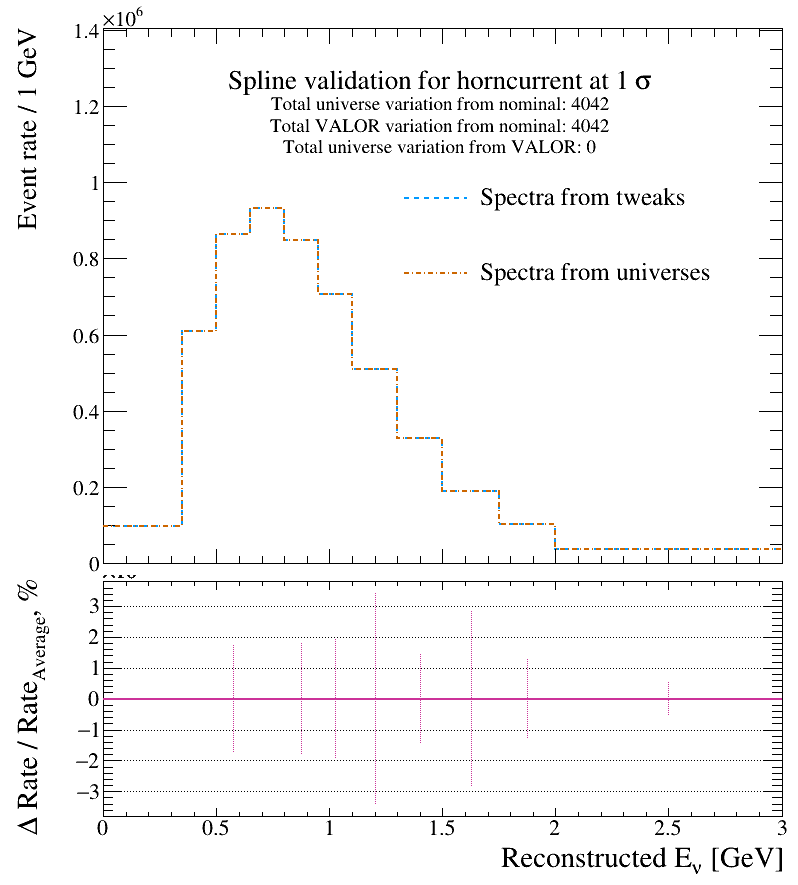
\includegraphics[width = 0.49\textwidth, height = 0.56184\textwidth]{figures-chap6/tweak_nsigma_nue/horncurrent_FluxUnisim_nuelikeCChigh_1sigma_horncurrent_FluxUnisim.png}
    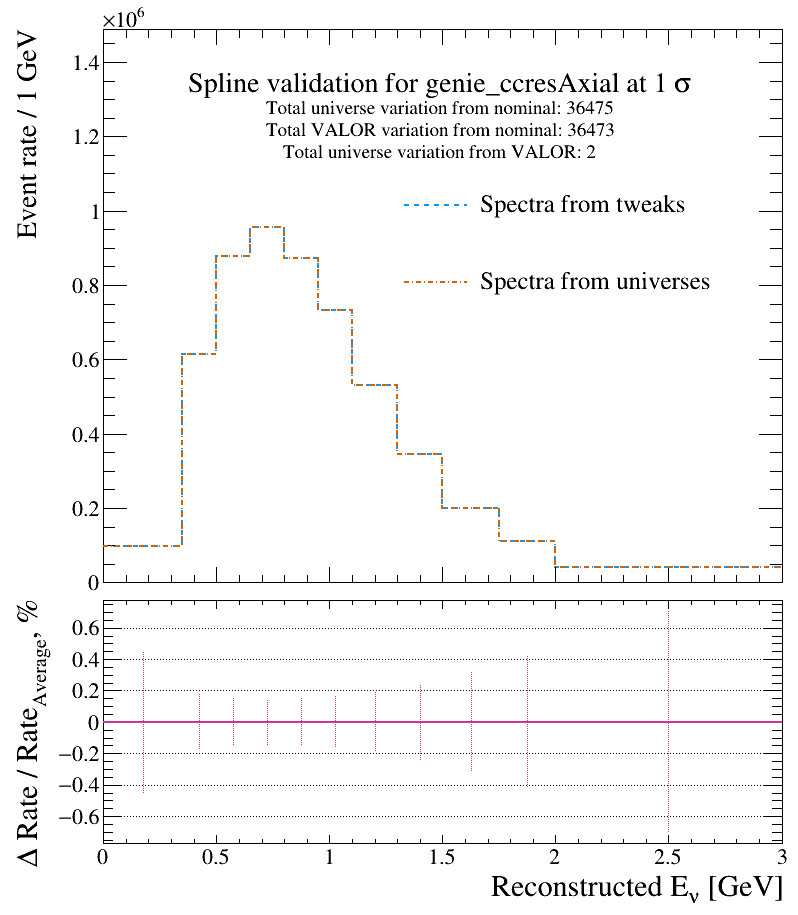
\includegraphics[width = 0.49\textwidth]{figures-chap6/tweak_nsigma_nue/genie_ccresAxial_Genie_nuelikeCChigh_1sigma_genie_ccresAxial_Genie.png}
    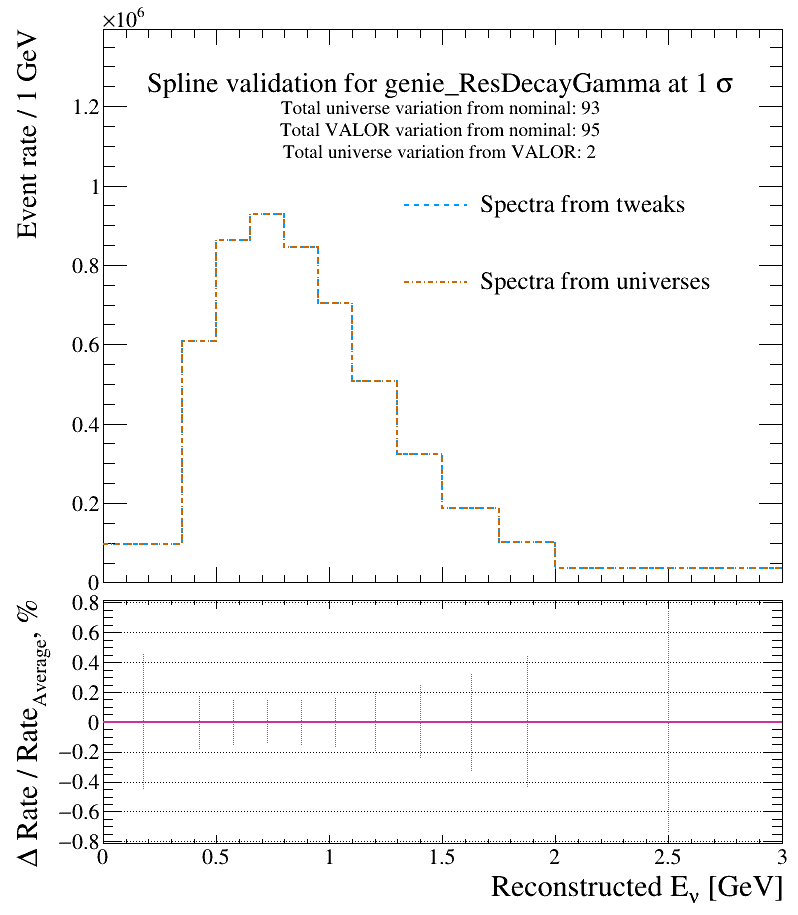
\includegraphics[width = 0.49\textwidth]{figures-chap6/tweak_nsigma_nue/genie_ResDecayGamma_Genie_nuelikeCChigh_1sigma_genie_ResDecayGamma_Genie.png}
  \captionsetup{width=0.49\textwidth}
  \parbox[b]{0.49\textwidth}%
  {
   \caption[+1$\sigma$ variation comparison for the $f_{HornCurrent}$, $f_{M_A^{CCRes}}$ and $f_{\Delta \rightarrow N \gamma}$ parameters.]{A comparison of the +1$\sigma$ variation from the response functions in VALOR and the universes for the $f_{HornCurrent}$, $f_{M_A^{CCRes}}$ and $f_{\Delta \rightarrow N \gamma}$ parameters. The $f_{HornCurrent}$ parameter shows perfect agreement between VALOR and the universes whereas both the $f_{M_A^{CCRes}}$ and $f_{\Delta \rightarrow N \gamma}$ parameters only have an event rate difference of 2. \\\phantom{.}\\
   \label{fig:+1sigma_variations}}
   }
\end{figure}

\FigureRef{fig:1sigma_variations_toys} shows a double ratio comparison from VALOR and the universes for the flux, proposal interaction and modern interaction systematic parameters. These plots are constructed by first finding the ratio between the 1$\sigma$ variation and the nominal using VALOR and the analogous ratio using the universe files. The double ratio is then constructed by taking the ratio of both the previous 1$\sigma$ ratios. There are some minor differences between the variation in VALOR and the universes, however, event perfect agreement isn't expected since the 1$\sigma$ variations are found by taking the average from many toy samples. Nevertheless, the disagreement is for the most part $< 1\%$ with a maximum of just over 2\%. 



\begin{figure}[h!]
    \begin{comment}
    Was too lazy to remake the plots and remove the label so have just overlayed a white box to hide.
    \end{comment}
    \begin{tikzpicture}
    \node at (0,0) {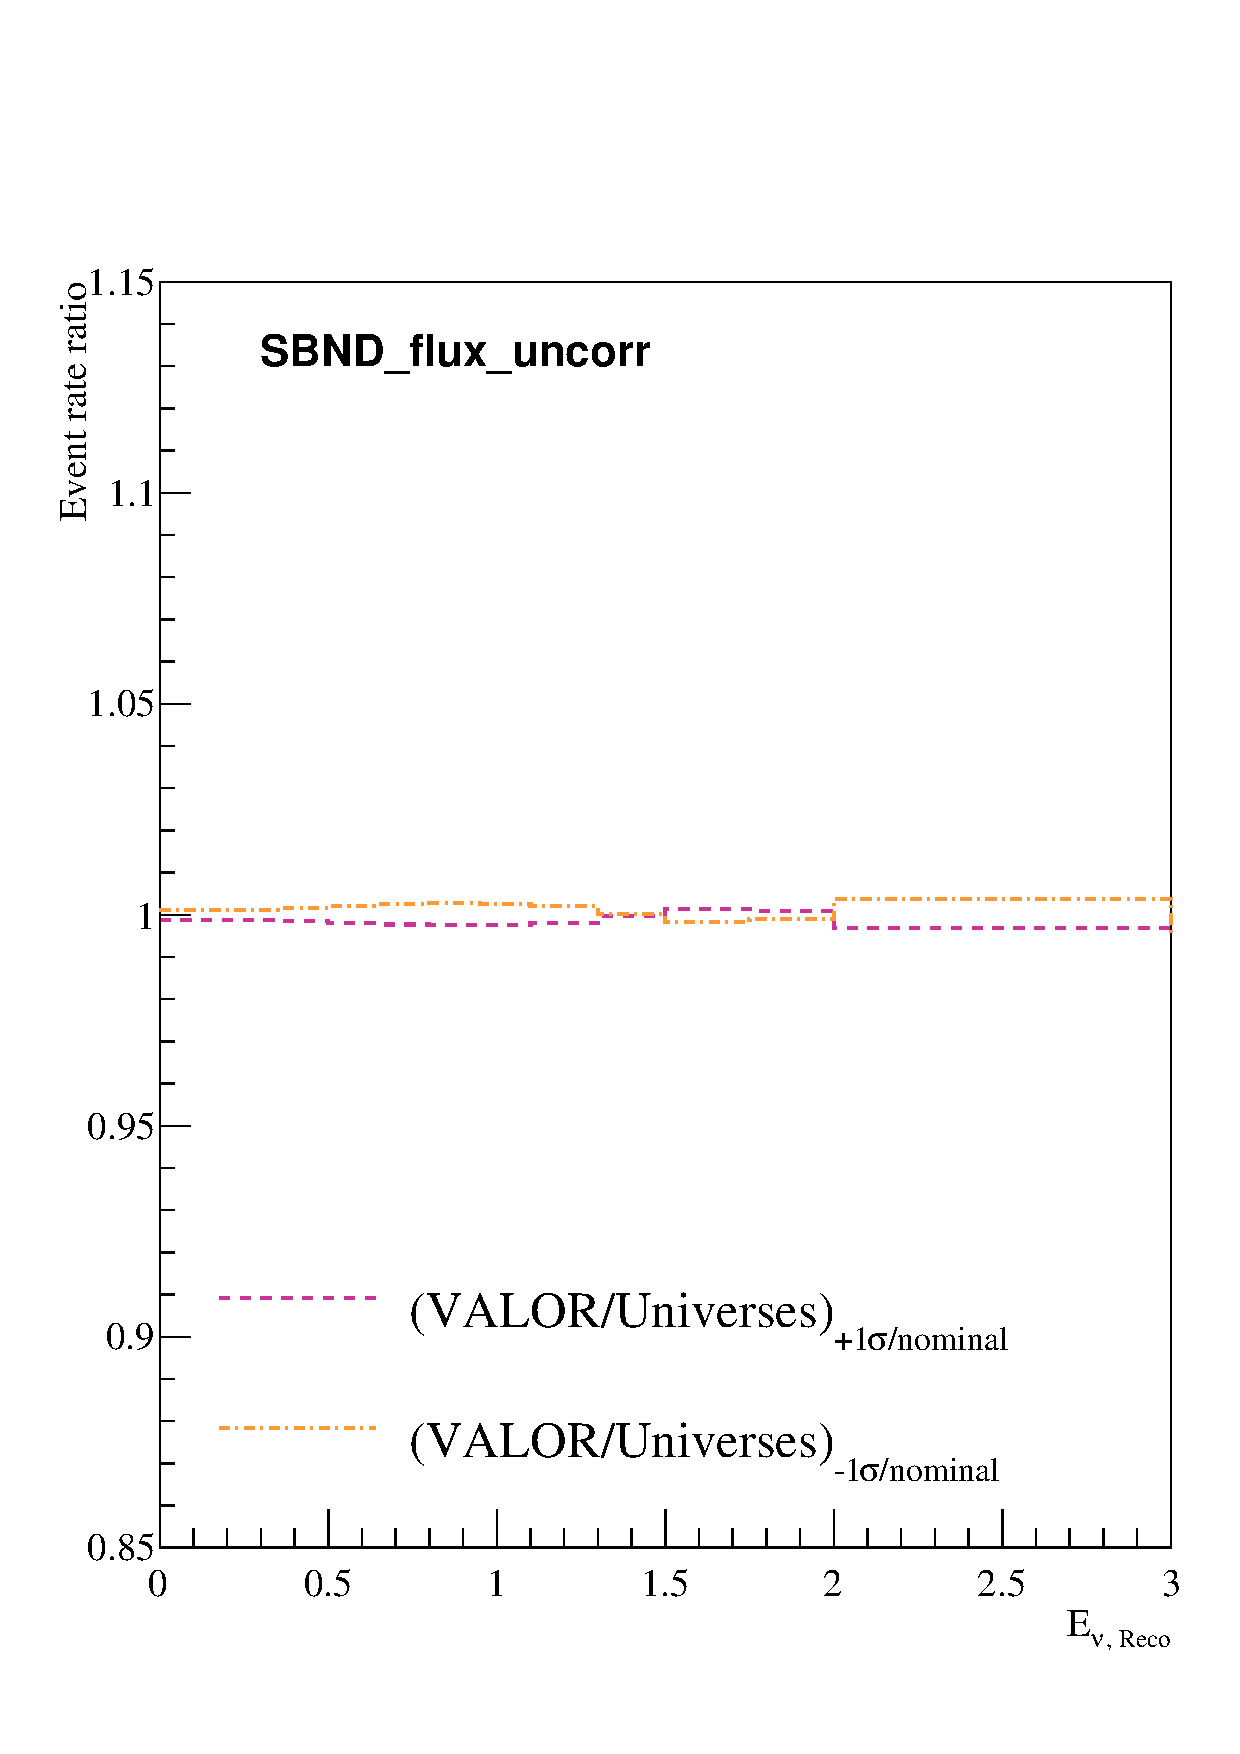
\includegraphics[width = 0.45\textwidth, height = 0.56184\textwidth]{figures-chap6/tweak_pdf_N_nue/universe_valor_double_ratios_SBND_flux_uncorr.pdf}};
    \draw [fill=white, draw=white] (-2.5,3)--(1,3)--(1,3.5)--(-2.5,3.5)--cycle;
    \end{tikzpicture}
    %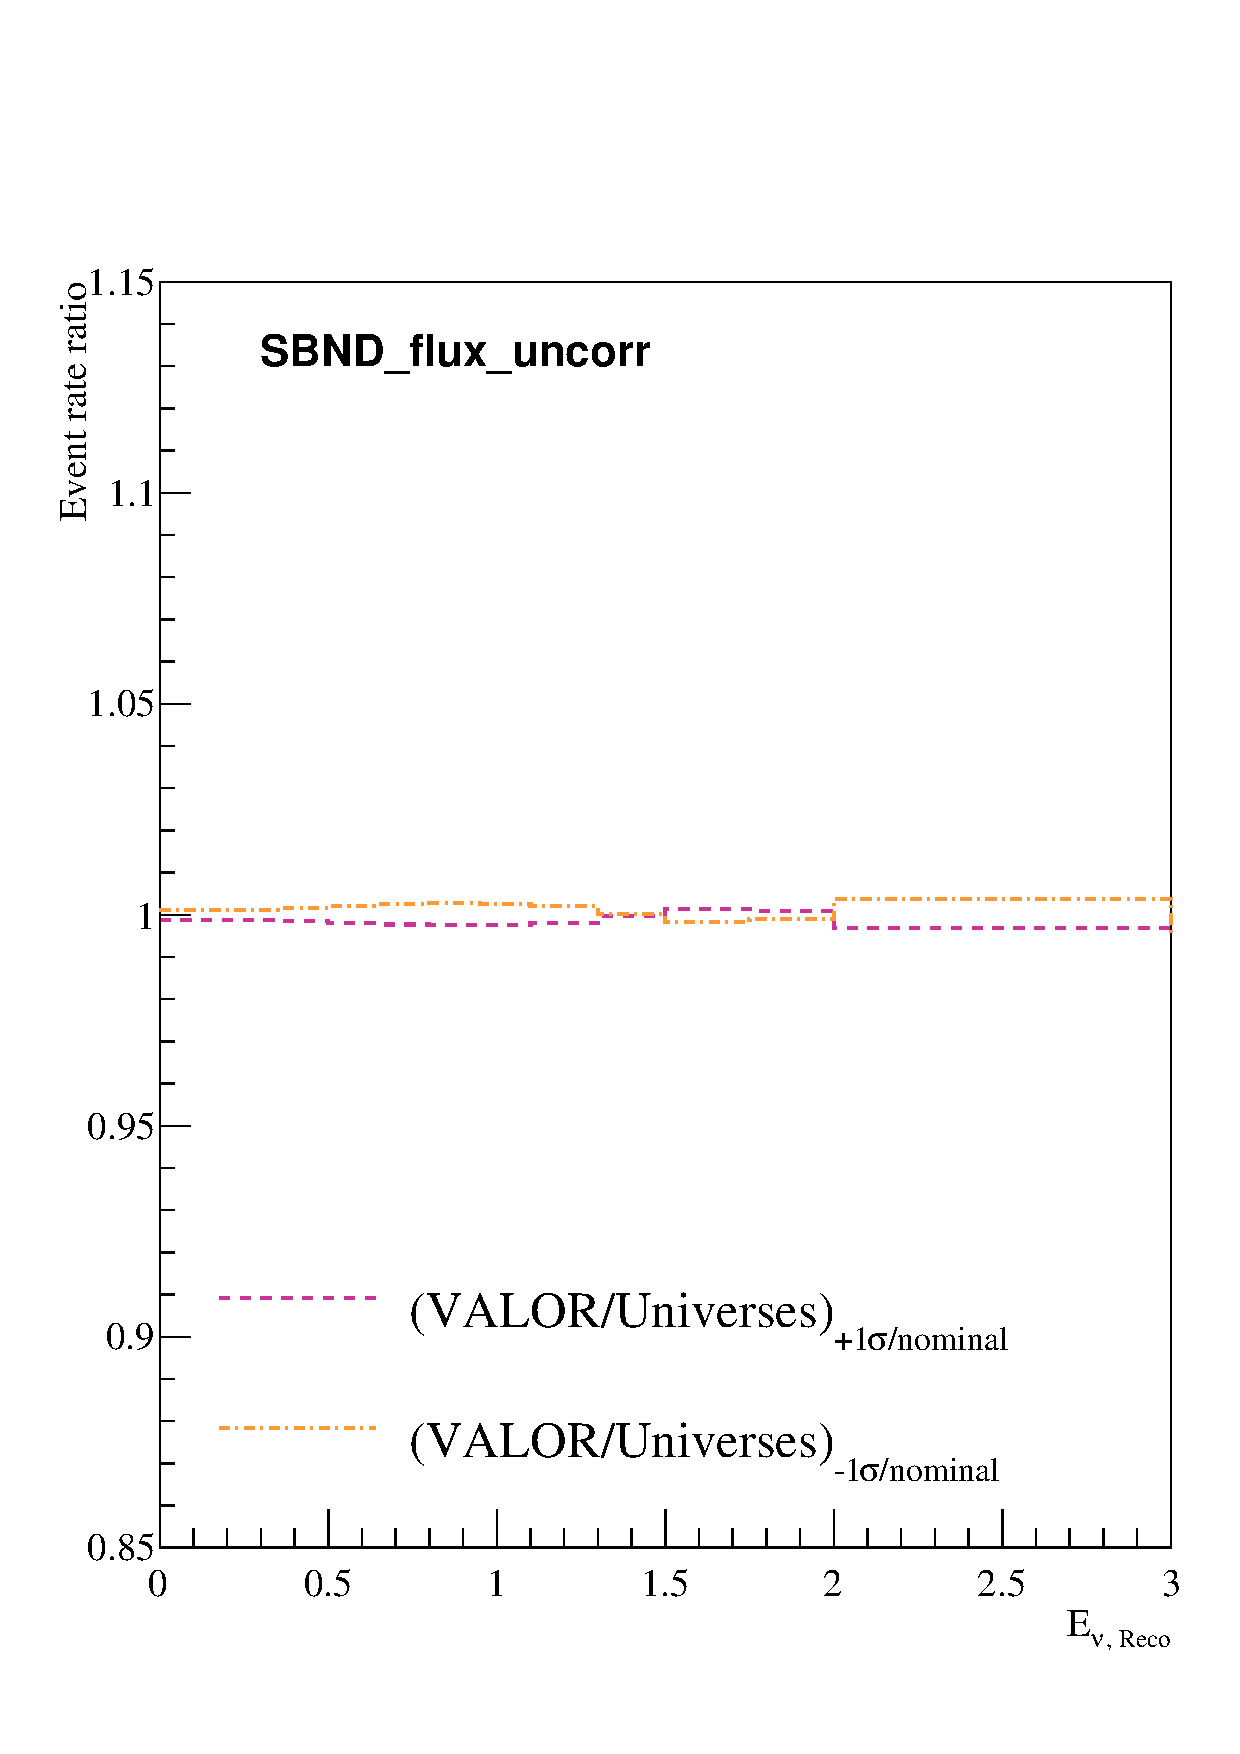
\includegraphics[width = 0.49\textwidth, height = 0.56184\textwidth]{figures-chap6/tweak_pdf_N_nue/universe_valor_double_ratios_SBND_flux_uncorr.pdf}
    \begin{tikzpicture}
    \node at (0,0) {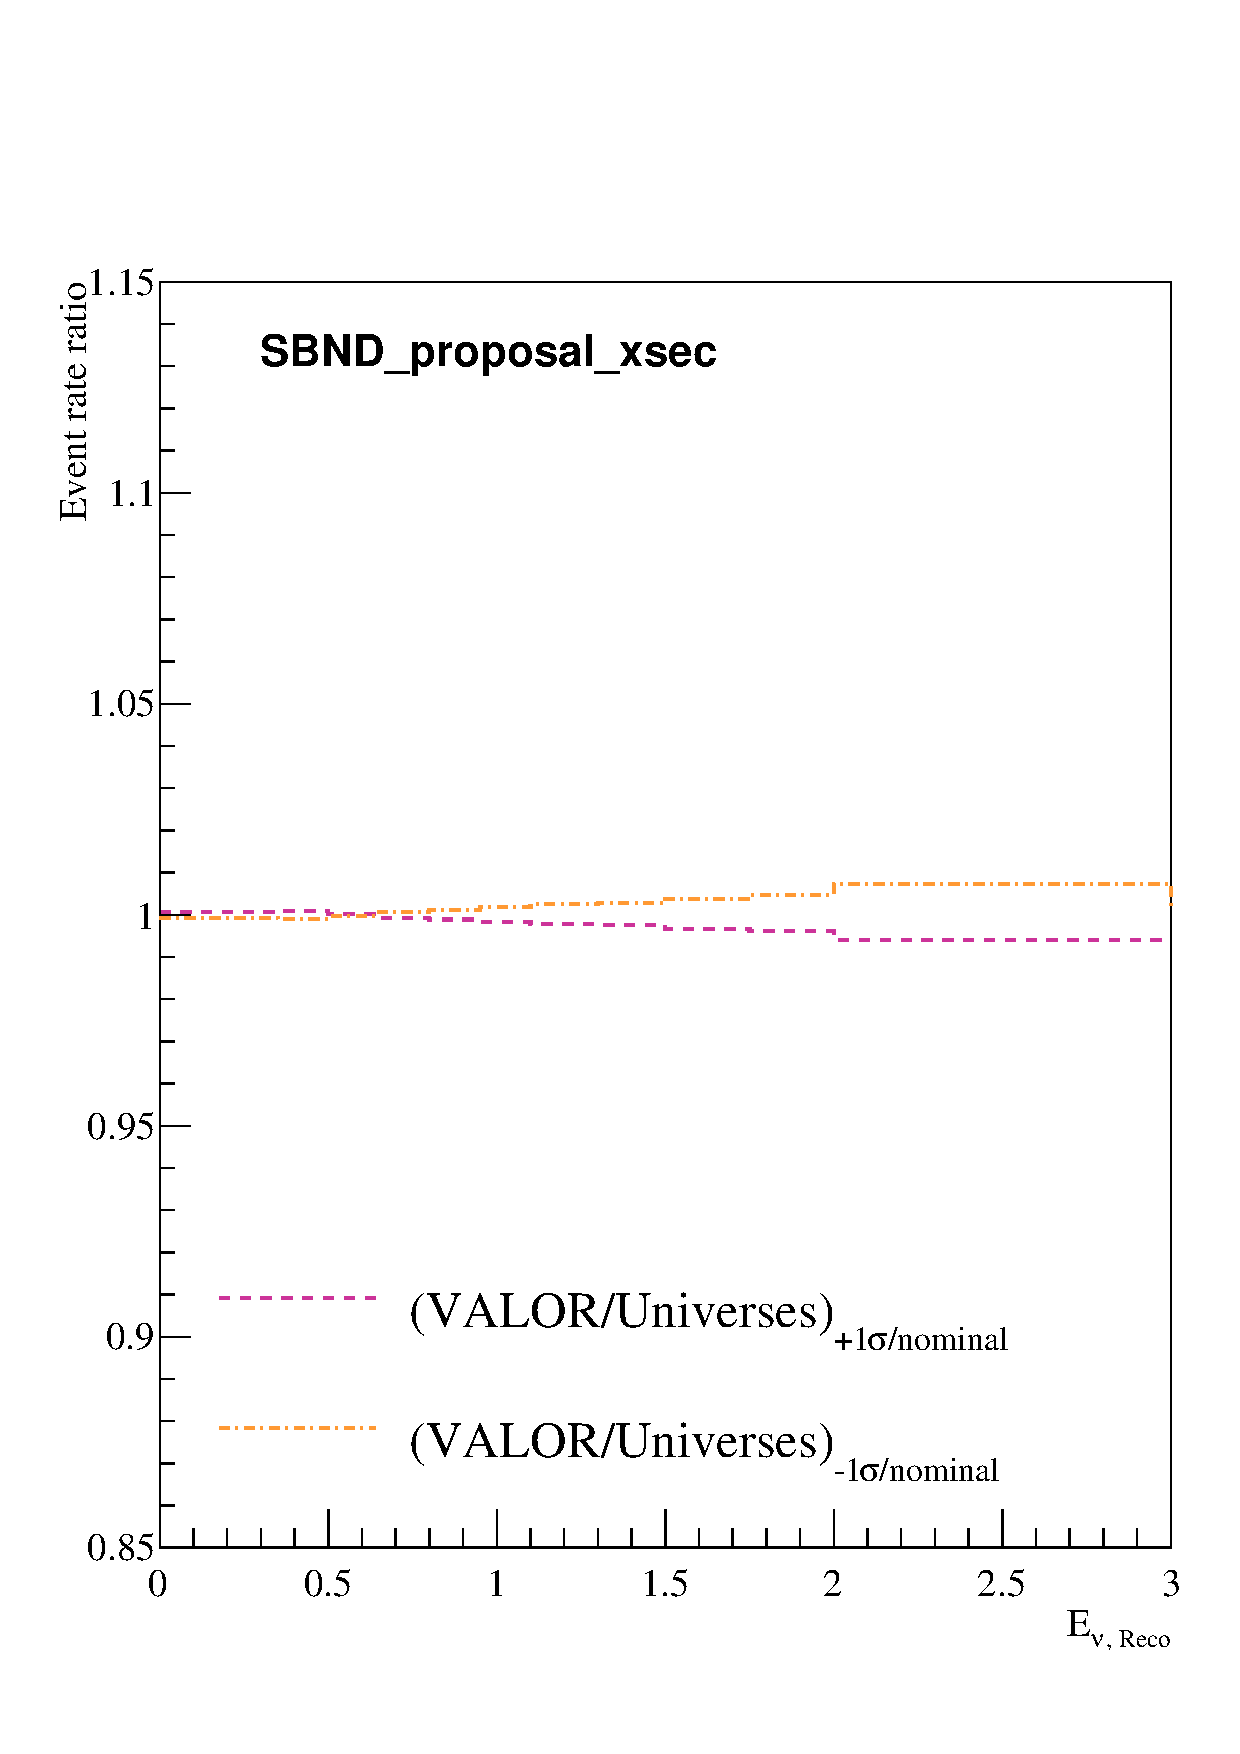
\includegraphics[width = 0.45\textwidth, height = 0.56184\textwidth]{figures-chap6/tweak_pdf_N_nue/universe_valor_double_ratios_SBND_proposal_xsec.pdf}};
     \draw [fill=white, draw=white] (-2.5,3)--(1,3)--(1,3.5)--(-2.5,3.5)--cycle;
    \end{tikzpicture}
    \begin{tikzpicture}
    \node at (0,0) {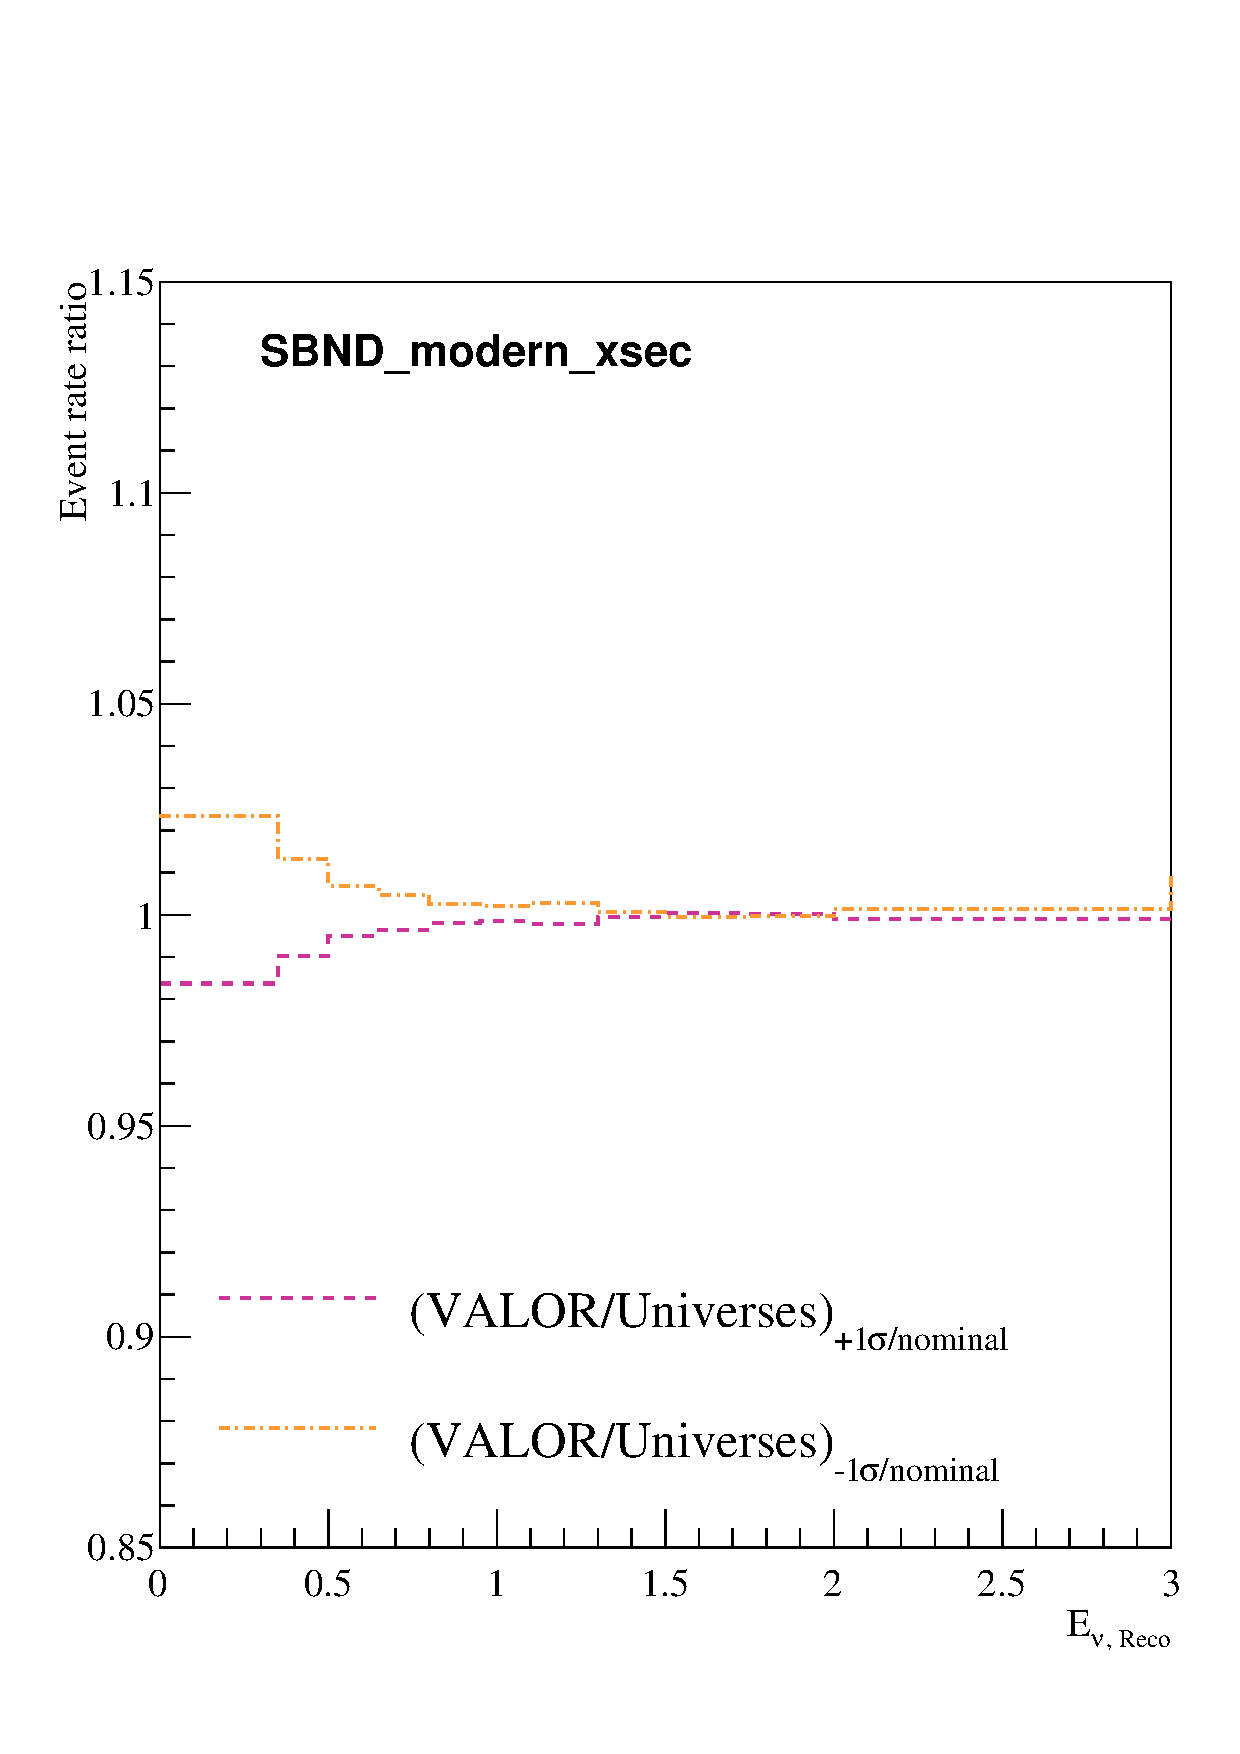
\includegraphics[width = 0.45\textwidth, height = 0.56184\textwidth]{figures-chap6/tweak_pdf_N_nue/universe_valor_double_ratios_SBND_modern_xsec.pdf}};
     \draw [fill=white, draw=white] (-2.5,3)--(1,3)--(1,3.5)--(-2.5,3.5)--cycle;
    \end{tikzpicture}
    \vspace{0.1\textwidth}
  \captionsetup{width=0.45\textwidth}
  \parbox[b]{0.45\textwidth}%
  {
   \caption[The ratio between the $\pm 1 \sigma$ variation from VALOR. and the universes for the flux, proposal interaction and modern interaction set of systematics.]{The ratio between the $\pm 1 \sigma$ variation from VALOR and the universes for the flux, proposal interaction and modern interaction set of systematic parameters.  \\\phantom{.}\\\phantom{.}\\\phantom{.}\\
   \label{fig:1sigma_variations_toys}}
  }
\end{figure}

\clearpage
\subsection{Impact of systematic uncertainties}

\textcolor{red}{Not sure where best to put this section? Here or along with the sensitivity curves.}

To assess the impact of the different systematic parameters on the oscillation parameters the following study is performed;
\begin{enumerate}
    \item Generate a toy experiment with a given oscillation signal with a single systematic parameter, $f_i$, set to $\pm1\sigma$ from it's nominal value and all other systematic parameters are set to their nominal value.
    \item Perform a fit on the toy experiment with $f_i$ fixed to its nominal value. Both the oscillation parameters and all the systematic parameters are initially set to their nominal value and are allowed to float with the exception of $f_i$. The other systematic parameters are allowed to float in order to obtain the best possible agreement between the fit and the toy experiment.
    \item Steps 1. and 2. are then repeated for all \textit{i} systematic parameters of interest. Both the +1$\sigma$ and -1$\sigma$ variations should be performed for each systematic parameter since the effect on the oscillation parameters is typically not symmetric.  
\end{enumerate}
If $f_i$ were allowed to float it would be expected that the fit would be able to recover the same oscillation parameters used in the toy experiment since the same \gls{mc} was used for the toy experiment and the fit. By fixing $f_i$ to its nominal value in the fit, the fit is forced to make a mistake. This results in the fit remapping the changes in $f_i$ to the oscillation parameters (and the other systematic parameters). 

This study was performed for the \nue appearance and disappearance channels using oscillation parameters $\sin^2{2\theta}_{\mu e} = 0.003$, 
$\Delta m^2_{41} = 1.32$ eV$^2$ and 
$\sin^2{2\theta}_{ee} = 0.4$, $\Delta m^2_{41} = 3$ eV$^2$ respectively and includes the results from all uncorrelated systematic parameters. The results are shown in \FigureRef{fig:nue_app_osc_param_pulls} and \FigureRef{fig:nue_disapp_osc_param_pulls}. For both oscillation parameters, the ratio of their value after performing the fit to their nominal value, $\mathcal{R}$, are shown after having varied $f_i$ by $\pm 1 \sigma$. The ratios shown in \FigureRef{fig:nue_app_osc_param_pulls} and \FigureRef{fig:nue_disapp_osc_param_pulls} are always $\geq 1$ by construction since $\mathcal{R}$ is defined as,
\begin{equation}
    \mathcal{R} = \begin{cases}
    \frac{\zeta_{fit}}{\zeta_{nom}}, & \text{if } \zeta_{fit} > \zeta_{nom} \\
    \frac{\zeta_{nom}}{\zeta_{fit}}, &\text{if } \zeta_{nom} > \zeta_{fit},
    \end{cases}
\end{equation}
where $\zeta \in \{\sin^2{2\theta}, \Delta m^2_{41}\}$ and the subscript \textit{nom} and \textit{fit} refer to the nominal value of the oscillation parameters and the values after performing the fit respectively. The arrows are colour coded such that black corresponds to the case where $\zeta_{fit} > \zeta_{nom}$ and red corresponds to the case where $\zeta_{nom} > \zeta_{fit}$.

\begin{figure}[h!]
    \centering
    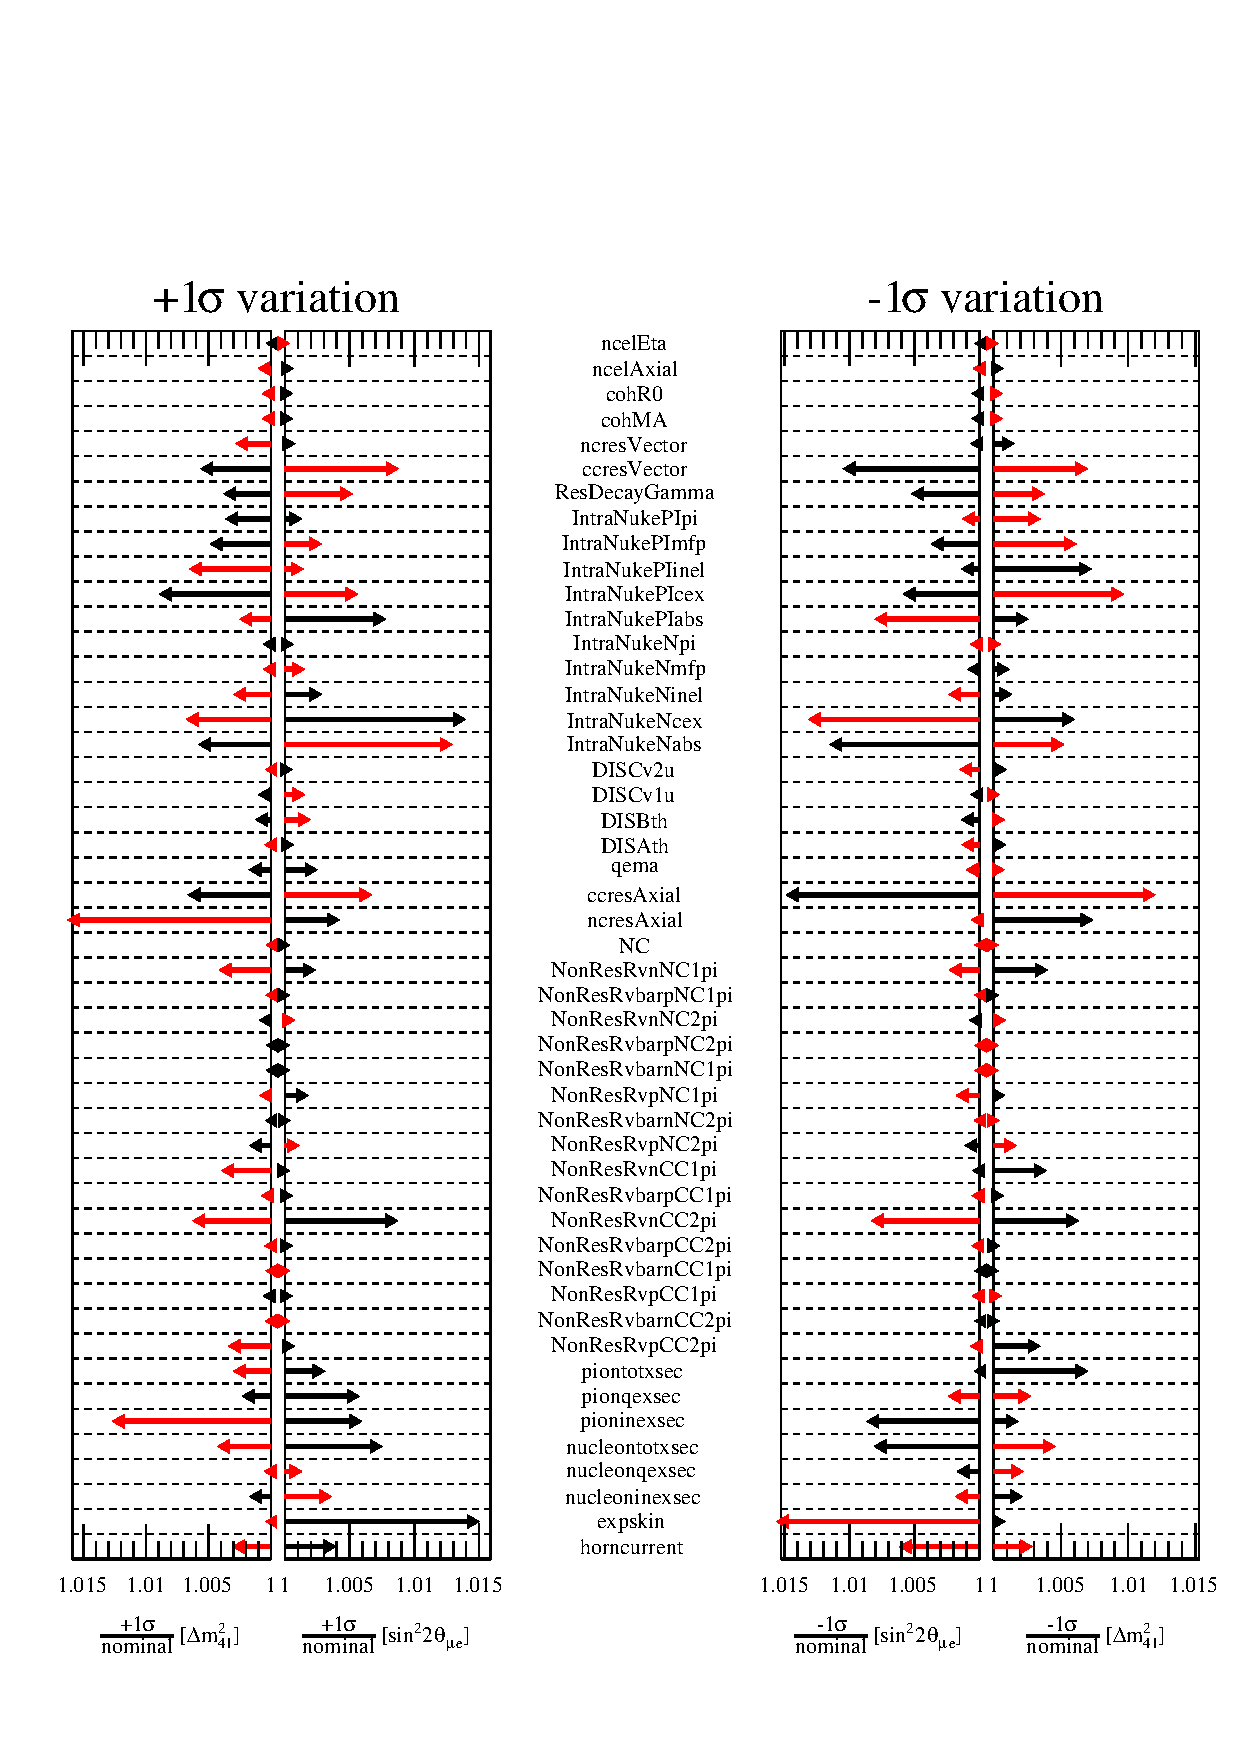
\includegraphics[width = \largefigwidth]{figures-chap6/star_plot/nue_app_pulls.pdf}
    \caption[\nue appearance oscillation parameter pulls due to varying a single systematic parameter by $\pm1\sigma$.]{The variation in the \nue appearance oscillation parameters due to varying a single systematic parameter at a time by $\pm1\sigma$.}
    \label{fig:nue_app_osc_param_pulls}
\end{figure}

\begin{figure}[h!]
    \centering
    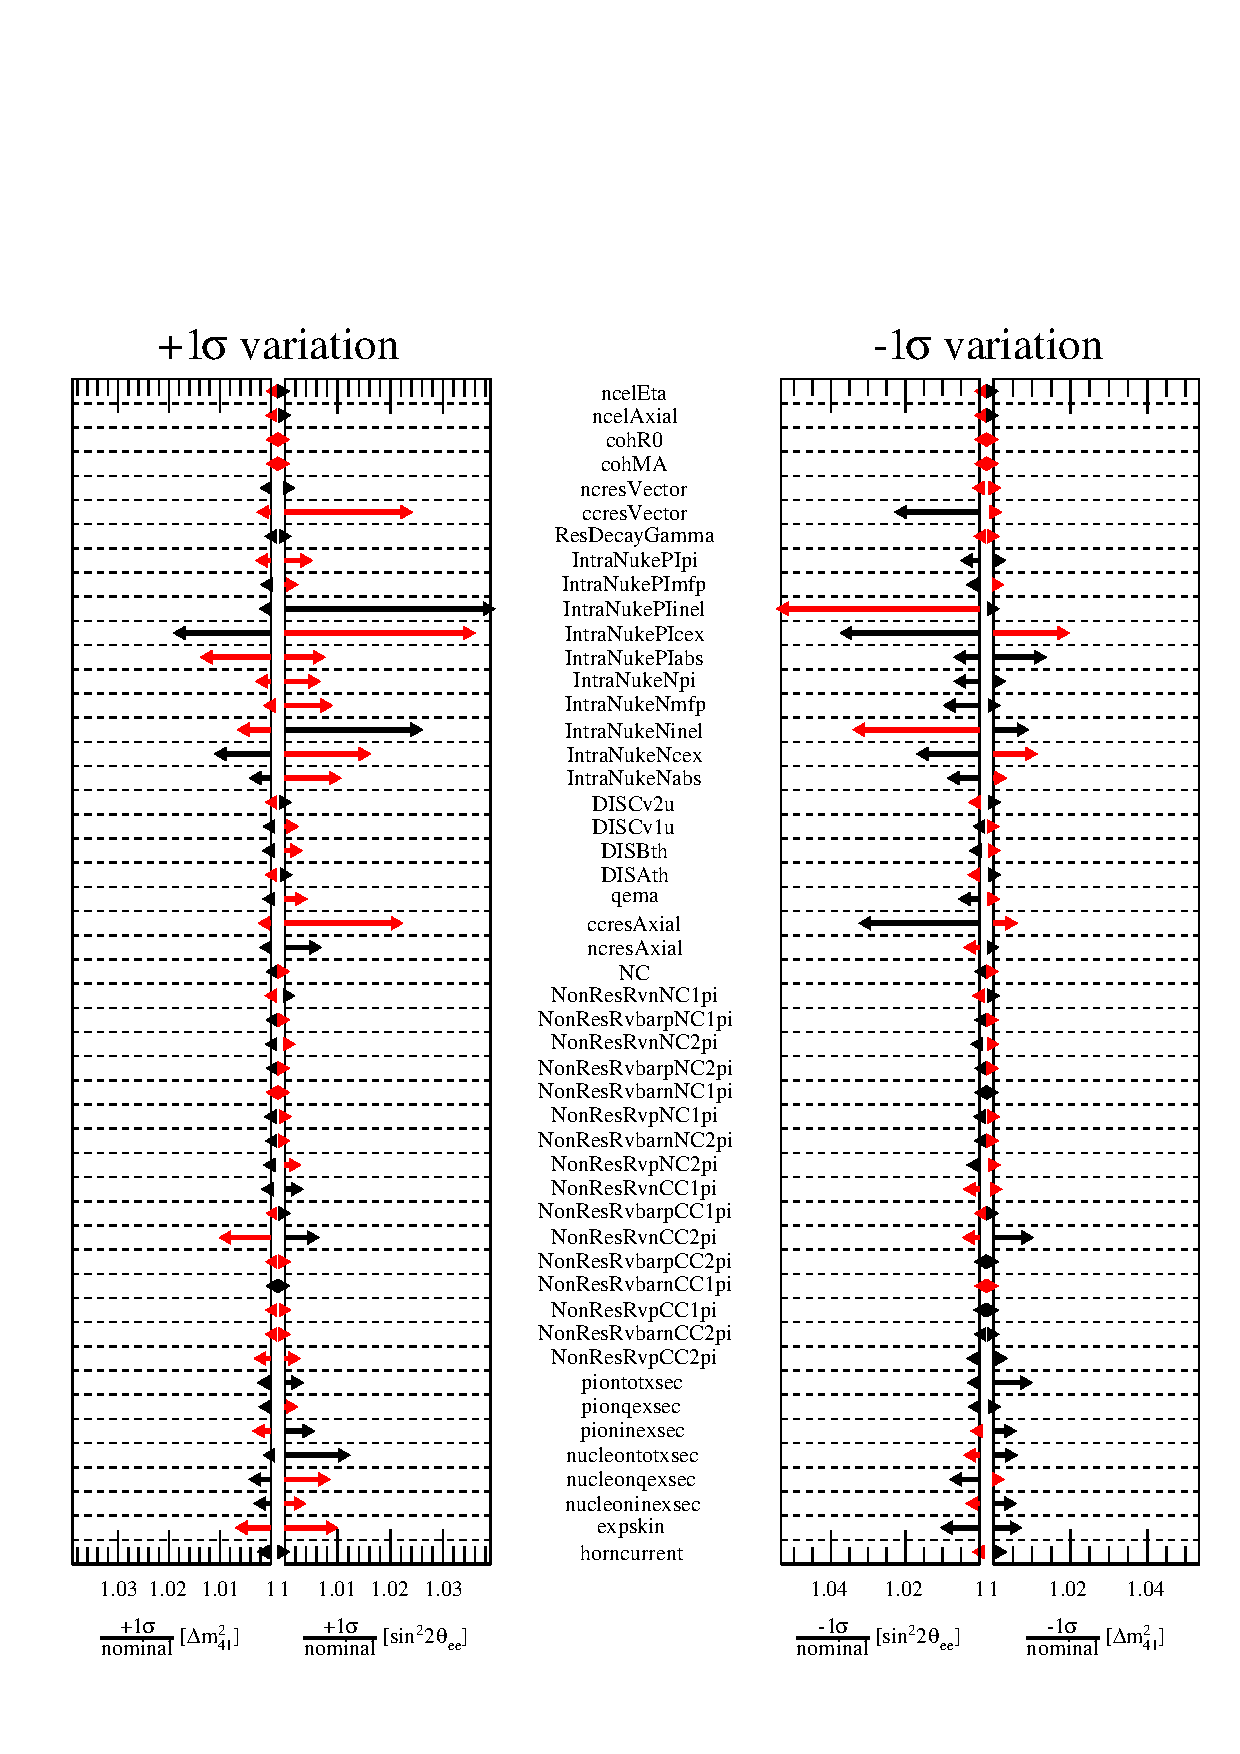
\includegraphics[width = \largefigwidth]{figures-chap6/star_plot/nue_dsisapp_pulls.pdf}
    \caption[\nue disappearance oscillation parameter pulls due to varying a single systematic parameter by $\pm1\sigma$.]{The variation in the \nue disappearance oscillation parameters due to varying a single systematic parameter at a time by $\pm1\sigma$.}
    \label{fig:nue_disapp_osc_param_pulls}
\end{figure}

The impact of the $f_{M_V^{CCRes}}$, $f_{M_A^{CCRes}}$, $f_{R_N^{C Ex}}$ and $f_{\sigma^{\pi}_{INEL}}$ parameter on the \nue appearance exclusion sensitivities are shown in \FigureRef{fig:nue_app_single_param}. The parameters were applied one at a time and chosen as some that showed the largest variations in \FigureRef{fig:nue_app_osc_param_pulls}, ensuring at least on parameter from each systematic subgroup. Similarly, the $f_{M_V^{CCRes}}$, $f_{M_A^{CCRes}}$, $f_{R_{\pi}^{C Ex}}$ and $f_{expskin}$ parameters were used for the \nue disappearance channel and the results are shown in \FigureRef{fig::nue_disapp_single_param}.

\begin{figure}[h!]
    \centering
    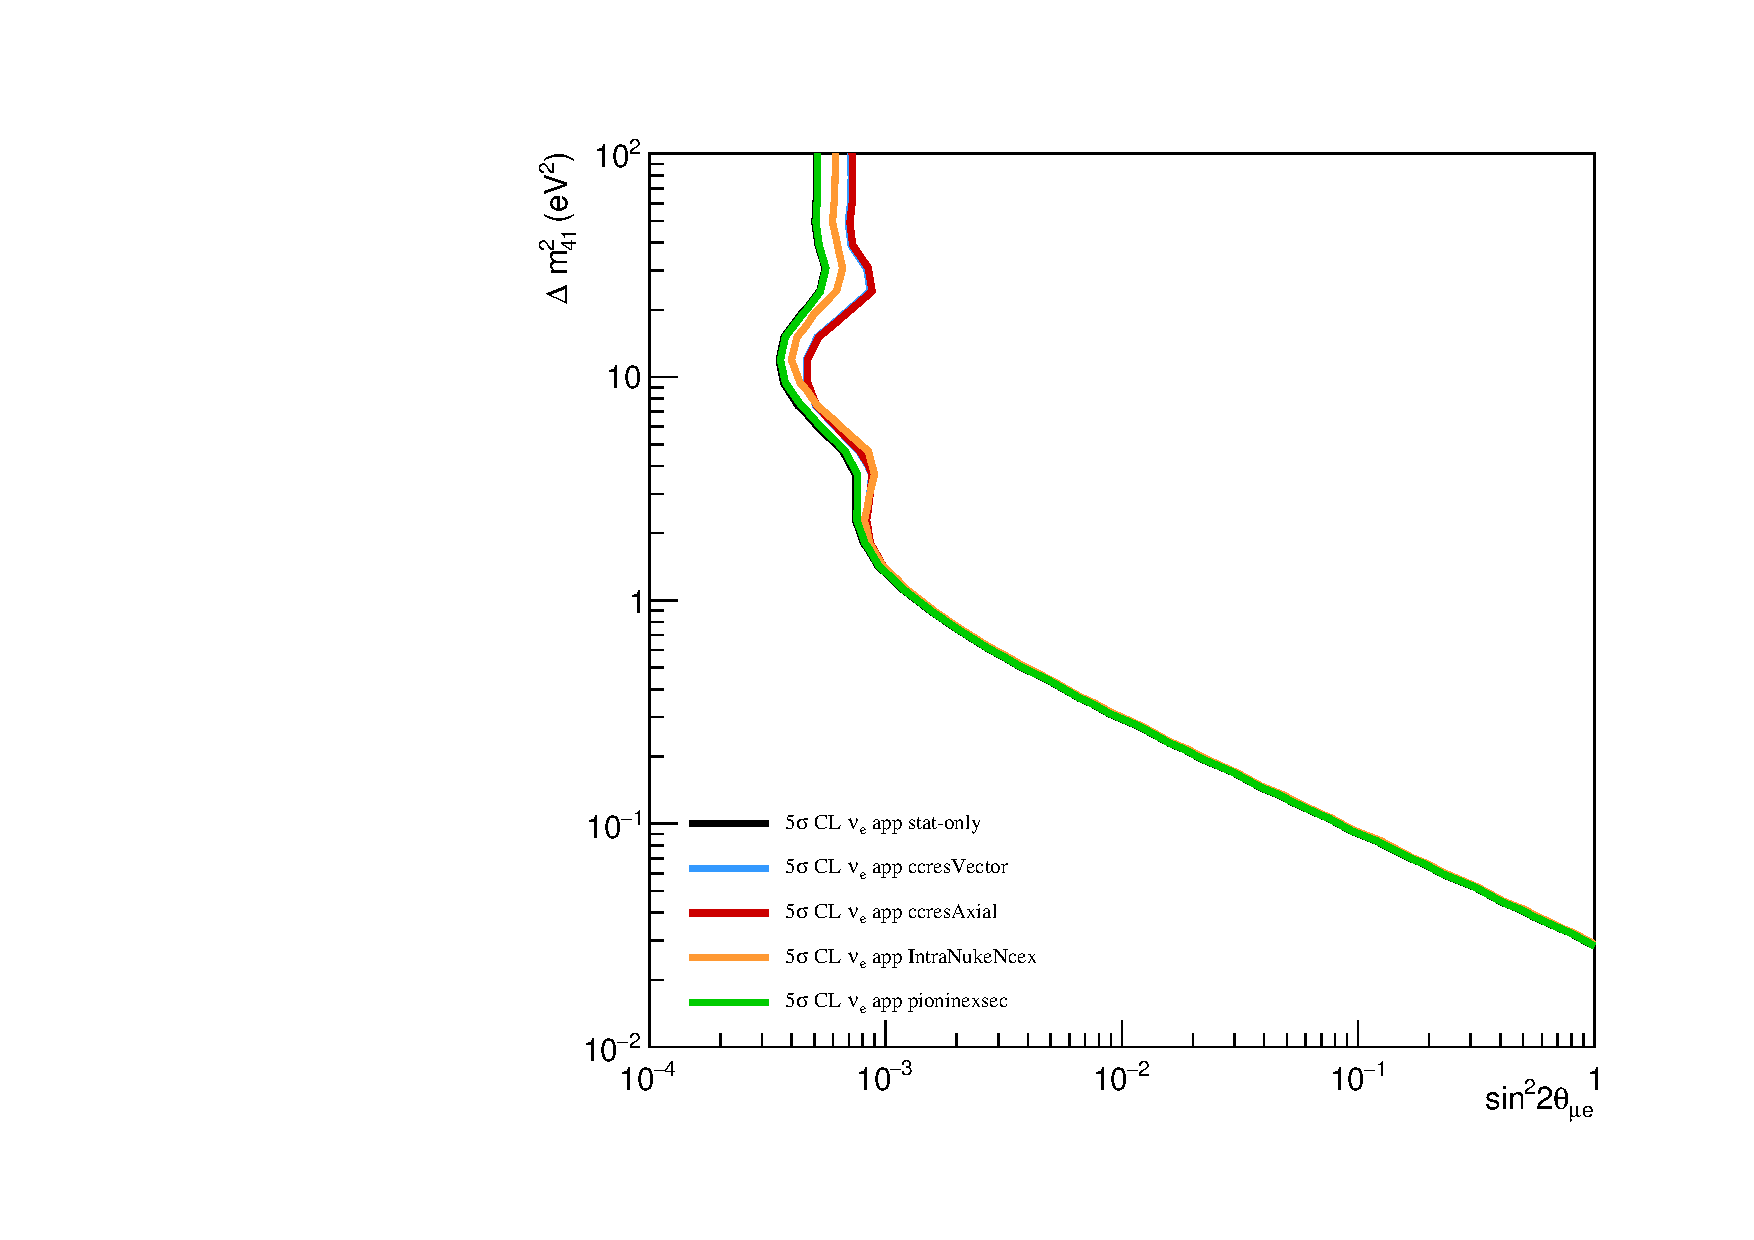
\includegraphics[width = 0.49\textwidth]{figures-chap6/exclusion_contours/single_param/nue_app_single_param.pdf}
    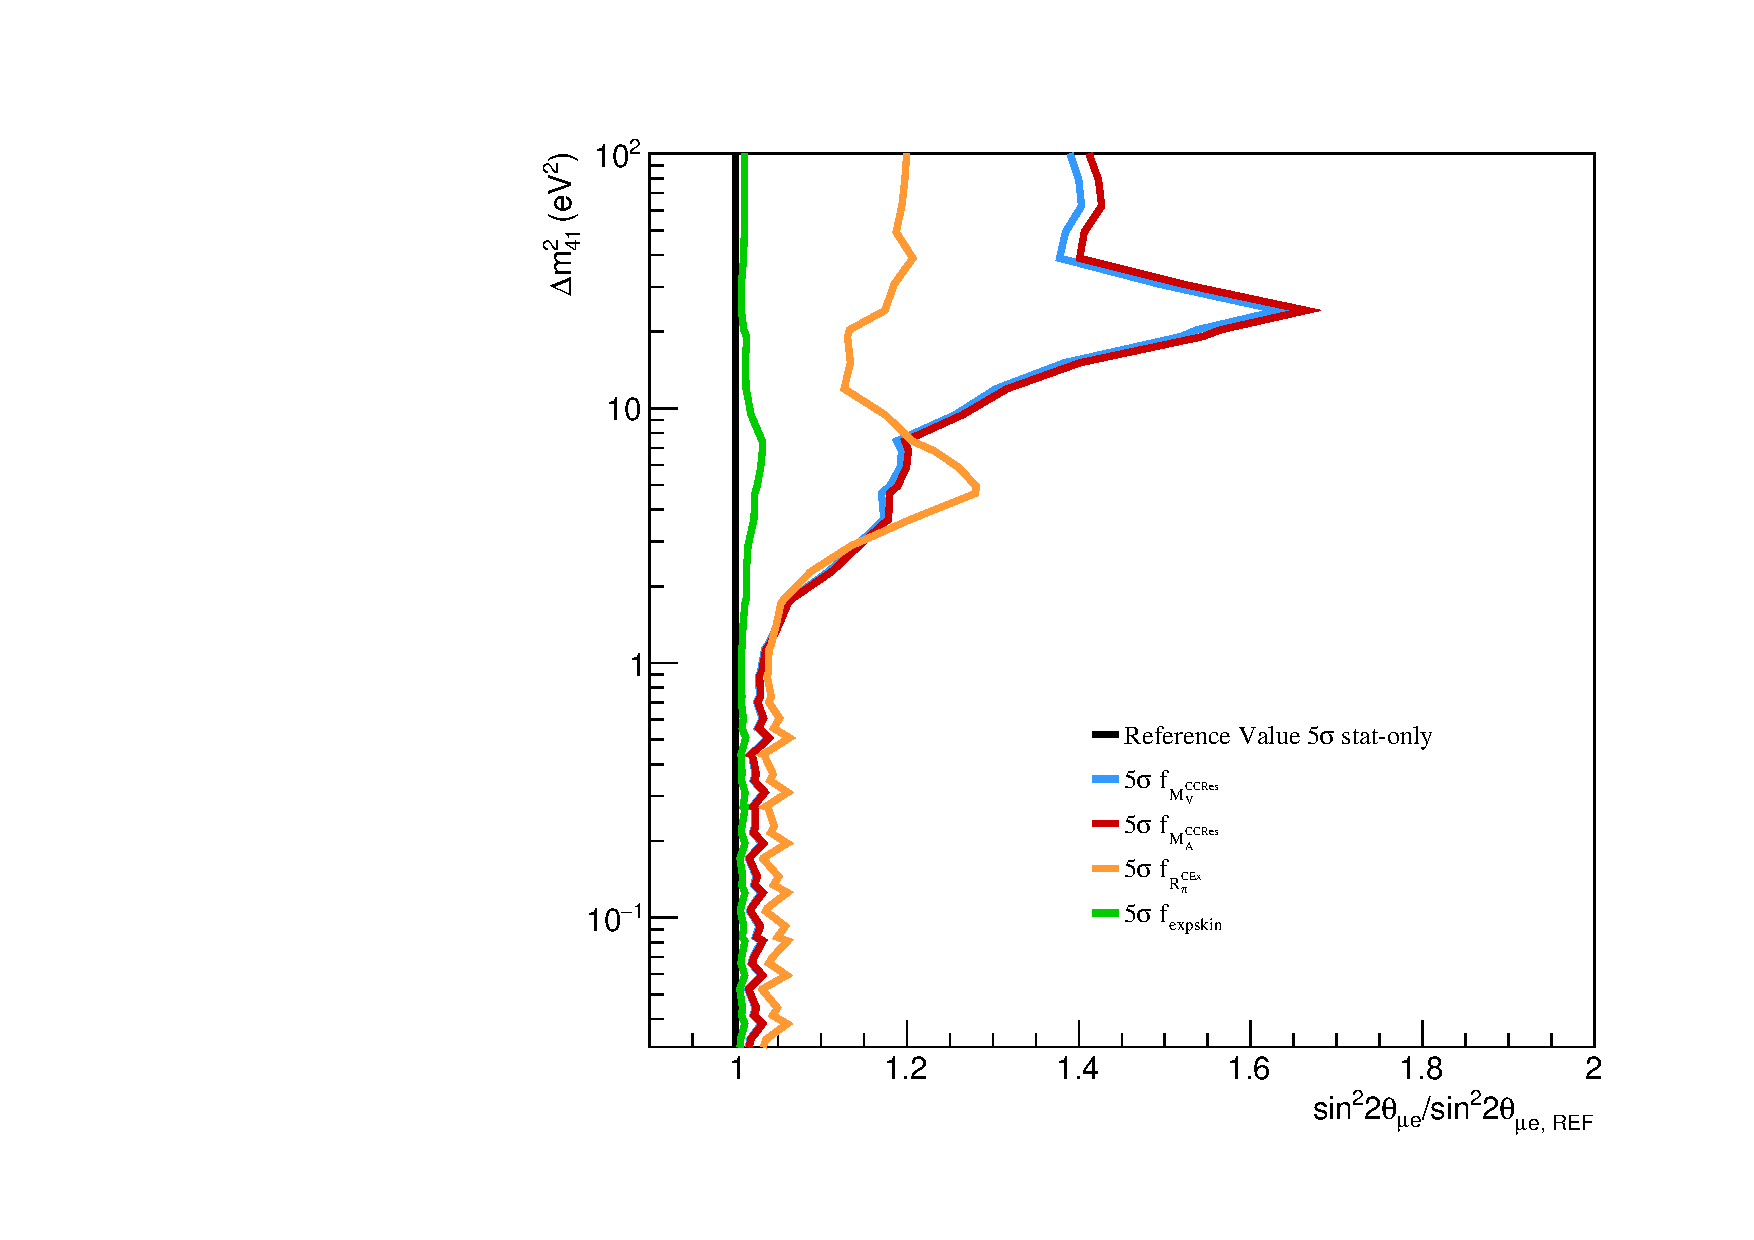
\includegraphics[width =0.49\textwidth]{figures-chap6/exclusion_contours/single_param/nue_app_single_param_ratio.pdf}
    \caption[\nue appearance exclusion contours with inclusion of a single systematic parameter at a time.]{Left: \nue appearance exclusion contours with inclusion of a single systematic parameter at a time. The systematic parameters considered are ccresVector, ccresAxial, IntraNukeNcex and pioninexsec. Right: The ratio of the exclusion contours with the inclusion of a systematic parameter the statistical only contour.}
    \label{fig:nue_app_single_param}
\end{figure}

\begin{figure}[h!]
    \centering
    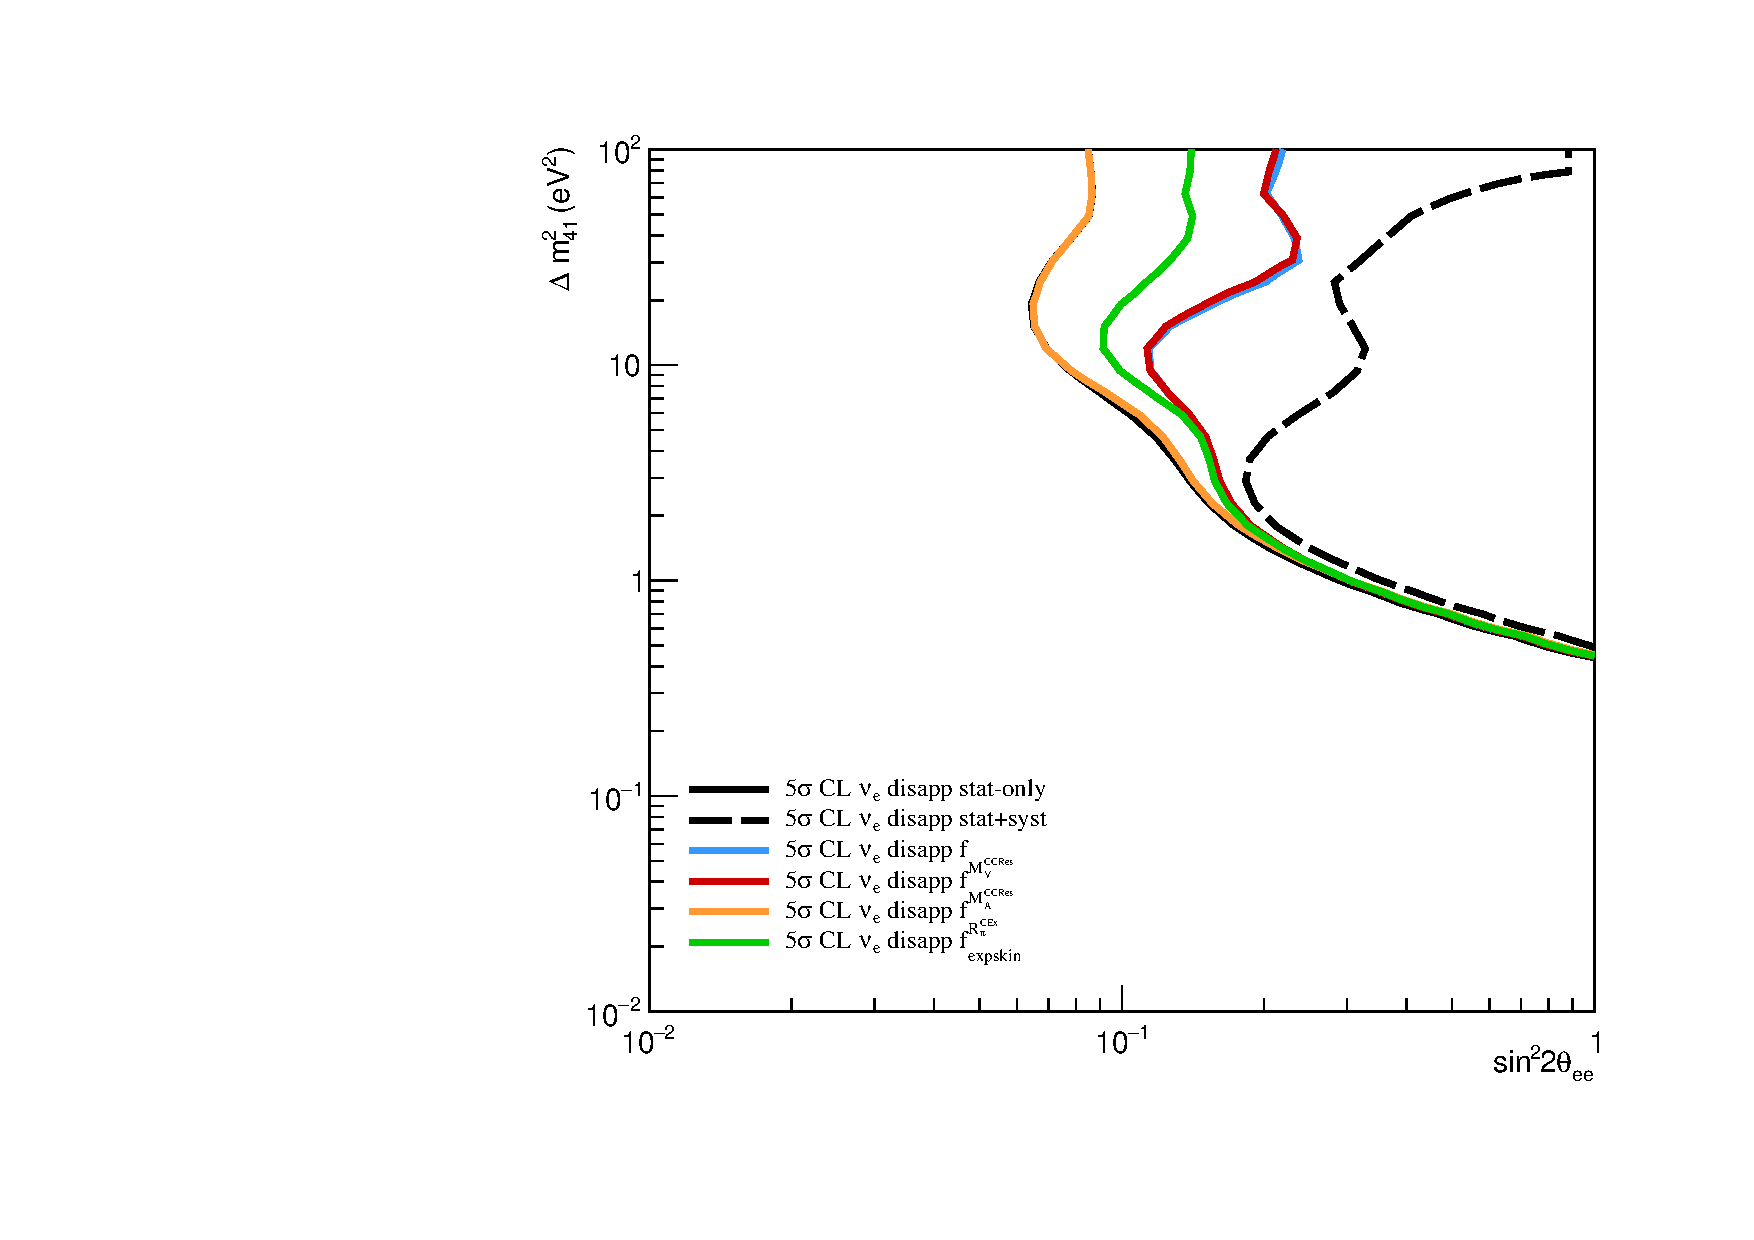
\includegraphics[width = 0.49\textwidth]{figures-chap6/exclusion_contours/single_param/nue_disapp_single_param.pdf}
    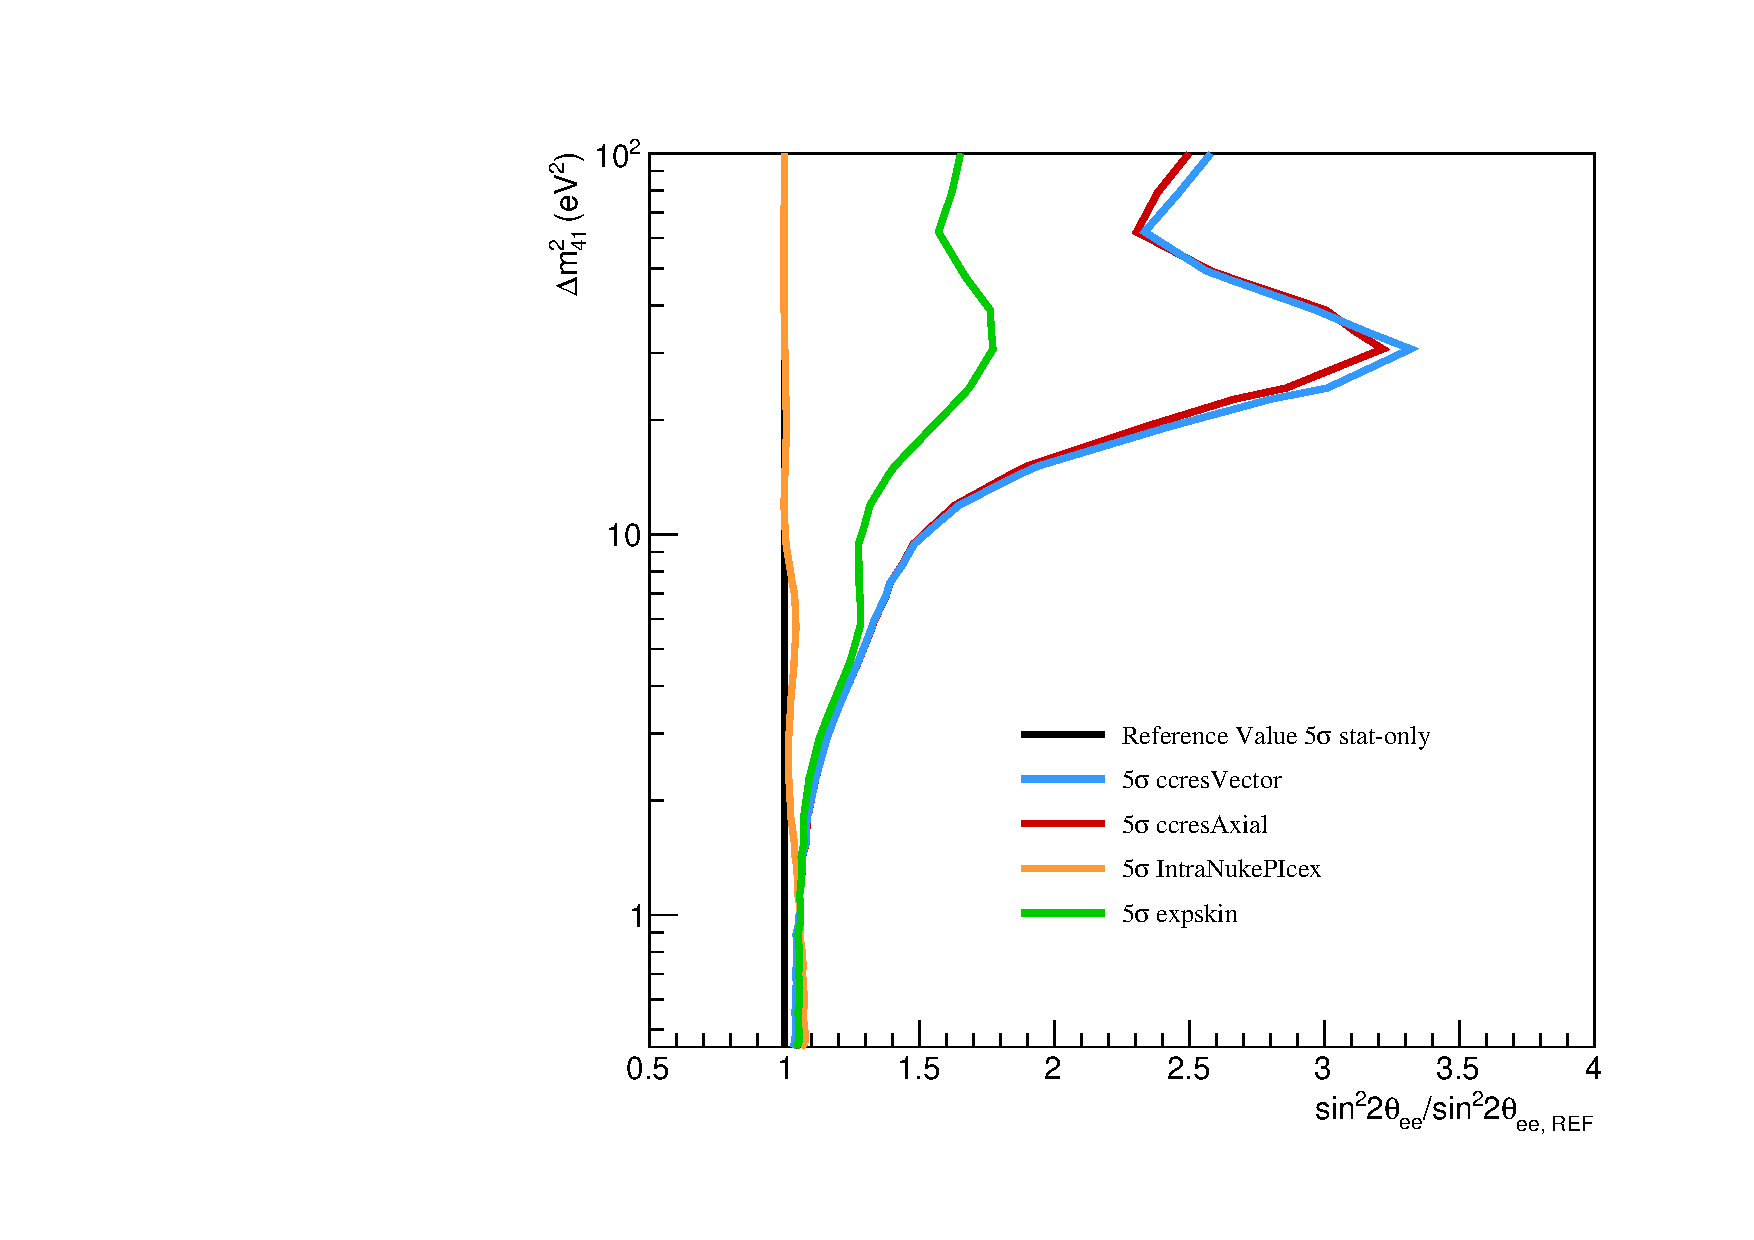
\includegraphics[width =0.49\textwidth]{figures-chap6/exclusion_contours/single_param/nue_disapp_single_param_ratio.pdf}
    \caption[\nue disappearance exclusion contours with inclusion of a single systematic parameter at a time.]{Left: \nue disappearance exclusion contours with inclusion of a single systematic parameter at a time. The systematic parameters considered are ccresVector, ccresAxial, IntraNukeNcex and pioninexsec. Right: The ratio of the exclusion contours with the inclusion of a systematic parameter the statistical only contour.}
    \label{fig::nue_disapp_single_param}
\end{figure}
\clearpage
\section{\texorpdfstring{$\nue$ Analysis}{nue Analysis}}\label{sec:nue_analysis}

As was mentioned in \SectionRef{sec:sterile_neutrino_oscillations}, there are two oscillations channels associated with \nue; \nue appearance and \nue disappearance. Since the only difference between these channels is due to oscillations, the nominal event rates are common between the two. 

The breakdown of the nominal number of events by interaction mode and channel is shown numerically in \TableRef{table:sbnd_nue_event_rate}, \TableRef{table:uboone_nue_event_rate} and \TableRef{table:icarus_nue_event_rate} for \gls{sbnd}, \gls{microboone} and \gls{icarus} respectively. The same events rates are also shown in \FigureRef{fig:nominal_nue_spectra} in the form of spectra. The spectra show the modal breakdown in terms of the coarse reaction modes where the events have been binned in reconstructed neutrino energy. 

Similar to \FigureRef{fig:nominal_nue_spectra}, \FigureRef{fig:nominal_nue_spectra_1sigma_enevelope} again shows the nominal event rate in each \gls{sbn} detector, but in an integrated form. Additionally, $1\sigma$ prefit uncertainty envelopes are shown which are due to the flux and interaction systematics. The accuracy of say the \gls{icarus} prediction can be improved by constraining the systematics from an \gls{sbnd} fit. This is shown in \FigureRef{fig:icarus_pre_post_fit} which shows the nominal integrated \gls{icarus} spectrum along with the prefit uncertainty envelope as in \FigureRef{fig:nominal_nue_spectra_1sigma_enevelope}, but also a postfit uncertainty envelope based on an \gls{sbnd} fit is shown. The reduction in size from the prefit to postfit envelope highlights the impact of \gls{sbnd} on the \gls{icarus} prediction. 

\newpage
\begin{table}
%\section*{sbn\_nd\_\_BNB\_FHC\_\_nuelikeCChigh}
\begin{adjustbox}{width=1\textwidth}
\begin{tabular} {  l r  r  r  r  r  r  r  r  }
\hline
              & $\nu_{\mu} \rightarrow \nu_{\mu}$ & $\bar{\nu}_{\mu} \rightarrow \bar{\nu}_{\mu}$ & $\nu_{e} \rightarrow \nu_{e}$ & $\bar{\nu}_{e} \rightarrow \bar{\nu}_{e}$ & $\nu_{\mu} \rightarrow \nu_{e}$ & $\bar{\nu}_{\mu} \rightarrow \bar{\nu}_{e}$ & Non-neutrino         & Total                \\ \hline\hline
 CCQE         & 17.0                 & 0.0                  & 5957.8               & 166.6                & 0.0                  & 0.0                  & N/A                  & 6141.5               \\ \hline
 CCMEC        & 1.1                  & 0.0                  & 1433.0               & 59.7                 & 0.0                  & 0.0                  & N/A                  & 1493.8               \\ \hline
 CC1$\pi^{\pm}$ & 234.6                & 0.0                  & 2859.9               & 112.4                & 0.0                  & 0.0                  & N/A                  & 3206.8               \\ \hline
 CC1$\pi^{0}$   & 230.7                & 0.0                  & 513.8                & 14.6                 & 0.0                  & 0.0                  & N/A                  & 759.2                \\ \hline
 CC2$\pi^{\pm}$ & 19.3                 & 0.0                  & 293.3                & 7.9                  & 0.0                  & 0.0                  & N/A                  & 320.6                \\ \hline
 CC2$\pi^{0}$   & 5.2                  & 0.0                  & 24.1                 & 0.6                  & 0.0                  & 0.0                  & N/A                  & 29.9                 \\ \hline
 CC1$\pi^{0}1\pi^{\pm}$ & 37.1                 & 0.0                  & 187.0                & 7.0                  & 0.0                  & 0.0                  & N/A                  & 231.1                \\ \hline
 CCcoherent   & 0.0                  & 0.0                  & 38.1                 & 3.8                  & 0.0                  & 0.0                  & N/A                  & 41.9                 \\ \hline
 CC\nue\text{El} & 0.0                  & 0.0                  & N/A                  & N/A                  & N/A                  & N/A                  & N/A                  & 0.0                  \\ \hline
 CCother      & 20.7                 & 0.0                  & 270.9                & 8.3                  & 0.0                  & 0.0                  & N/A                  & 299.9                \\ \hline
 NCEL         & 3.4                  & 0.0                  & 0.0                  & 0.0                  & N/A                  & N/A                  & N/A                  & 3.5                  \\ \hline
 NCMEC        & 0.6                  & 0.0                  & 0.0                  & 0.0                  & N/A                  & N/A                  & N/A                  & 0.6                  \\ \hline
 NC1$\pi^{\pm}$ & 135.6                & 0.0                  & 0.8                  & 0.0                  & N/A                  & N/A                  & N/A                  & 136.4                \\ \hline
 NC1$\pi^{0}$   & 772.6                & 0.0                  & 5.5                  & 0.2                  & N/A                  & N/A                  & N/A                  & 778.4                \\ \hline
 NC2$\pi^{\pm}$ & 2.3                  & 0.0                  & 0.1                  & 0.0                  & N/A                  & N/A                  & N/A                  & 2.4                  \\ \hline
 NC2$\pi^{0}$   & 6.9                  & 0.0                  & 0.1                  & 0.0                  & N/A                  & N/A                  & N/A                  & 7.0                  \\ \hline
 NC1$\pi^{0}1\pi^{\pm}$ & 16.1                 & 0.0                  & 0.4                  & 0.0                  & N/A                  & N/A                  & N/A                  & 16.5                 \\ \hline
 NCcoherent   & 76.8                 & 0.0                  & 0.4                  & 0.1                  & N/A                  & N/A                  & N/A                  & 77.2                 \\ \hline
 NC1$\gamma$    & 0.0                  & 0.0                  & 0.0                  & 0.0                  & N/A                  & N/A                  & N/A                  & 0.0                  \\ \hline
 NC\nue\text{El} & 181.9                & 0.0                  & N/A                  & N/A                  & N/A                  & N/A                  & N/A                  & 181.9                \\ \hline
 NCother      & 50.0                 & 0.0                  & 0.5                  & 0.0                  & N/A                  & N/A                  & N/A                  & 50.5                 \\ \hline
 \nue\text{El} & N/A                  & N/A                  & 0.0                  & 0.0                  & 0.0                  & 0.0                  & N/A                  & 0.0                  \\ \hline
 cosmic       & N/A                  & N/A                  & N/A                  & N/A                  & N/A                  & N/A                  & 0.3                  & 0.3                  \\ \hline
 dirt         & N/A                  & N/A                  & N/A                  & N/A                  & N/A                  & N/A                  & 33.9                 & 33.9                 \\ \hline
\hline
 Total        & 1812.0               & 0.0                  & 11585.9              & 381.3                & 0.0                  & 0.0                  & 34.2                 & 13813.5              \\ \hline


\end{tabular}
\end{adjustbox}

%\noindent Total: 13813.452    (13813.452) \newline
%POT: 6.600E20
\caption[Nominal \nue event rate breakdown in \gls{sbnd}.]{Nominal \nue event rate breakdown in \gls{sbnd}.}
\label{table:sbnd_nue_event_rate}
\end{table}


\newpage
\begin{table}
%\section*{sbn\_uboone\_\_BNB\_FHC\_\_nuelikeCChigh}
\begin{adjustbox}{width=1\textwidth}
\begin{tabular} {l r r r r r r r r}
\hline

              & $\nu_{\mu} \rightarrow \nu_{\mu}$ & $\bar{\nu}_{\mu} \rightarrow \bar{\nu}_{\mu}$ & $\nu_{e} \rightarrow \nu_{e}$ & $\bar{\nu}_{e} \rightarrow \bar{\nu}_{e}$ & $\nu_{\mu} \rightarrow \nu_{e}$ & $\bar{\nu}_{\mu} \rightarrow \bar{\nu}_{e}$ & Non-neutrino         & Total                \\ \hline\hline
 CCQE         & 4.2                  & 0.0                  & 384.9                & 10.4                 & 0.0                  & 0.0                  & N/A                  & 399.5                \\ \hline
 CCMEC        & 0.1                  & 0.0                  & 93.9                 & 3.7                  & 0.0                  & 0.0                  & N/A                  & 97.6                 \\ \hline
 CC1$\pi^{\pm}$ & 18.9                 & 0.0                  & 196.8                & 7.5                  & 0.0                  & 0.0                  & N/A                  & 223.2                \\ \hline
 CC1$\pi^{0}$   & 19.1                 & 1.0                  & 35.5                 & 1.1                  & 0.0                  & 0.0                  & N/A                  & 56.7                 \\ \hline
 CC2$\pi^{\pm}$ & 1.0                  & 0.0                  & 21.9                 & 0.6                  & 0.0                  & 0.0                  & N/A                  & 23.5                 \\ \hline
 CC2$\pi^{0}$   & 3.3                  & 0.0                  & 1.9                  & 0.1                  & 0.0                  & 0.0                  & N/A                  & 5.2                  \\ \hline
 CC1$\pi^{0}1\pi^{\pm}$ & 7.2                  & 0.0                  & 13.6                 & 0.6                  & 0.0                  & 0.0                  & N/A                  & 21.4                 \\ \hline
 CCcoherent   & 0.0                  & 0.0                  & 2.6                  & 0.4                  & 0.0                  & 0.0                  & N/A                  & 3.0                  \\ \hline
 CC\nue\text{El} & 0.0                  & 0.0                  & N/A                  & N/A                  & N/A                  & N/A                  & N/A                  & 0.0                  \\ \hline
 CCother      & 3.3                  & 0.0                  & 19.1                 & 0.4                  & 0.0                  & 0.0                  & N/A                  & 22.9                 \\ \hline
 NCEL         & 0.3                  & 0.0                  & 0.0                  & 0.0                  & N/A                  & N/A                  & N/A                  & 0.3                  \\ \hline
 NCMEC        & 0.0                  & 0.0                  & 0.0                  & 0.0                  & N/A                  & N/A                  & N/A                  & 0.0                  \\ \hline
 NC1$\pi^{\pm}$ & 13.9                 & 0.0                  & 0.1                  & 0.0                  & N/A                  & N/A                  & N/A                  & 14.0                 \\ \hline
 NC1$\pi^{0}$   & 59.3                 & 1.0                  & 0.4                  & 0.0                  & N/A                  & N/A                  & N/A                  & 60.7                 \\ \hline
 NC2$\pi^{\pm}$ & 0.7                  & 0.0                  & 0.0                  & 0.0                  & N/A                  & N/A                  & N/A                  & 0.7                  \\ \hline
 NC2$\pi^{0}$   & 0.7                  & 0.1                  & 0.0                  & 0.0                  & N/A                  & N/A                  & N/A                  & 0.7                  \\ \hline
 NC1$\pi^{0}1\pi^{\pm}$ & 2.3                  & 0.0                  & 0.0                  & 0.0                  & N/A                  & N/A                  & N/A                  & 2.3                  \\ \hline
 NCcoherent   & 5.5                  & 0.2                  & 0.0                  & 0.0                  & N/A                  & N/A                  & N/A                  & 5.8                  \\ \hline
 NC1$\gamma$    & 0.0                  & 0.0                  & 0.0                  & 0.0                  & N/A                  & N/A                  & N/A                  & 0.0                  \\ \hline
 NC\nue\text{El} & 14.9                 & 0.0                  & N/A                  & N/A                  & N/A                  & N/A                  & N/A                  & 14.9                 \\ \hline
 NCother      & 3.3                  & 0.0                  & 0.0                  & 0.0                  & N/A                  & N/A                  & N/A                  & 3.3                  \\ \hline
 \nue\text{El} & N/A                  & N/A                  & 0.0                  & 0.0                  & 0.0                  & 0.0                  & N/A                  & 0.0                  \\ \hline
 cosmic       & N/A                  & N/A                  & N/A                  & N/A                  & N/A                  & N/A                  & 0.0                  & 0.0                  \\ \hline
 dirt         & N/A                  & N/A                  & N/A                  & N/A                  & N/A                  & N/A                  & 14.8                 & 14.8                 \\ \hline
\hline
Total        & 157.8                & 2.3                  & 770.9                & 24.8                 & 0.0                  & 0.0                  & 14.8                 & 970.6            

       \\ \hline

\end{tabular}
\end{adjustbox}

%\noindent Total: 970.564    (970.564) \newline
%POT: 13.200E20
\caption[Nominal \nue event rate breakdown in \gls{microboone}.]{Nominal \nue event rate breakdown in \gls{microboone}.}
\label{table:uboone_nue_event_rate}
\end{table}


\newpage
\begin{table}
%\section*{sbn\_icarus\_\_BNB\_FHC\_\_nuelikeCChigh}
\begin{adjustbox}{width=1\textwidth}
\begin{tabular} {l r r r r r r r r}
\hline

              & $\nu_{\mu} \rightarrow \nu_{\mu}$ & $\bar{\nu}_{\mu} \rightarrow \bar{\nu}_{\mu}$ & $\nu_{e} \rightarrow \nu_{e}$ & $\bar{\nu}_{e} \rightarrow \bar{\nu}_{e}$ & $\nu_{\mu} \rightarrow \nu_{e}$ & $\bar{\nu}_{\mu} \rightarrow \bar{\nu}_{e}$ & Non-neutrino         & Total                \\ \hline\hline
 CCQE         & 4.6                  & 0.0                  & 727.9                & 19.3                 & 0.0                  & 0.0                  & N/A                  & 751.9                \\ \hline
 CCMEC        & 0.2                  & 0.0                  & 176.5                & 7.1                  & 0.0                  & 0.0                  & N/A                  & 183.8                \\ \hline
 CC1$\pi^{\pm}$ & 37.4                 & 0.2                  & 372.3                & 12.9                 & 0.0                  & 0.0                  & N/A                  & 422.8                \\ \hline
 CC1$\pi^{0}$   & 25.8                 & 0.1                  & 64.8                 & 2.2                  & 0.0                  & 0.0                  & N/A                  & 92.9                 \\ \hline
 CC2$\pi^{\pm}$ & 4.9                  & 0.1                  & 39.4                 & 1.0                  & 0.0                  & 0.0                  & N/A                  & 45.4                 \\ \hline
 CC2$\pi^{0}$   & 2.9                  & 0.1                  & 3.6                  & 0.1                  & 0.0                  & 0.0                  & N/A                  & 6.6                  \\ \hline
 CC1$\pi^{0}1\pi^{\pm}$ & 7.5                  & 0.0                  & 25.8                 & 1.1                  & 0.0                  & 0.0                  & N/A                  & 34.5                 \\ \hline
 CCcoherent   & 0.0                  & 0.0                  & 5.0                  & 0.5                  & 0.0                  & 0.0                  & N/A                  & 5.4                  \\ \hline
 CC\nue\text{El} & 0.0                  & 0.0                  & N/A                  & N/A                  & N/A                  & N/A                  & N/A                  & 0.0                  \\ \hline
 CCother      & 2.8                  & 0.0                  & 36.9                 & 0.8                  & 0.0                  & 0.0                  & N/A                  & 40.5                 \\ \hline
 NCEL         & 0.5                  & 0.0                  & 0.0                  & 0.0                  & N/A                  & N/A                  & N/A                  & 0.5                  \\ \hline
 NCMEC        & 0.0                  & 0.0                  & 0.0                  & 0.0                  & N/A                  & N/A                  & N/A                  & 0.0                  \\ \hline
 NC1$\pi^{\pm}$ & 17.7                 & 0.2                  & 0.1                  & 0.0                  & N/A                  & N/A                  & N/A                  & 18.1                 \\ \hline
 NC1$\pi^{0}$   & 108.5                & 0.7                  & 0.7                  & 0.0                  & N/A                  & N/A                  & N/A                  & 110.0                \\ \hline
 NC2$\pi^{\pm}$ & 0.7                  & 0.0                  & 0.0                  & 0.0                  & N/A                  & N/A                  & N/A                  & 0.8                  \\ \hline
 NC2$\pi^{0}$   & 0.9                  & 0.0                  & 0.0                  & 0.0                  & N/A                  & N/A                  & N/A                  & 0.9                  \\ \hline
 NC1$\pi^{0}1\pi^{\pm}$ & 3.4                  & 0.1                  & 0.1                  & 0.0                  & N/A                  & N/A                  & N/A                  & 3.6                  \\ \hline
 NCcoherent   & 11.3                 & 0.4                  & 0.1                  & 0.0                  & N/A                  & N/A                  & N/A                  & 11.8                 \\ \hline
 NC1$\gamma$    & 0.0                  & 0.0                  & 0.0                  & 0.0                  & N/A                  & N/A                  & N/A                  & 0.0                  \\ \hline
 NC\nue\text{El} & 17.9                 & 0.0                  & N/A                  & N/A                  & N/A                  & N/A                  & N/A                  & 17.9                 \\ \hline
 NCother      & 8.0                  & 0.0                  & 0.1                  & 0.0                  & N/A                  & N/A                  & N/A                  & 8.1                  \\ \hline
 \nue\text{El} & N/A                  & N/A                  & 0.0                  & 0.0                  & 0.0                  & 0.0                  & N/A                  & 0.0                  \\ \hline
 cosmic       & N/A                  & N/A                  & N/A                  & N/A                  & N/A                  & N/A                  & 2.3                  & 2.3                  \\ \hline
 dirt         & N/A                  & N/A                  & N/A                  & N/A                  & N/A                  & N/A                  & 24.1                 & 24.1                 \\ \hline
\hline
 Total        & 255.0                & 2.0                  & 1453.3               & 44.9                 & 0.0                  & 0.0                  & 26.4                 & 1781.6       

 \\ \hline

\end{tabular}
\end{adjustbox}

%\noindent Total: 1781.637    (1781.637) \newline
%POT: 6.600E20
\caption[Nominal \nue event rate breakdown in \gls{icarus}.]{Nominal \nue event rate breakdown in \gls{icarus}.}
\label{table:icarus_nue_event_rate}
\end{table}

\begin{figure}[h!]
  {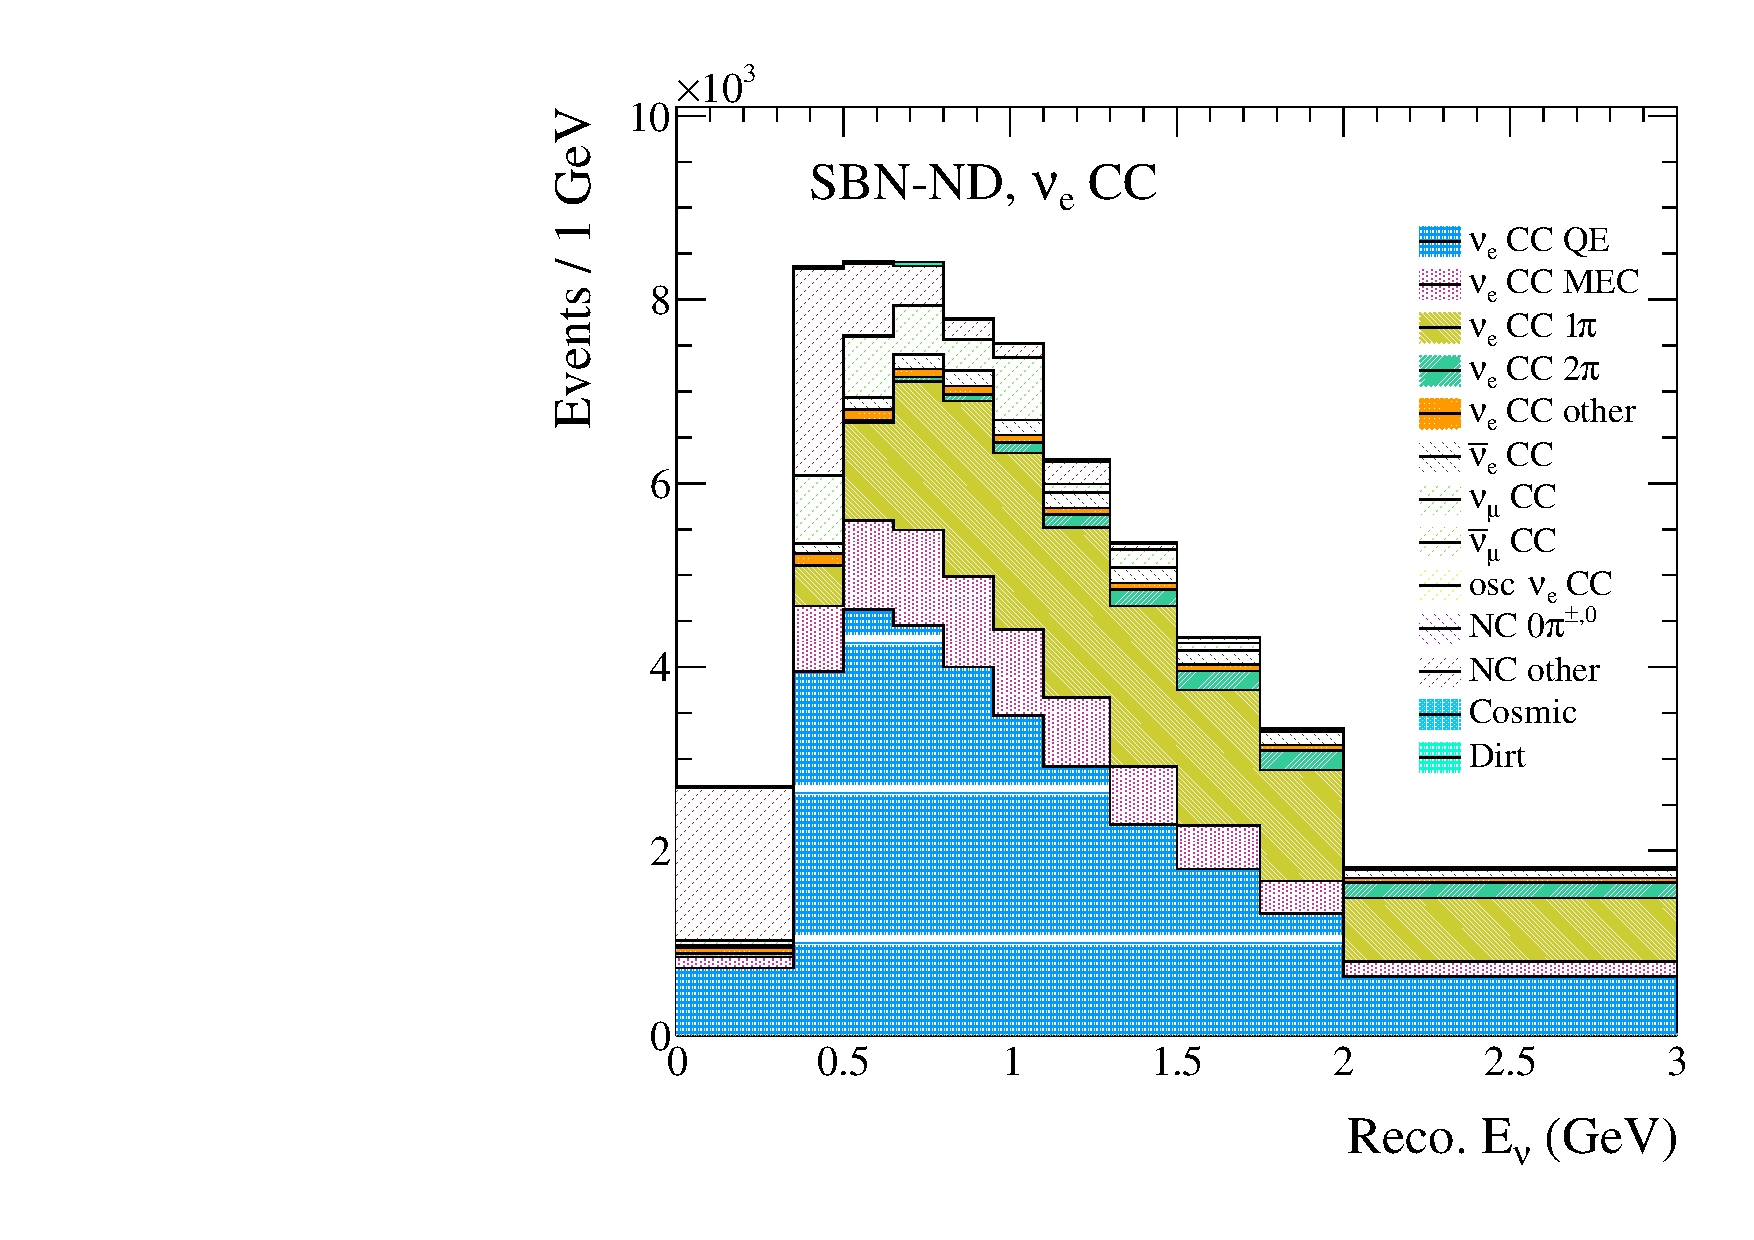
\includegraphics[width=0.49\textwidth]{figures-chap6/spectra/nue_nominal_spectrum_sbn_nd_BNB_FHC_0_modes.pdf}}
  {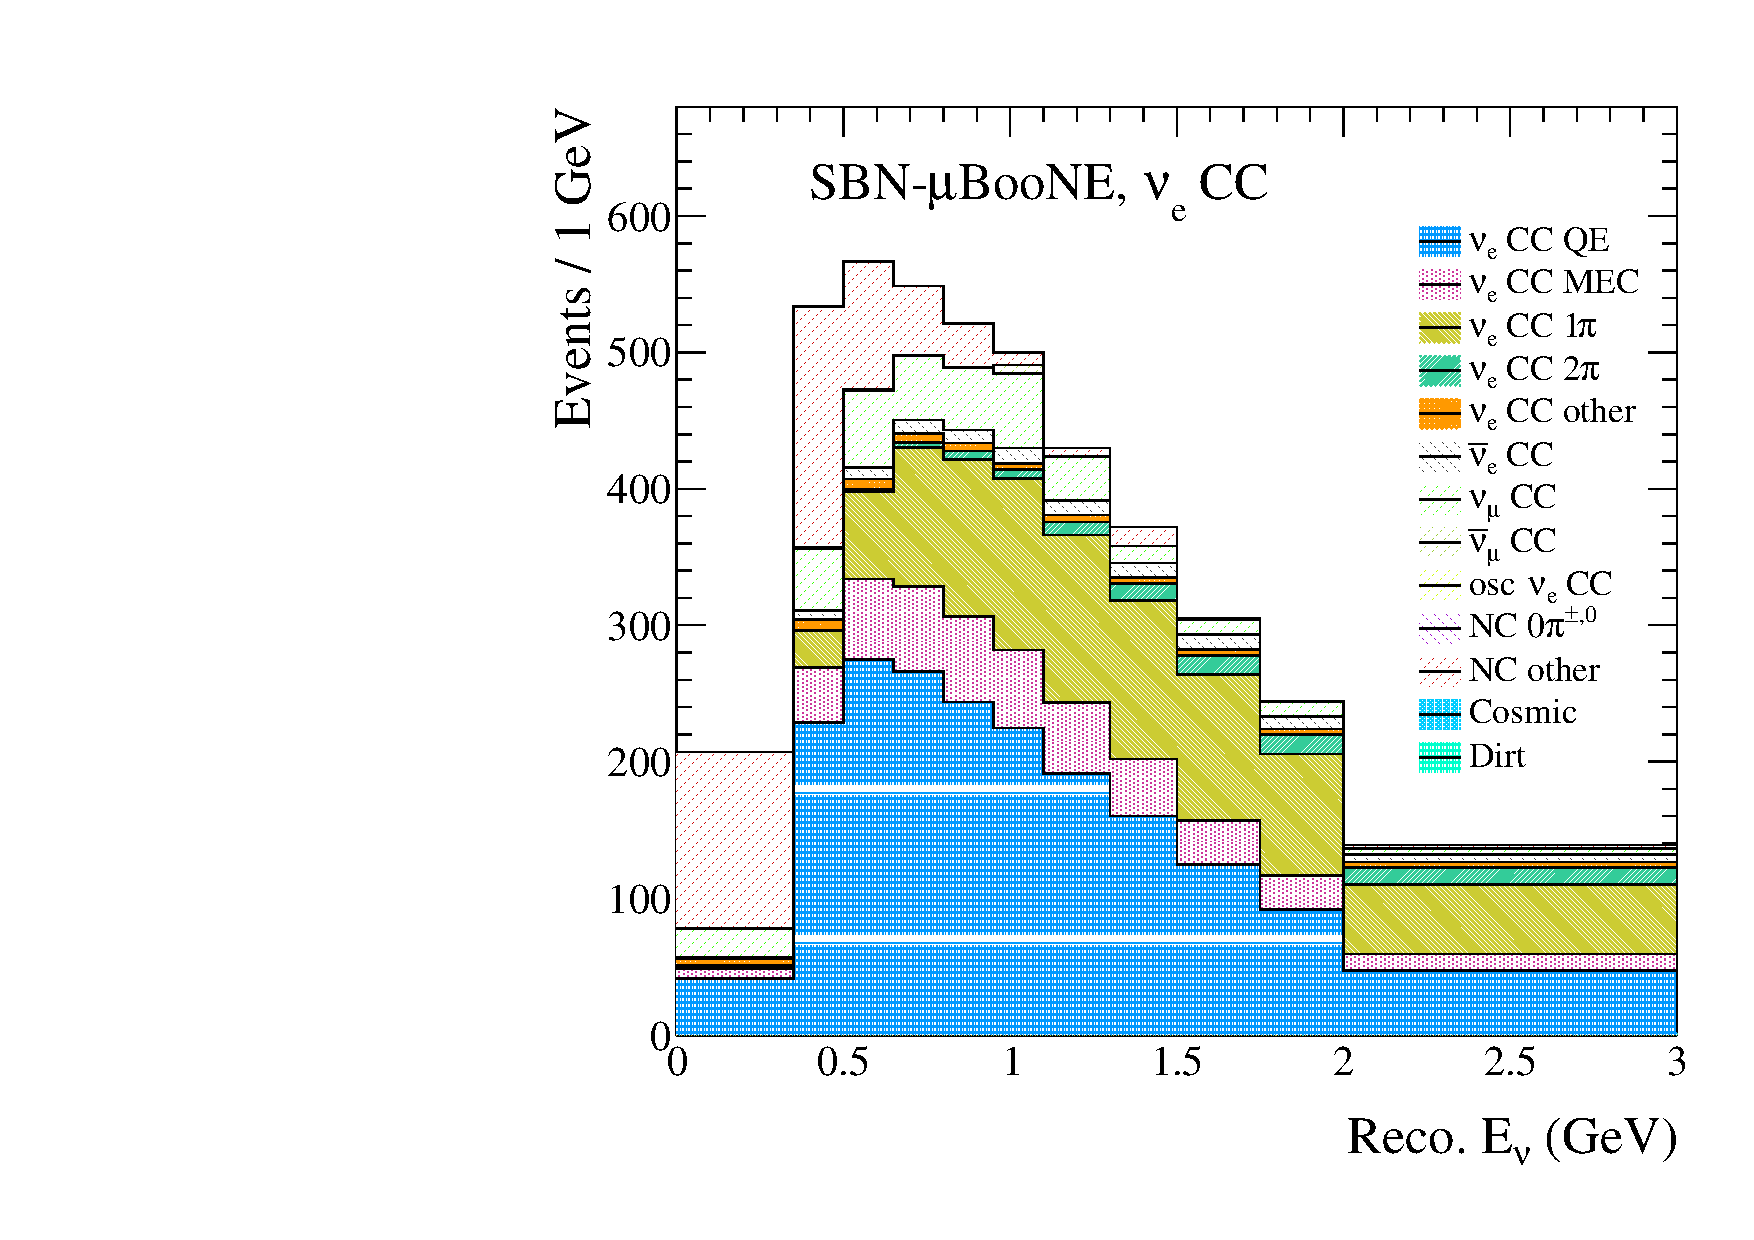
\includegraphics[width=0.49\textwidth]{figures-chap6/spectra/nue_nominal_spectrum_sbn_uboone_BNB_FHC_1_modes.pdf}}
  {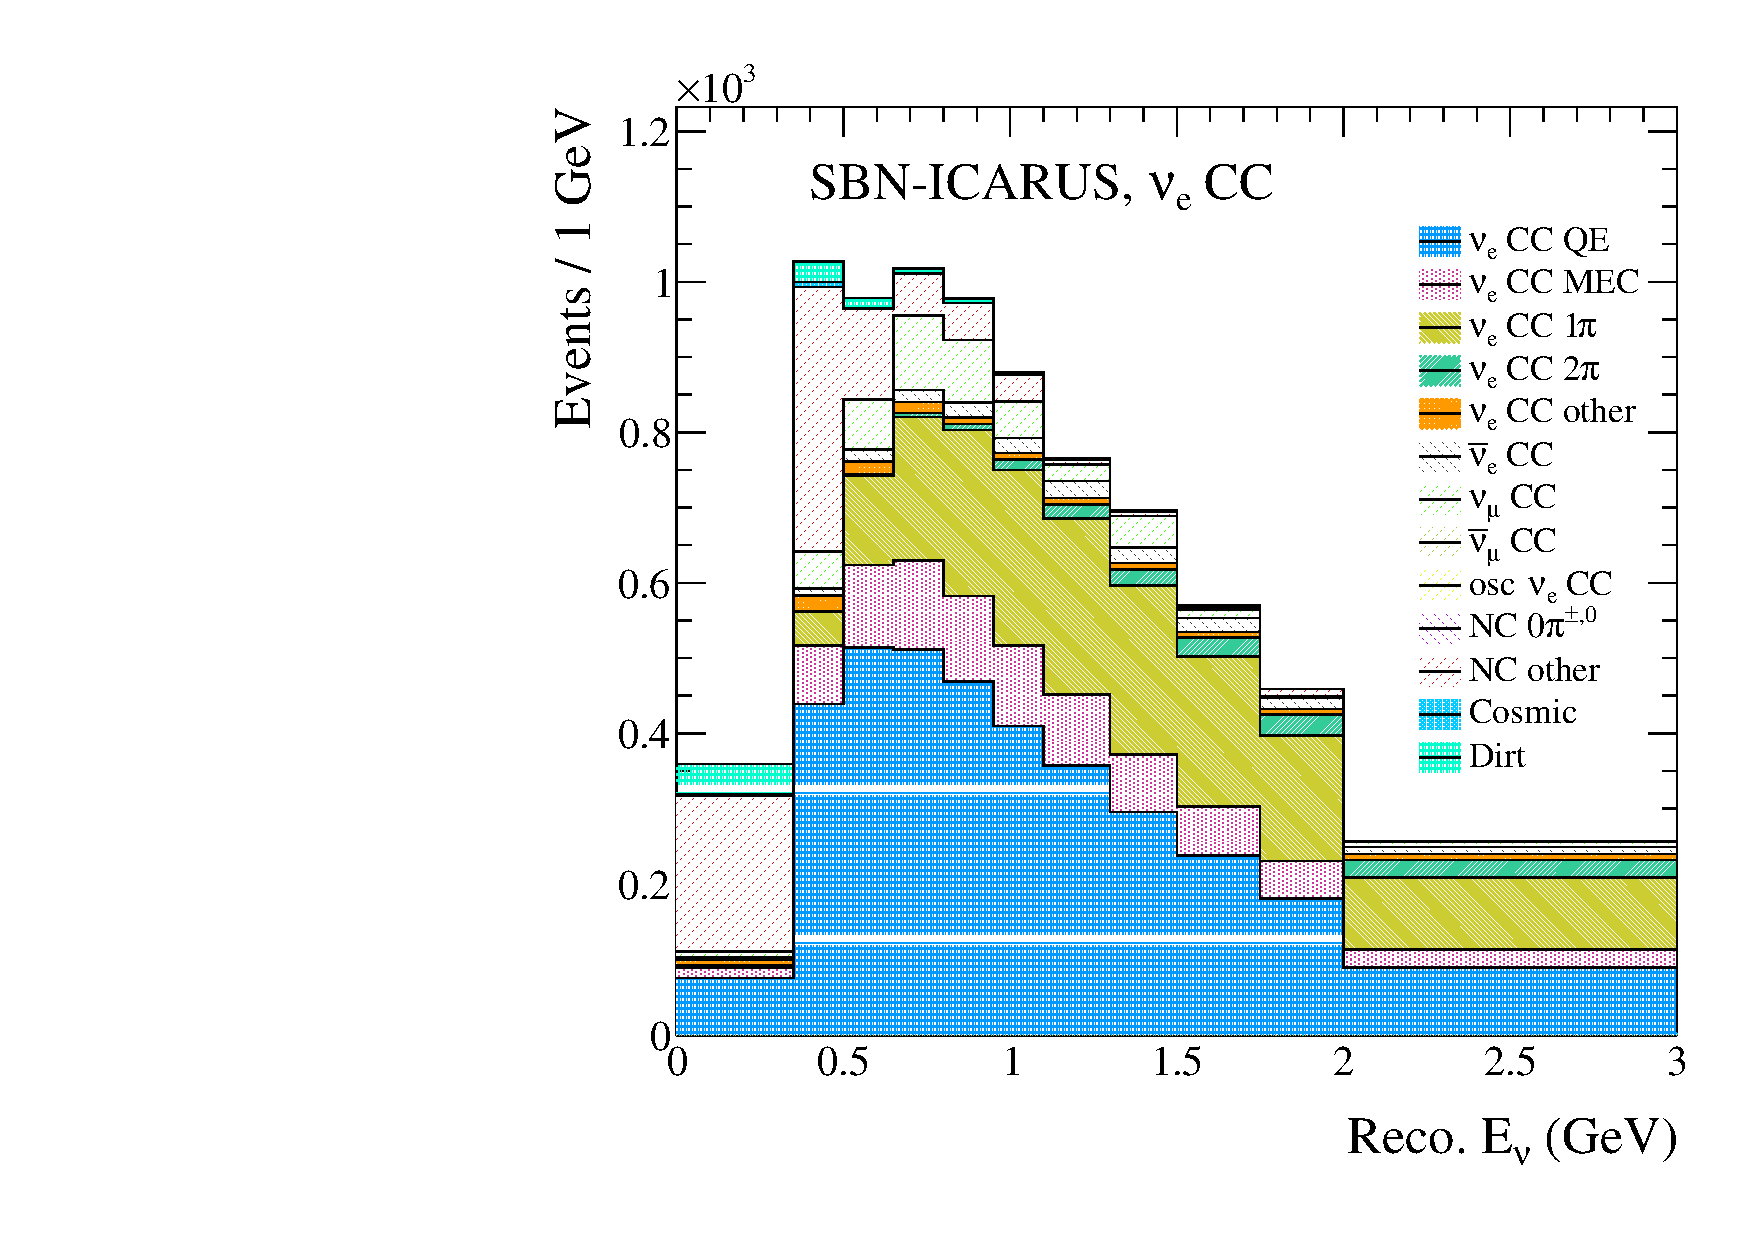
\includegraphics[width=0.49\textwidth]{figures-chap6/spectra/nue_nominal_spectrum_sbn_icarus_BNB_FHC_2_modes.pdf}}
  \captionsetup{width=0.49\textwidth}
  \parbox[b]{0.49\textwidth}%
  {
    \caption[SBN \nue CC inclusive reconstructed neutrino energy spectra.]{SBND (top-left), MicroBooNE (top-right) and ICARUS (bottom)
    reconstructed neutrino energy spectra constructed from the samples of $\nue$~CC~inclusive events. The spectra are broken down into the
    contributions from each neutrino interaction mode.\\ \phantom{.}\\}
    \label{fig:nominal_nue_spectra} 
  }
\end{figure}

\begin{figure}[h!]
  {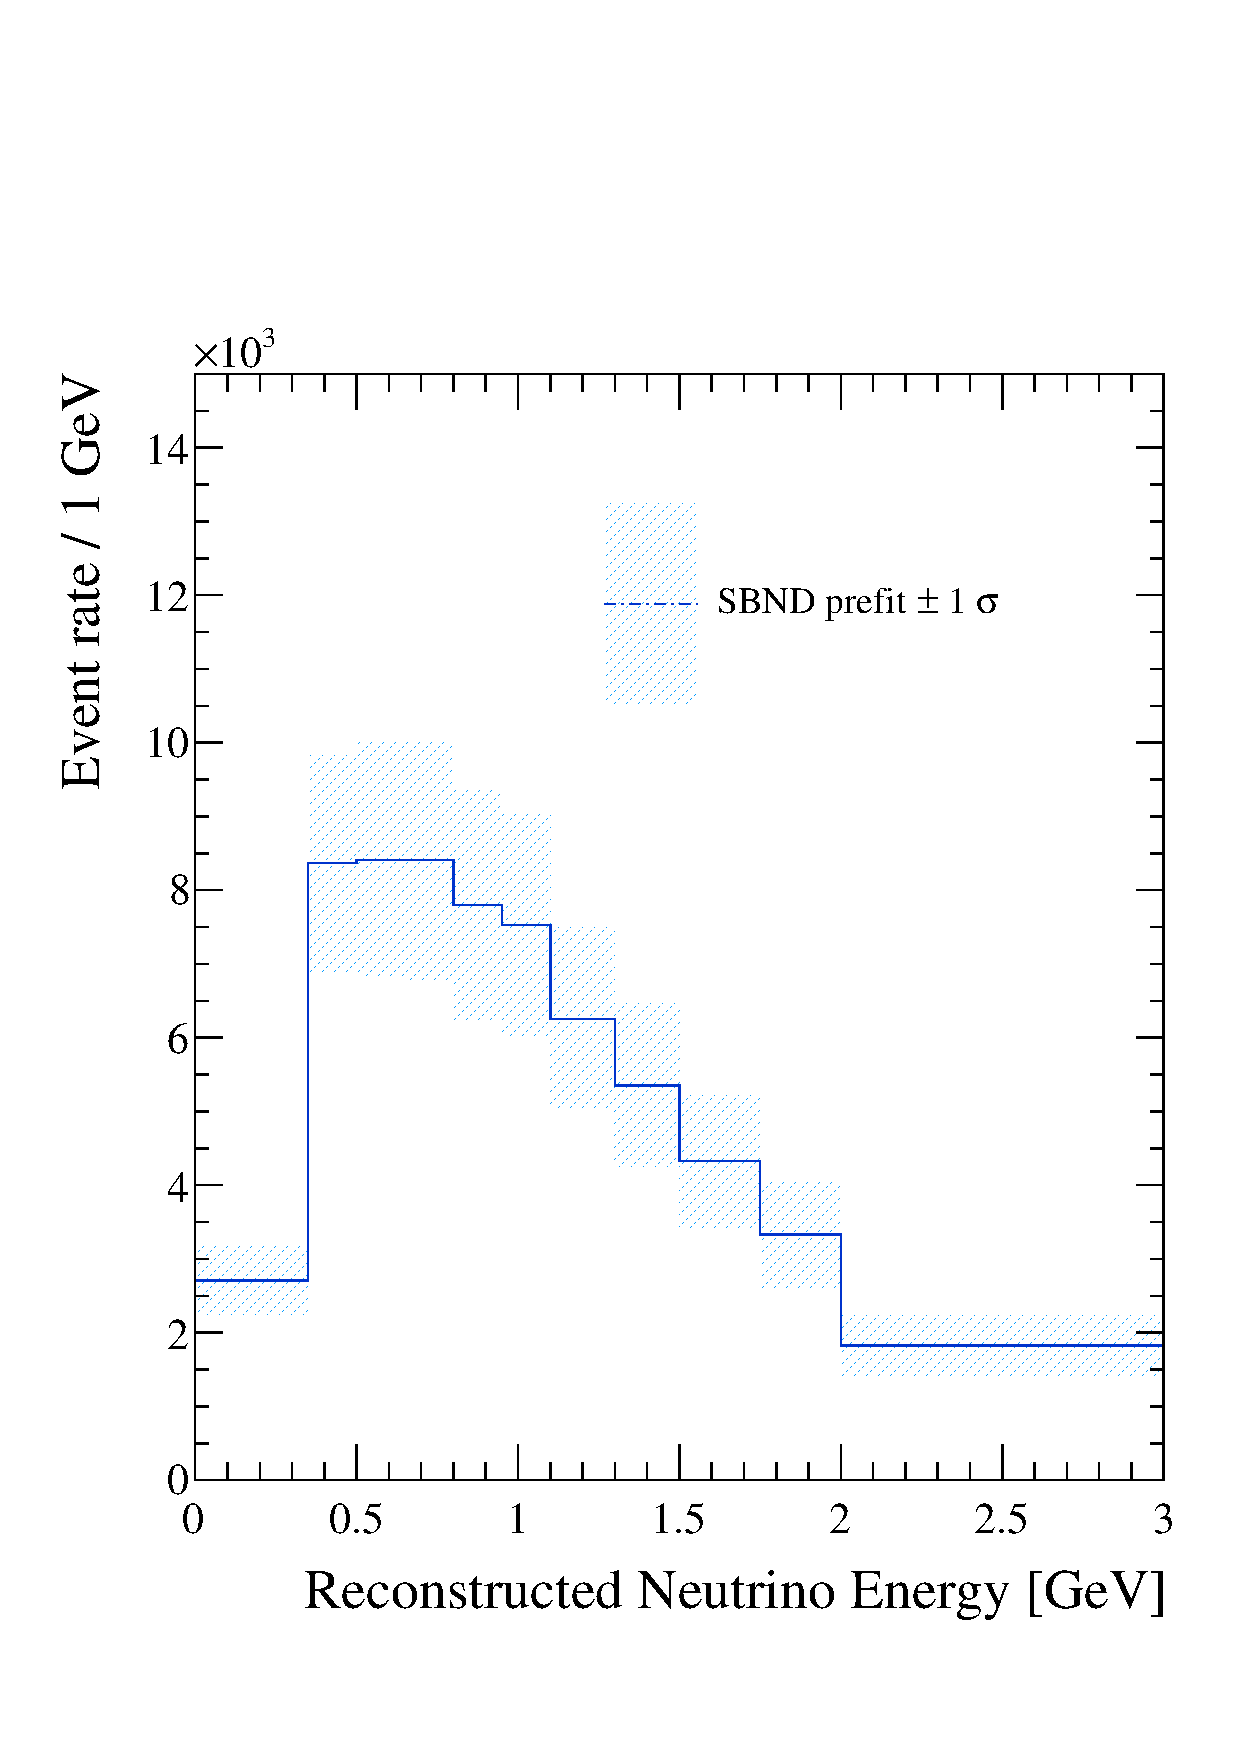
\includegraphics[width=0.49\textwidth]{figures-chap6/spectra/envelopes/sbnd_1sigma_prefit.pdf}}
  {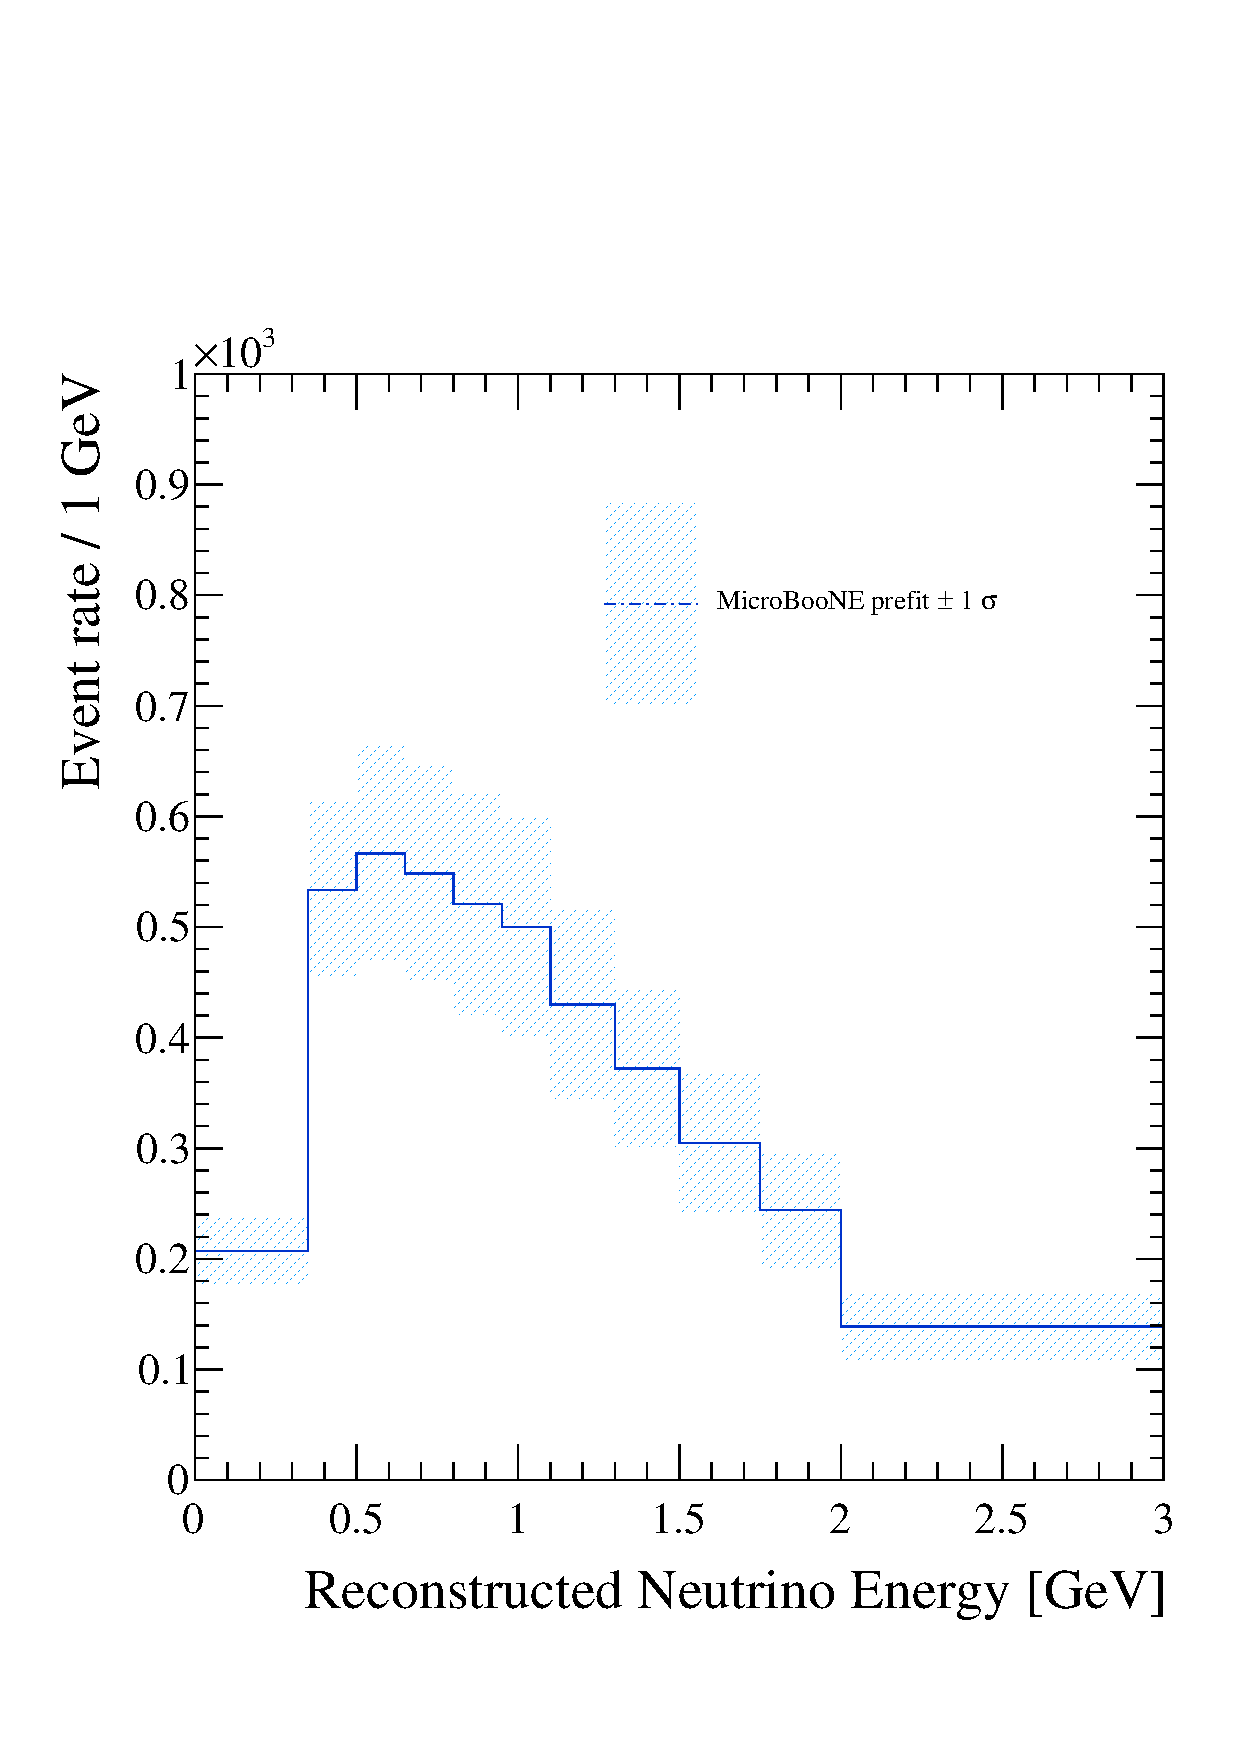
\includegraphics[width=0.49\textwidth]{figures-chap6/spectra/envelopes/uboone_1sigma_prefit.pdf}}
  {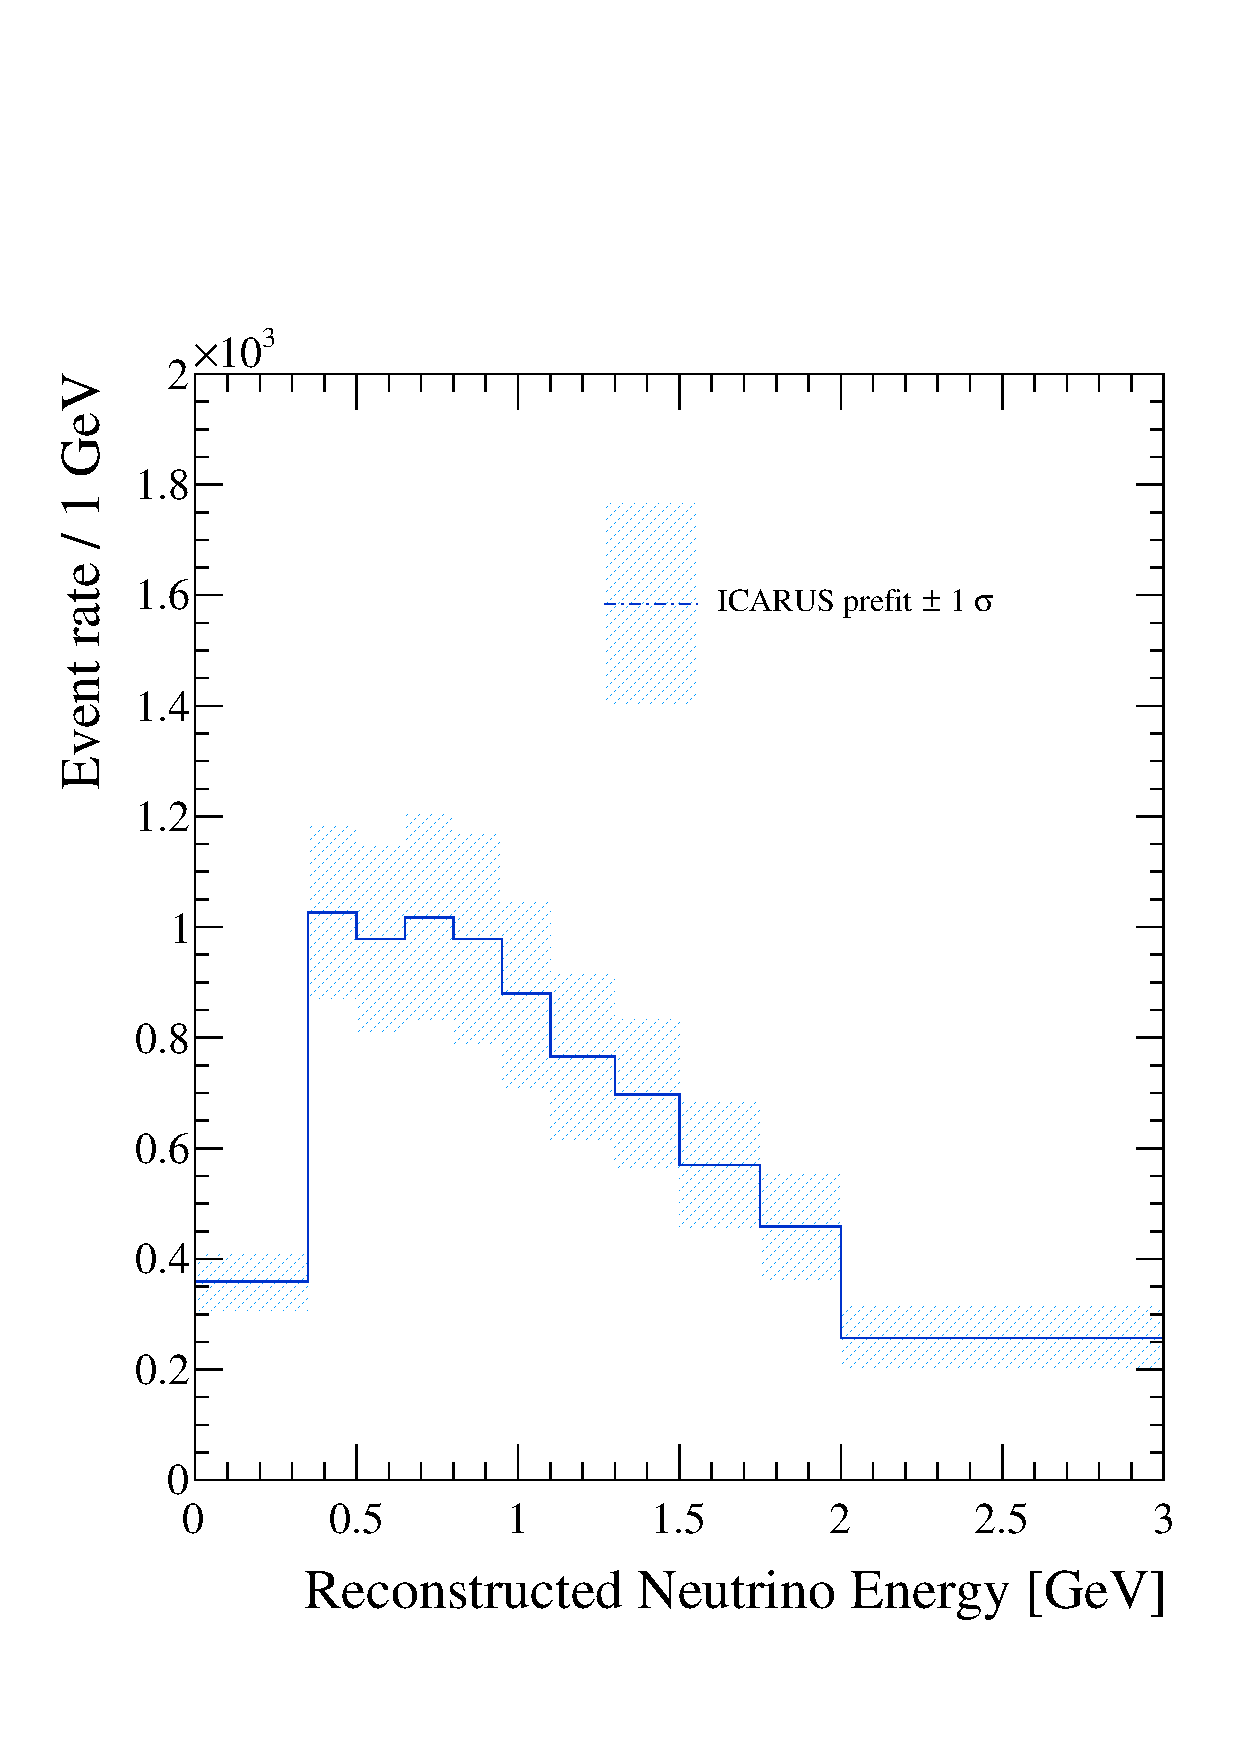
\includegraphics[width=0.49\textwidth]{figures-chap6/spectra/envelopes/icarus_1sigma_prefit.pdf}}
  \captionsetup{width=0.49\textwidth}
  \parbox[b]{0.49\textwidth}%
  {
    \caption[SBN \nue CC inclusive reconstructed neutrino energy spectra with a 1$\sigma$ prefit envelopes.]{SBND (top-left), MicroBooNE (top-right) and ICARUS (bottom) integrated reconstructed neutrino energy spectra constructed from the samples of $\nue$~CC~inclusive events. A 1$\sigma$ prefit uncertainty envelope from the flux and interaction systematics is also shown. \\\phantom{.}\\\phantom{.}\\\phantom{.}\\}
    \label{fig:nominal_nue_spectra_1sigma_enevelope} 
  }
\end{figure}

\begin{figure}[h!]
    \centering
    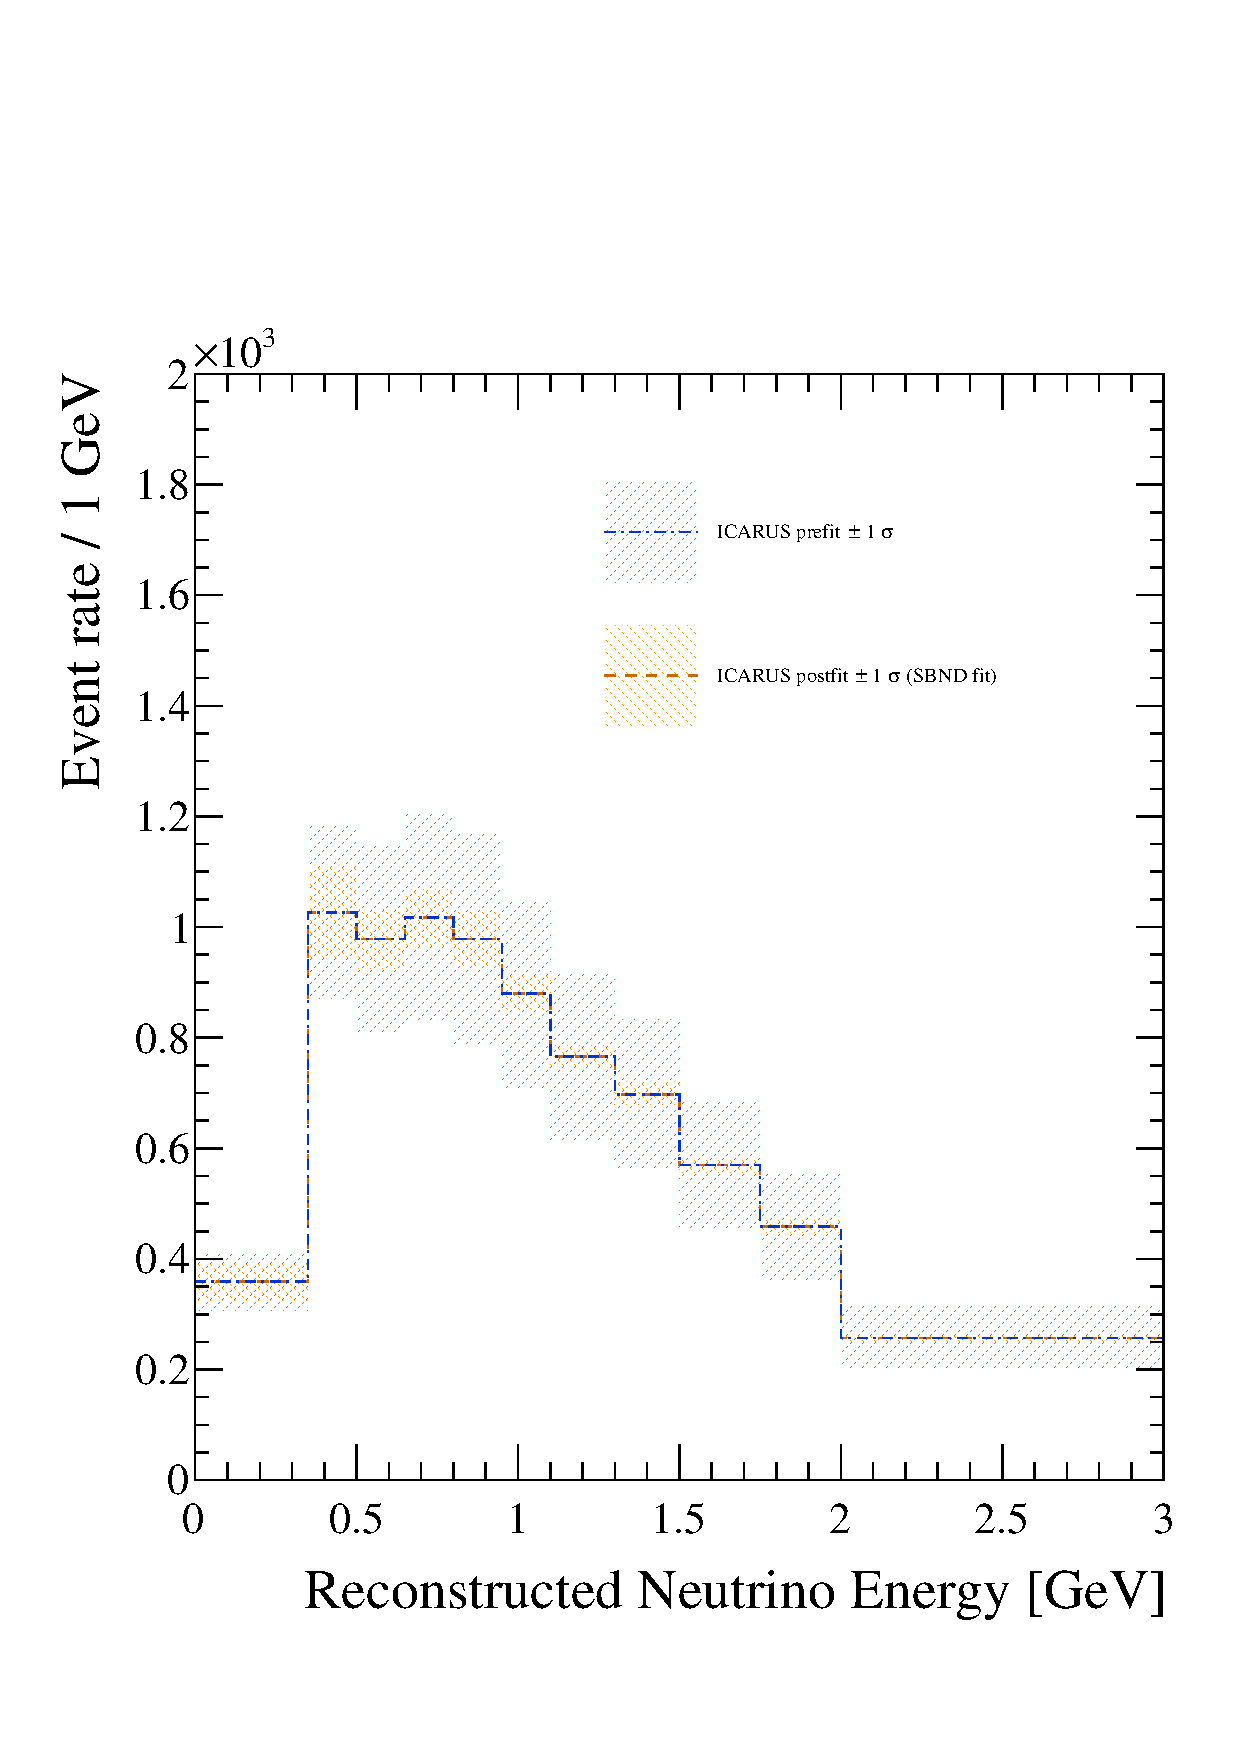
\includegraphics[width = \largefigwidth]{figures-chap6/spectra/envelopes/icarus_pre_post_fit_nue.pdf}
    \caption[ICARUS \nue CC inclusive neutrino energy spectra with a 1$\sigma$ prefit and postfit envelope.]{ICARUS integrated reconstructed neutrino energy spectrum constructed from the samples of \nue~CC~inclusive events. The $1\sigma$ prefit envelope is shown as well as a $1\sigma$ postfit envelope based on a SBND fit. The reduction in size of the error envelope when going from prefit to postfit shows the impact of SBND on improving the accuracy of the ICARUS prediction.}
    \label{fig:icarus_pre_post_fit}
\end{figure}

\clearpage
\subsection{\texorpdfstring{\nue Appearance Analysis}{nue Appearance Analysis}}\label{sec:nue_app}

The \nue appearance channel is concerned with oscillations from \numu to \nue and since the oscillation channels are currently considered as stand-alone analyses, an increase in the event rate is expected. This is shown in \FigureRef{fig:nue_spectra_with_osc_overlay} where the nominal event rate breakdown is shown as in \FigureRef{fig:nominal_nue_spectra}, but overlayed with and integrated spectrum that was produced with oscillation parameters $\sin^2{2\theta_{\mu e}} = 0.003$ and $\Delta m^2_{41} = 1.32 \text{ eV}^2$. The oscillation signal seen for these parameters in \gls{sbnd} is small whereas for \gls{microboone} and \gls{icarus} it is substantial which is consistent with what is seen in \FigureRef{fig:osc_probability}. This highlights the fact that \gls{sbnd} will largely be used to constrain parameters due to observing no or very few oscillated events with the oscillation signal being largely left to \gls{microboone} and \gls{icarus}. 


\begin{figure}[h!]
  {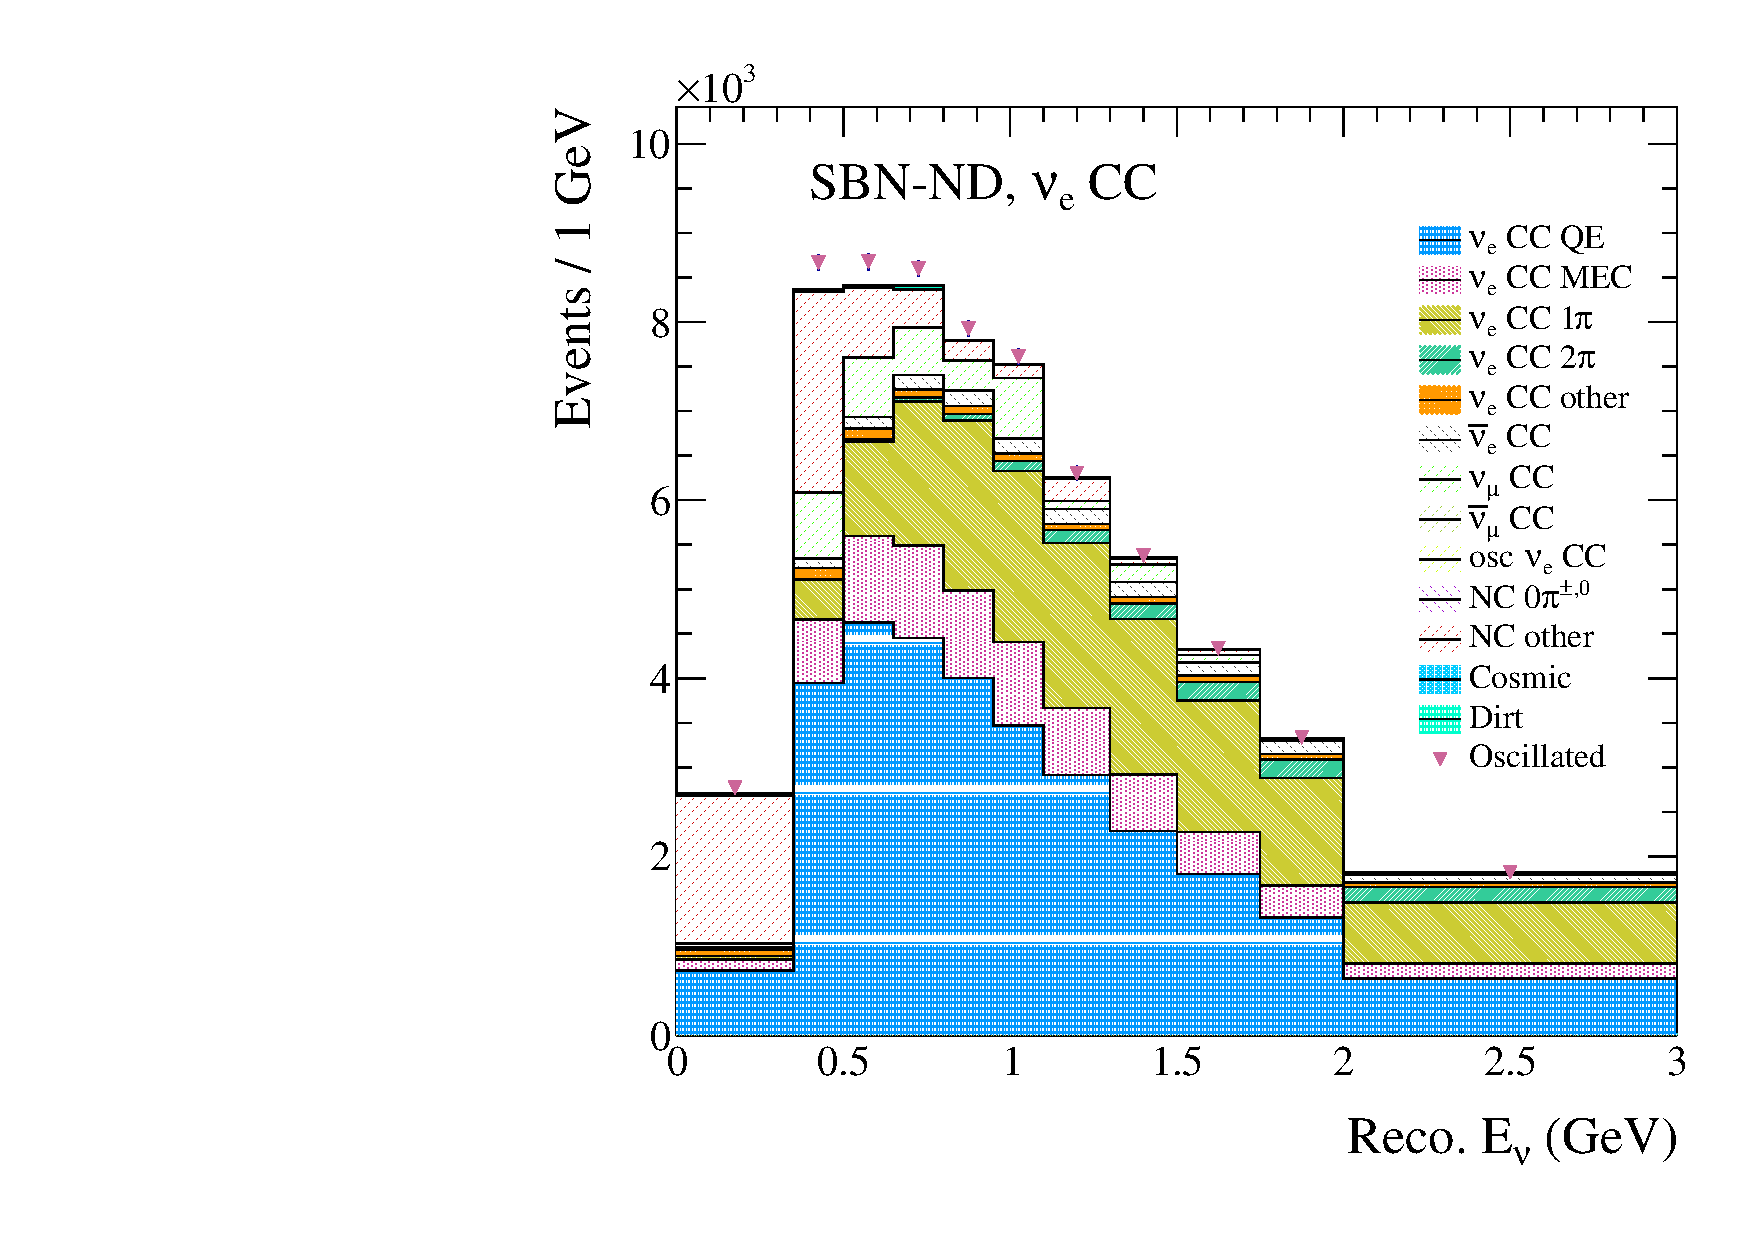
\includegraphics[width=0.49\textwidth]{figures-chap6/spectra/nue_app_dmsq_1.32_sinsq_0.003_overlay_spectrum_sbn_nd_BNB_FHC_0_modes.pdf}}
  {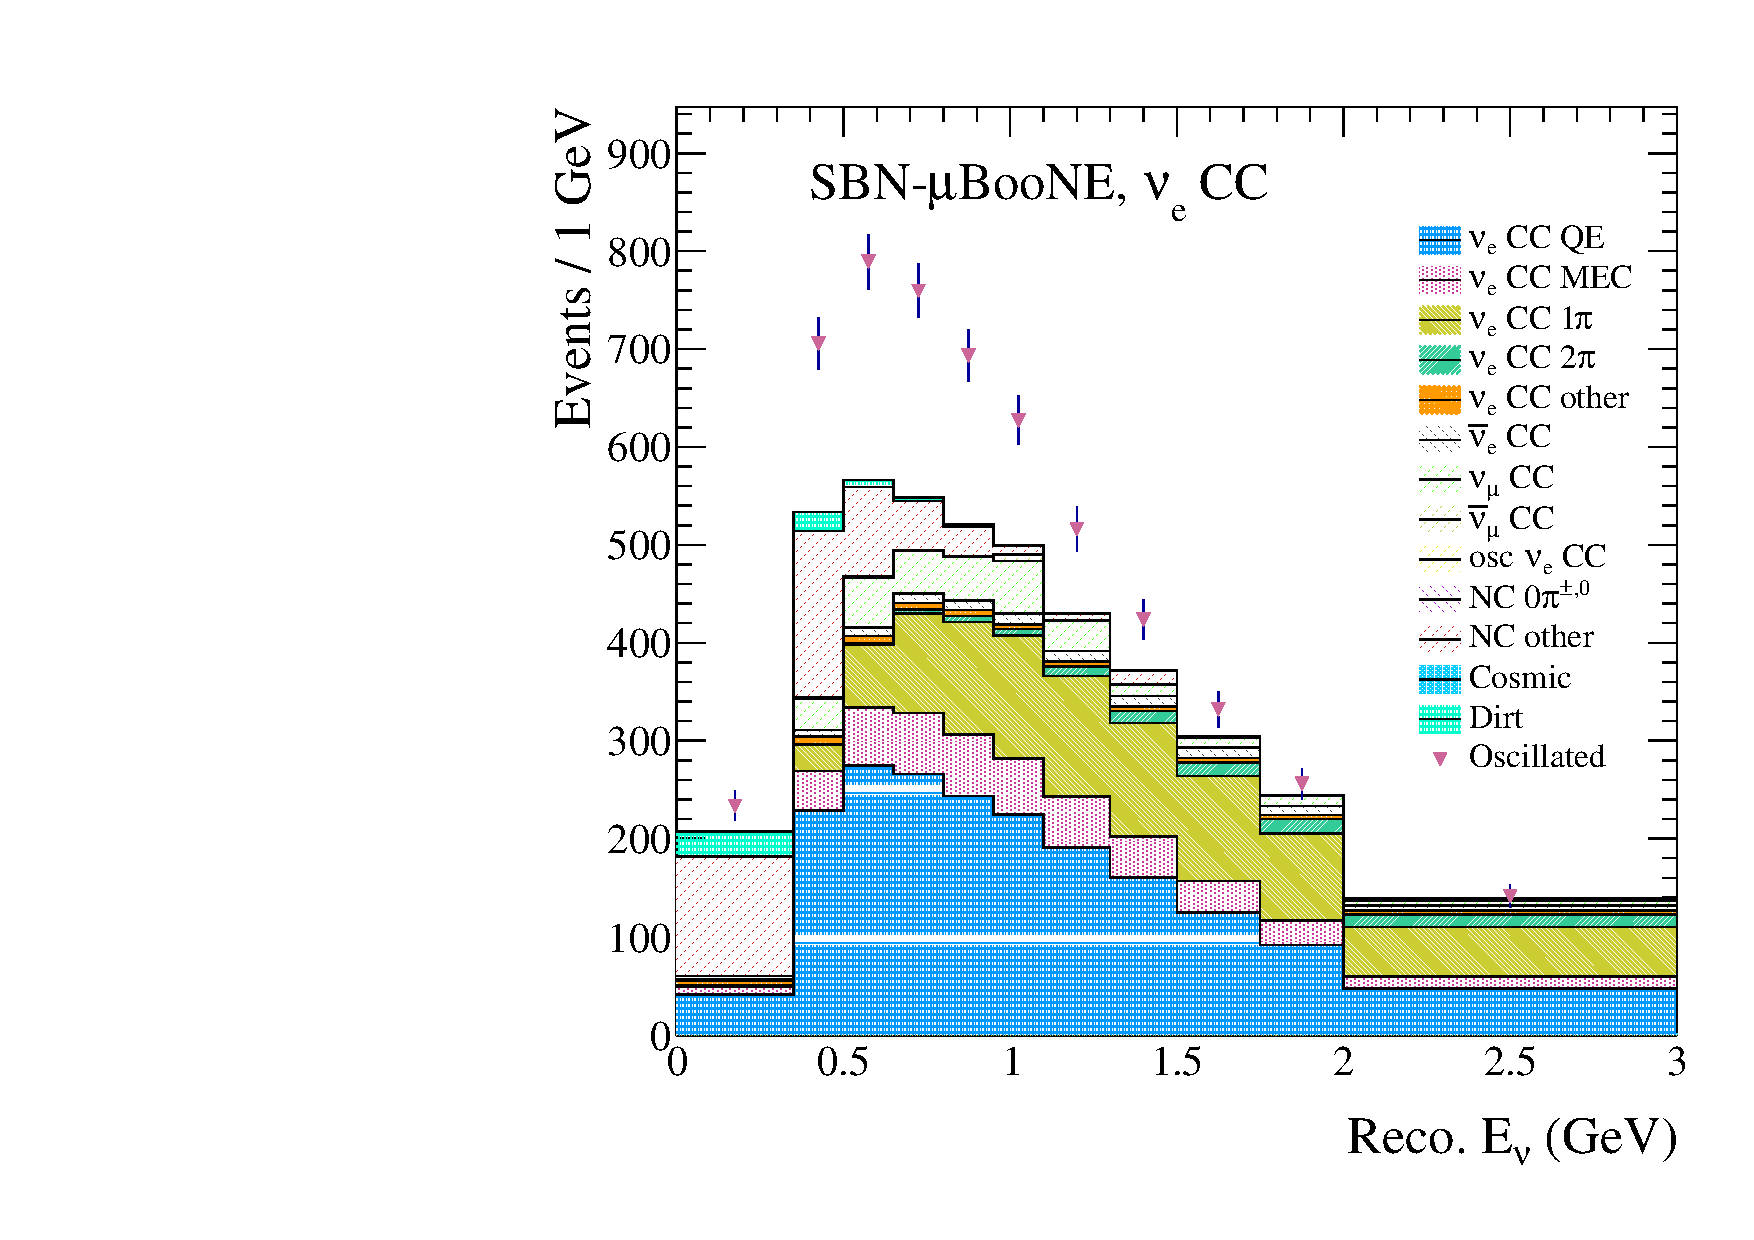
\includegraphics[width=0.49\textwidth]{figures-chap6/spectra/nue_app_dmsq_1.32_sinsq_0.003_overlay_spectrum_sbn_uboone_BNB_FHC_1_modes.pdf}}
  {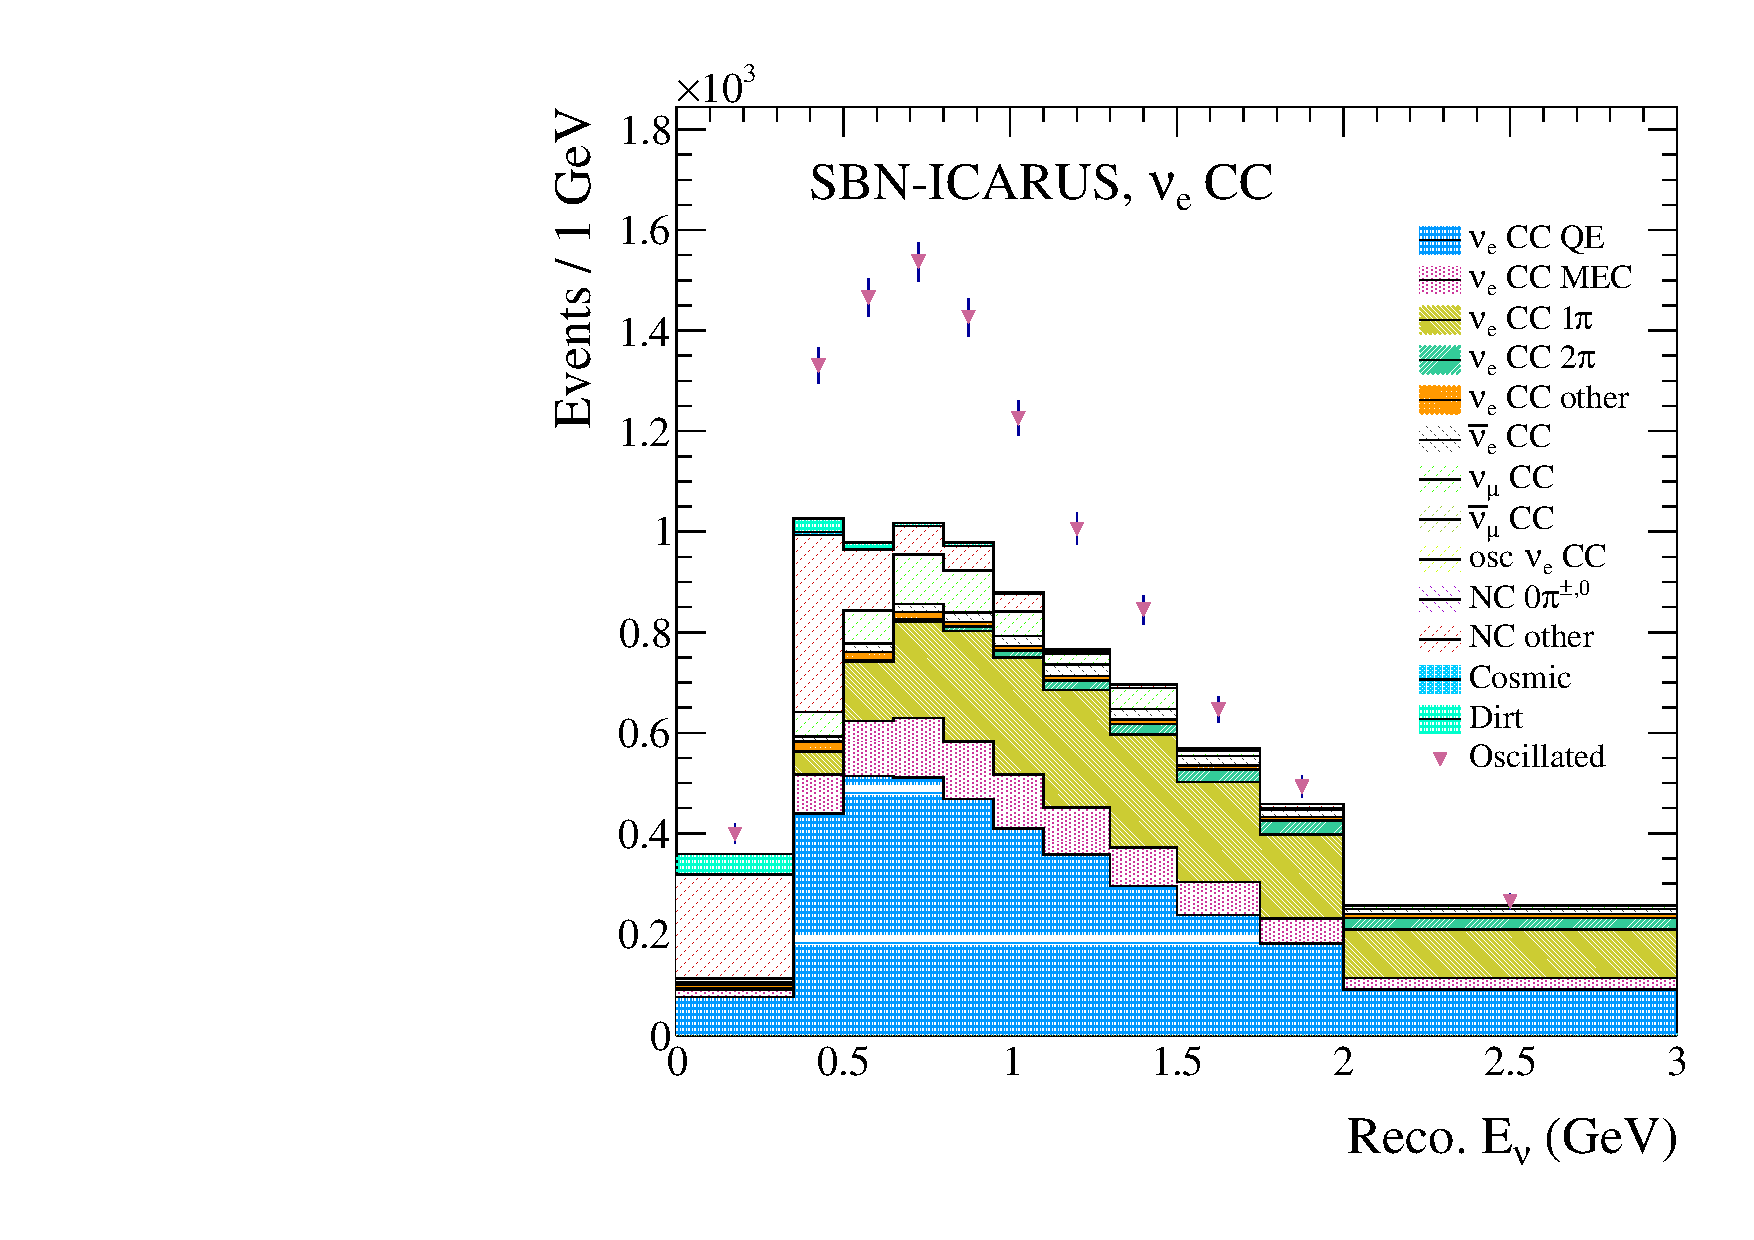
\includegraphics[width=0.49\textwidth]{figures-chap6/spectra/nue_app_dmsq_1.32_sinsq_0.003_overlay_spectrum_sbn_icarus_BNB_FHC_2_modes.pdf}}
  \captionsetup{width=0.49\textwidth}
  \parbox[b]{0.49\textwidth}%
  {
    \caption[SBN \nue appearance CC inclusive reconstructed neutrino energy spectra with oscillated spectrum overlayed.]{The nominal spectra as in \FigureRef{fig:nominal_nue_spectra} but an additional integrated oscillated spectrum with oscillation parameters, $\sin^2{2\theta_{\mu e}} = 0.003$ and $\Delta m^2_{41} = 1.32$ eV$^2$ has been overlayed showing the increase in event rate. \\\phantom{.}\\\phantom{.}\\\phantom{.}\\
    \label{fig:nue_spectra_with_osc_overlay}}
    }
\end{figure}

\newpage
The top left plot of Figure~\ref{fig:Nue_app_spectra_ratios} shows the \nue appearance stat only exclusion contour and allowed region from fits combining all three \gls{sbn} detectors. The injected point $\Delta m^2_{41} = 1.32$ eV$^2$, $\sin^2{2\theta_{\mu e}} = 0.003$, used when producing the allowed region is shown along with two further points on the exclusion contour at $\Delta m^2_{41} = 1$ eV$^2$, $\sin^2{2\theta_{\mu e}} = 0.0014$ and $\Delta m^2_{41} = 100$ eV$^2$, $\sin^2{2\theta_{\mu e}} = 0.0005$. \nue appearance spectra are produced using oscillation parameters corresponding to each of these three points for each of the three SBN detectors. The ratio of each of these oscillated spectra to the nominal for each detector are shown in the the remaining plots in Figure~\ref{fig:Nue_app_spectra_ratios} and highlight the expected oscillation signal.


\begin{figure}[h!]
    \centering
    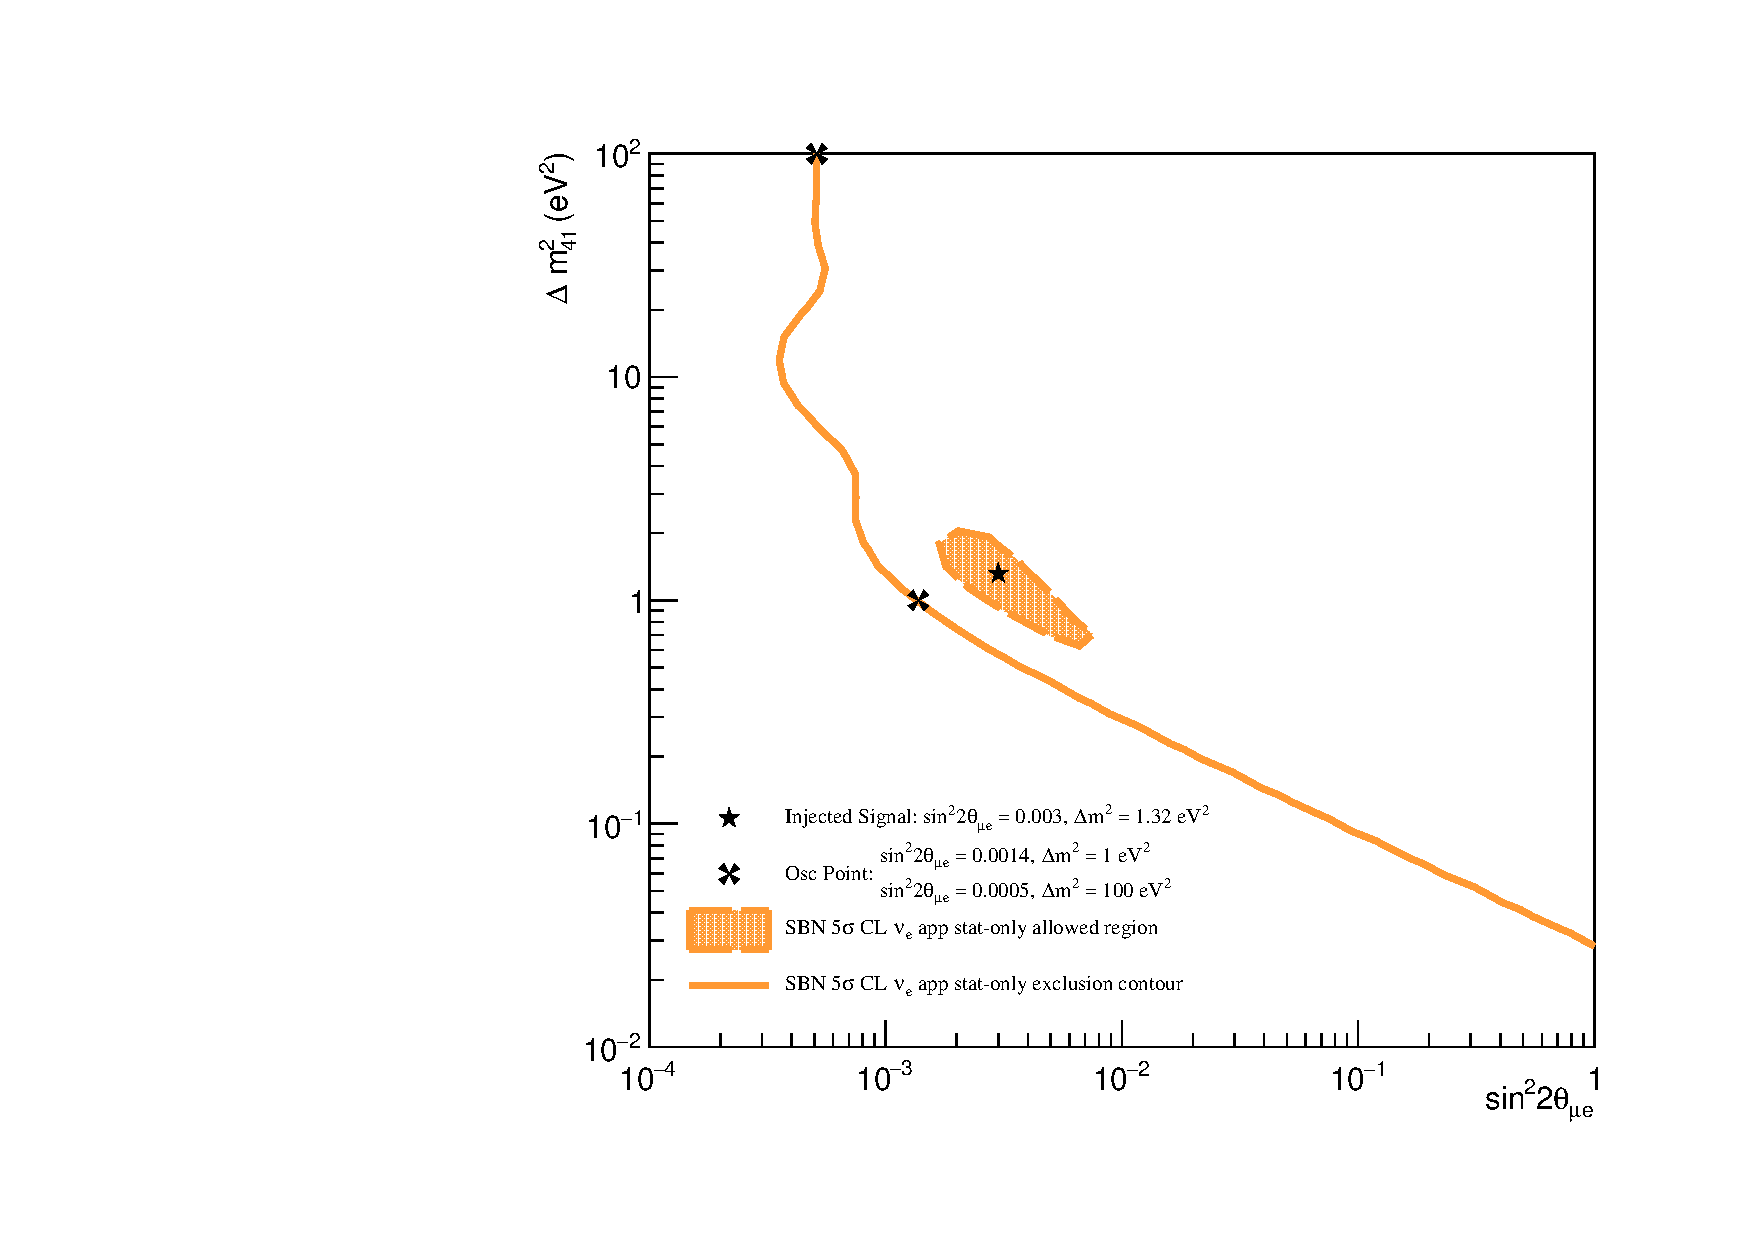
\includegraphics[width = 0.49\textwidth, height = 0.47\textwidth]{figures-chap6/overlays/nue_app_stat_osc_markers.pdf}
    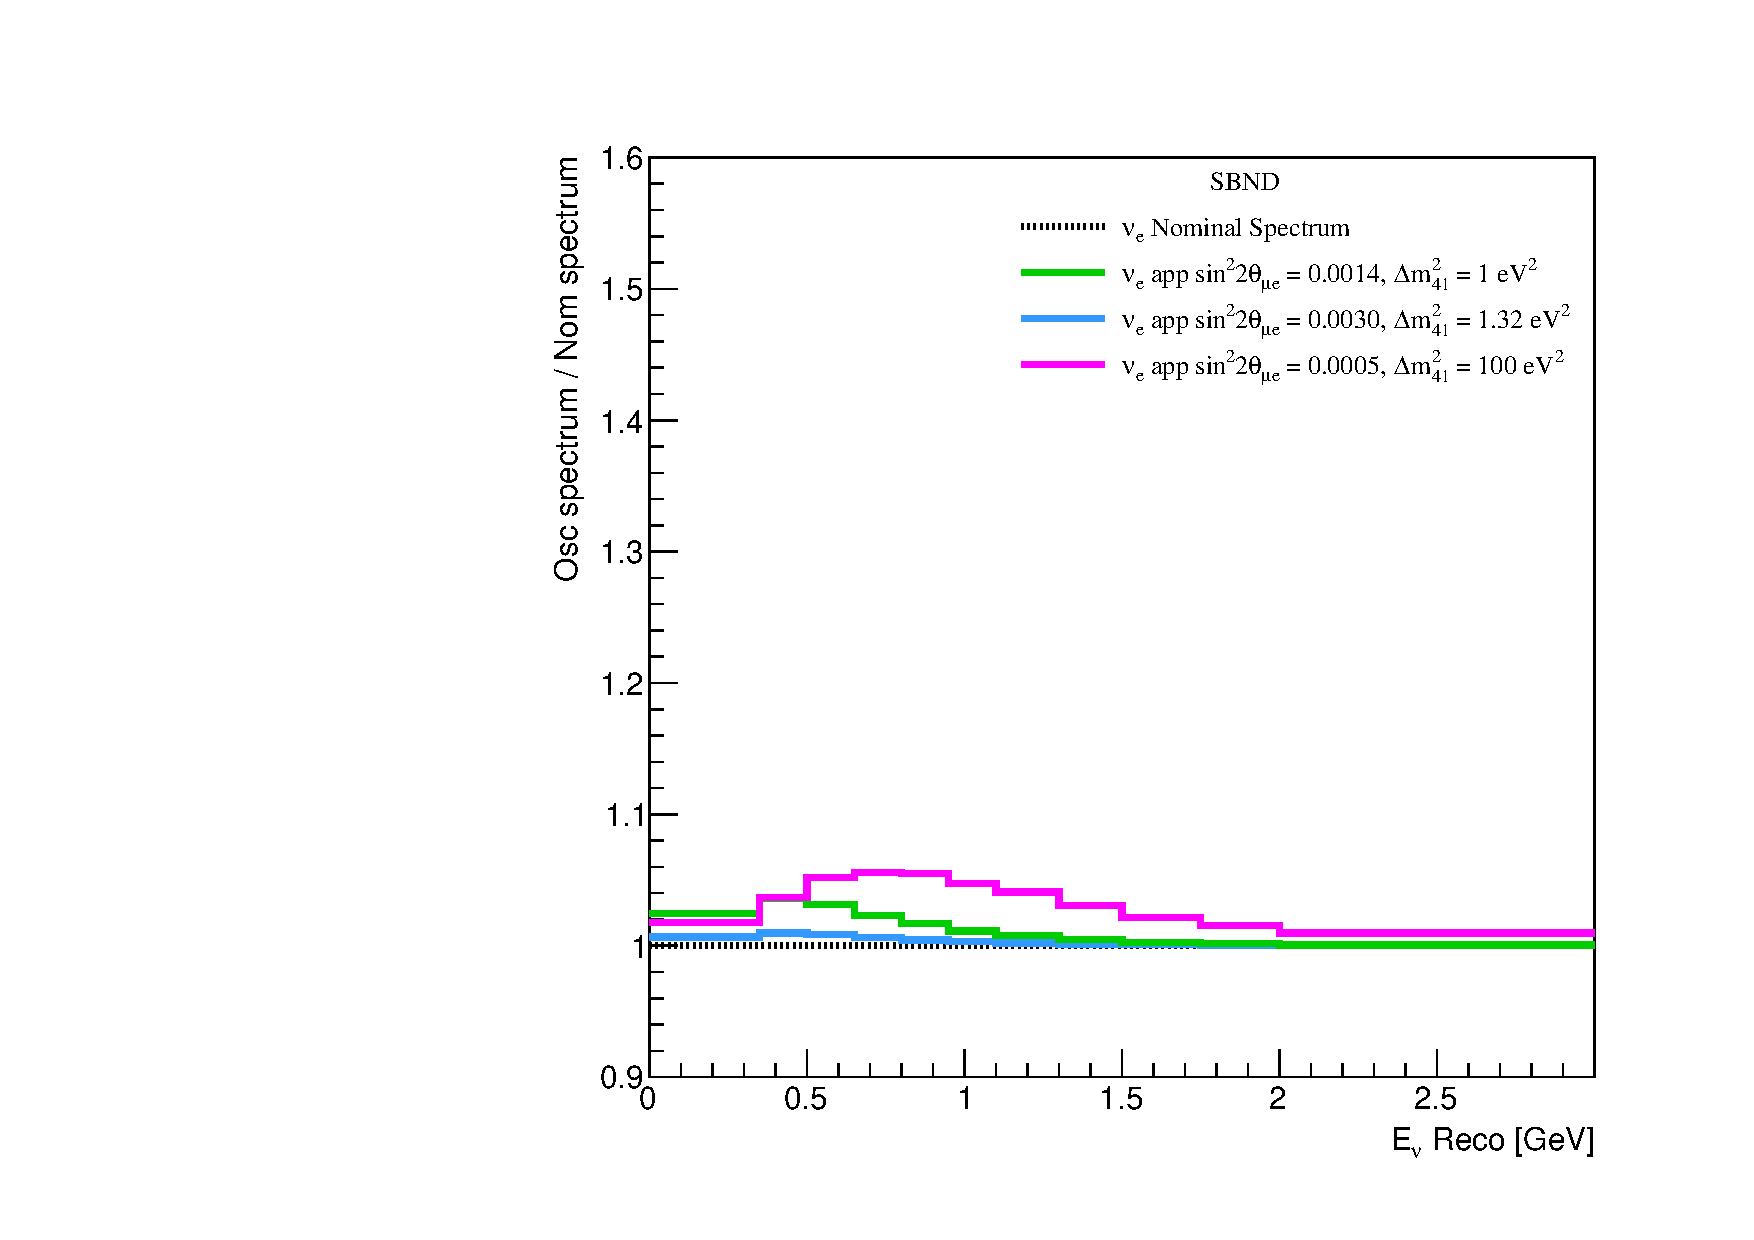
\includegraphics[width = 0.49\textwidth]{figures-chap6/spectra/nue_app_spectra_ratio_sbnd.pdf}
    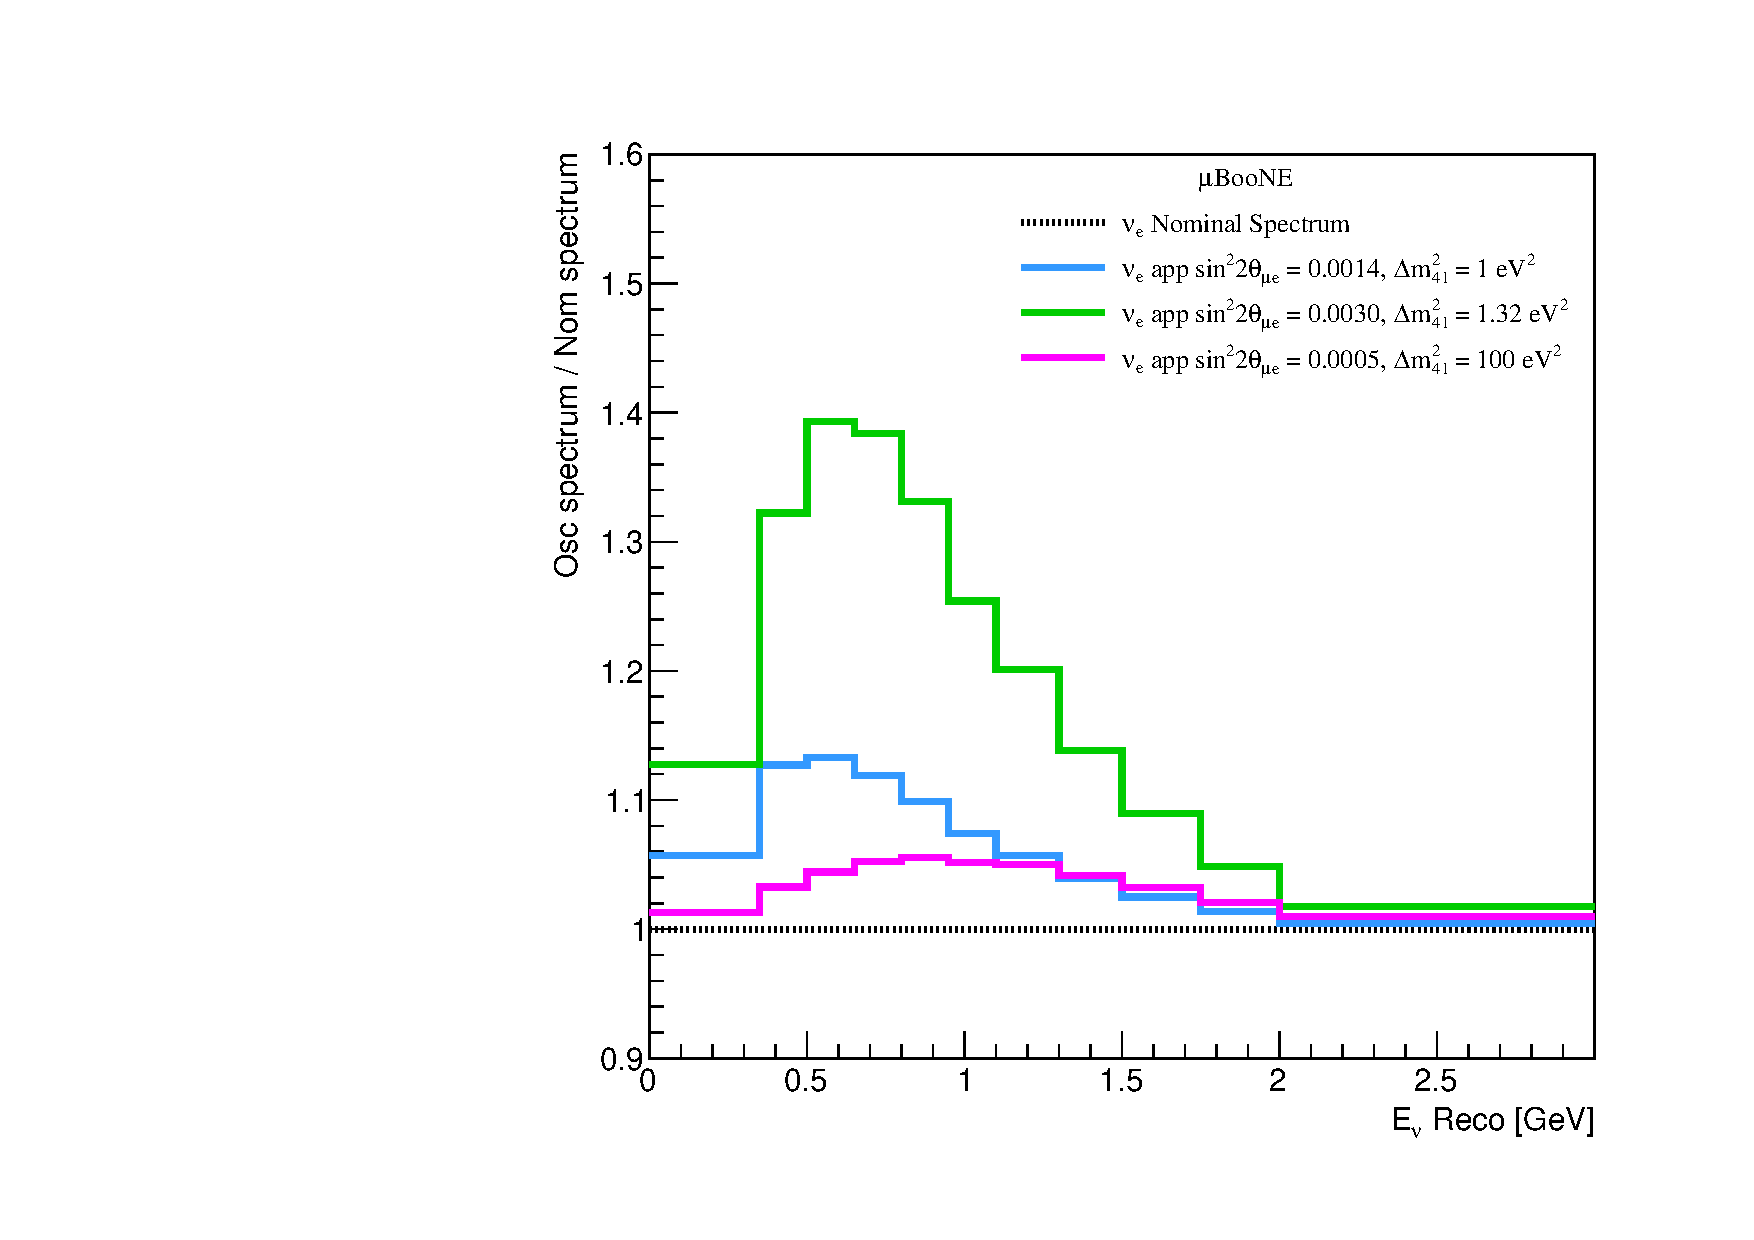
\includegraphics[width = 0.49\textwidth]{figures-chap6/spectra/nue_app_spectra_ratio_uboone.pdf}
    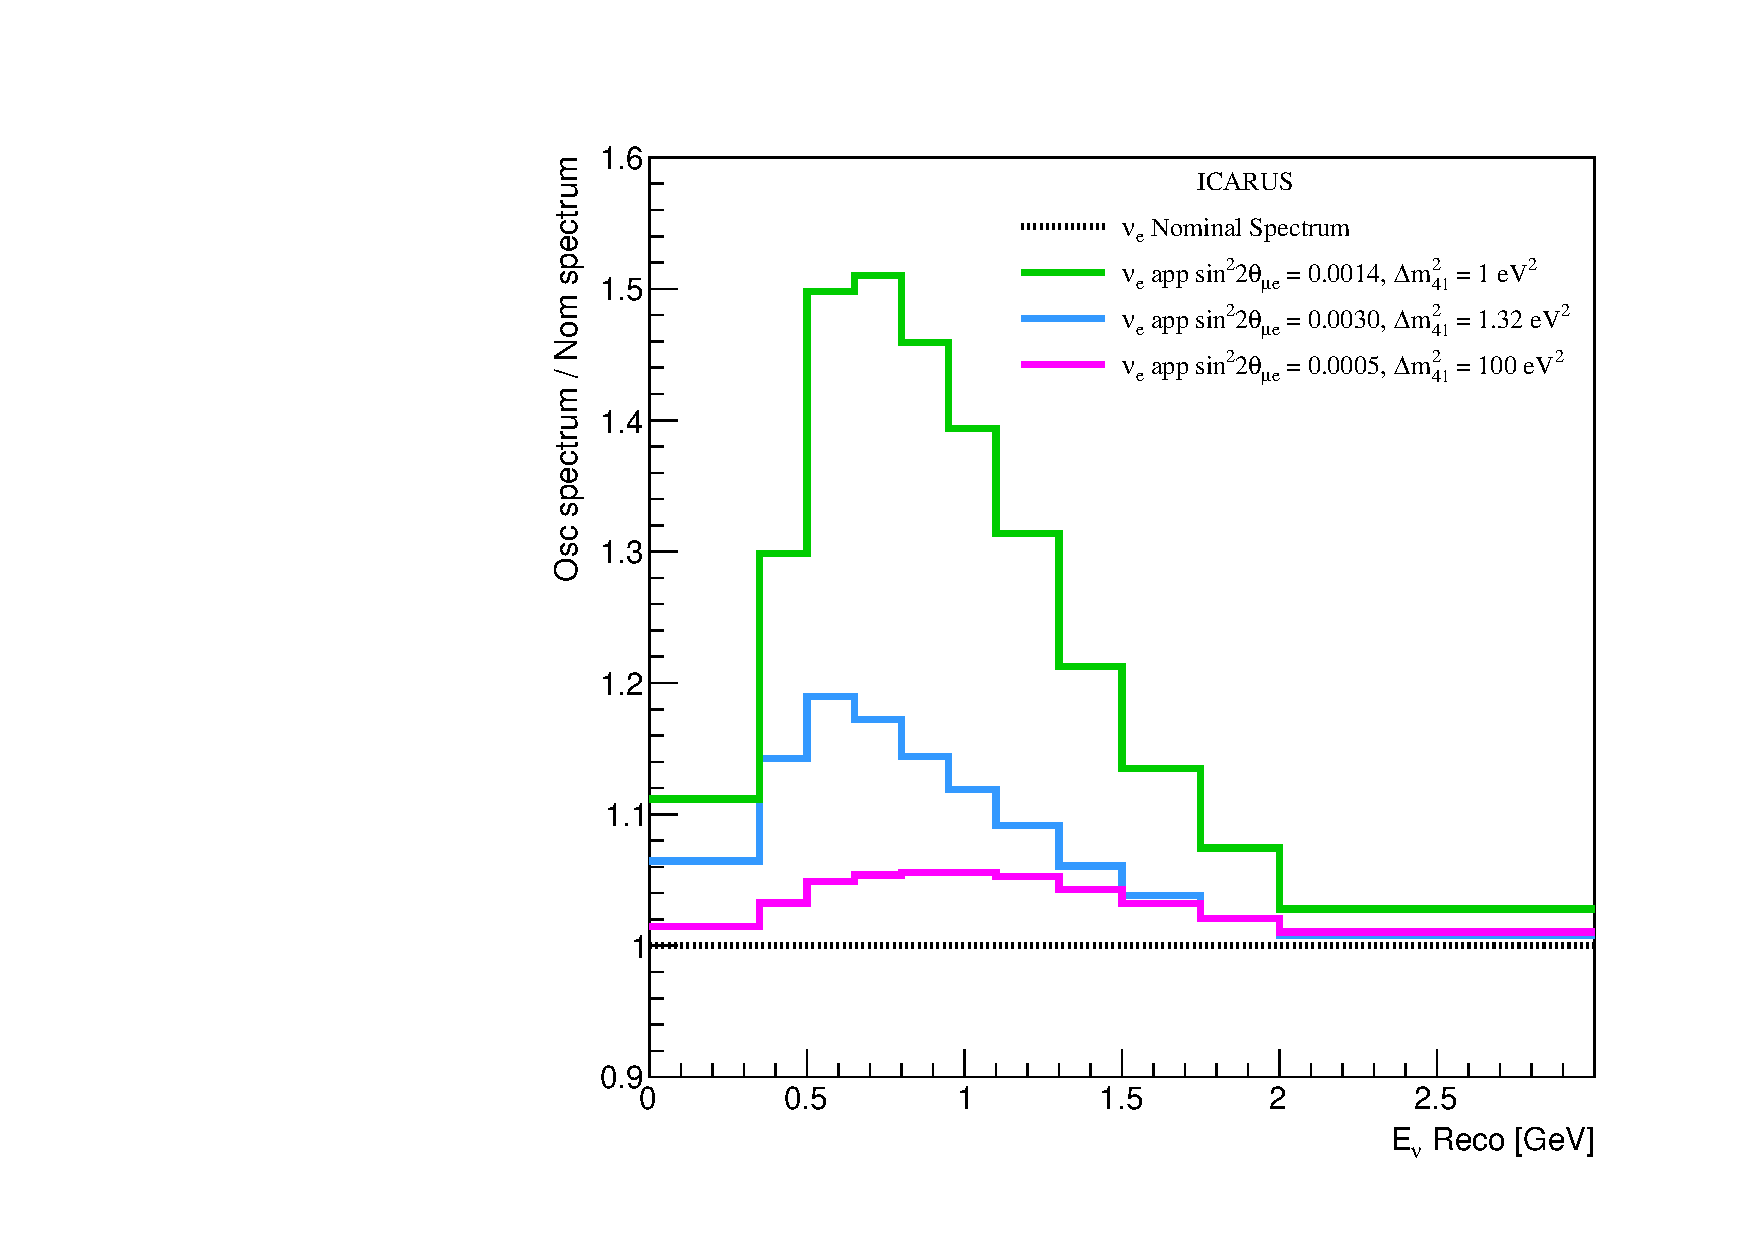
\includegraphics[width = 0.49\textwidth]{figures-chap6/spectra/nue_app_spectra_ratio_icarus.pdf}
    \caption[Ratio of \nue appearance spectra with the oscillation parameters shown on the statistical only contour.]{\nue appearance stat-only exclusion contour and allowed region. The injected point at $\sin^2{2\theta_{\mu e}} = 0.003$, $\Delta m^2_{41}$ = 1.32 eV$^2$ used for the allowed region is shown along with two further points at $\sin^2{2\theta_{\mu e}} = 0.0014$, $\Delta m^2_{41}$ = 1 eV$^2$ and   $\sin^2{2\theta_{\mu e}} = 0.0005$, $\Delta m^2_{41}$ = 100 eV$^2$ (top left). The ratio of spectra with oscillation parameters corresponding to the three points mentioned versus nominal are shown for sbnd (top right), MicroBooNE (bottom left) and ICARUS (bottom right).}
    \label{fig:Nue_app_spectra_ratios}
\end{figure}


An example of the $\chi^2$ surface as described in \SectionRef{sec:VALOR_framework} is shown in \FigureRef{fig:nue_app_chisq_surface} along with contours of constant $\chi^2$ corresponding to 90\%, $3\sigma$ and $5\sigma$ confidence levels. The contours have been produced for the entire \gls{sbn} program with the inclusion of statistical plus flux and interaction systematics. 
\begin{figure}[h!]
    \centering
    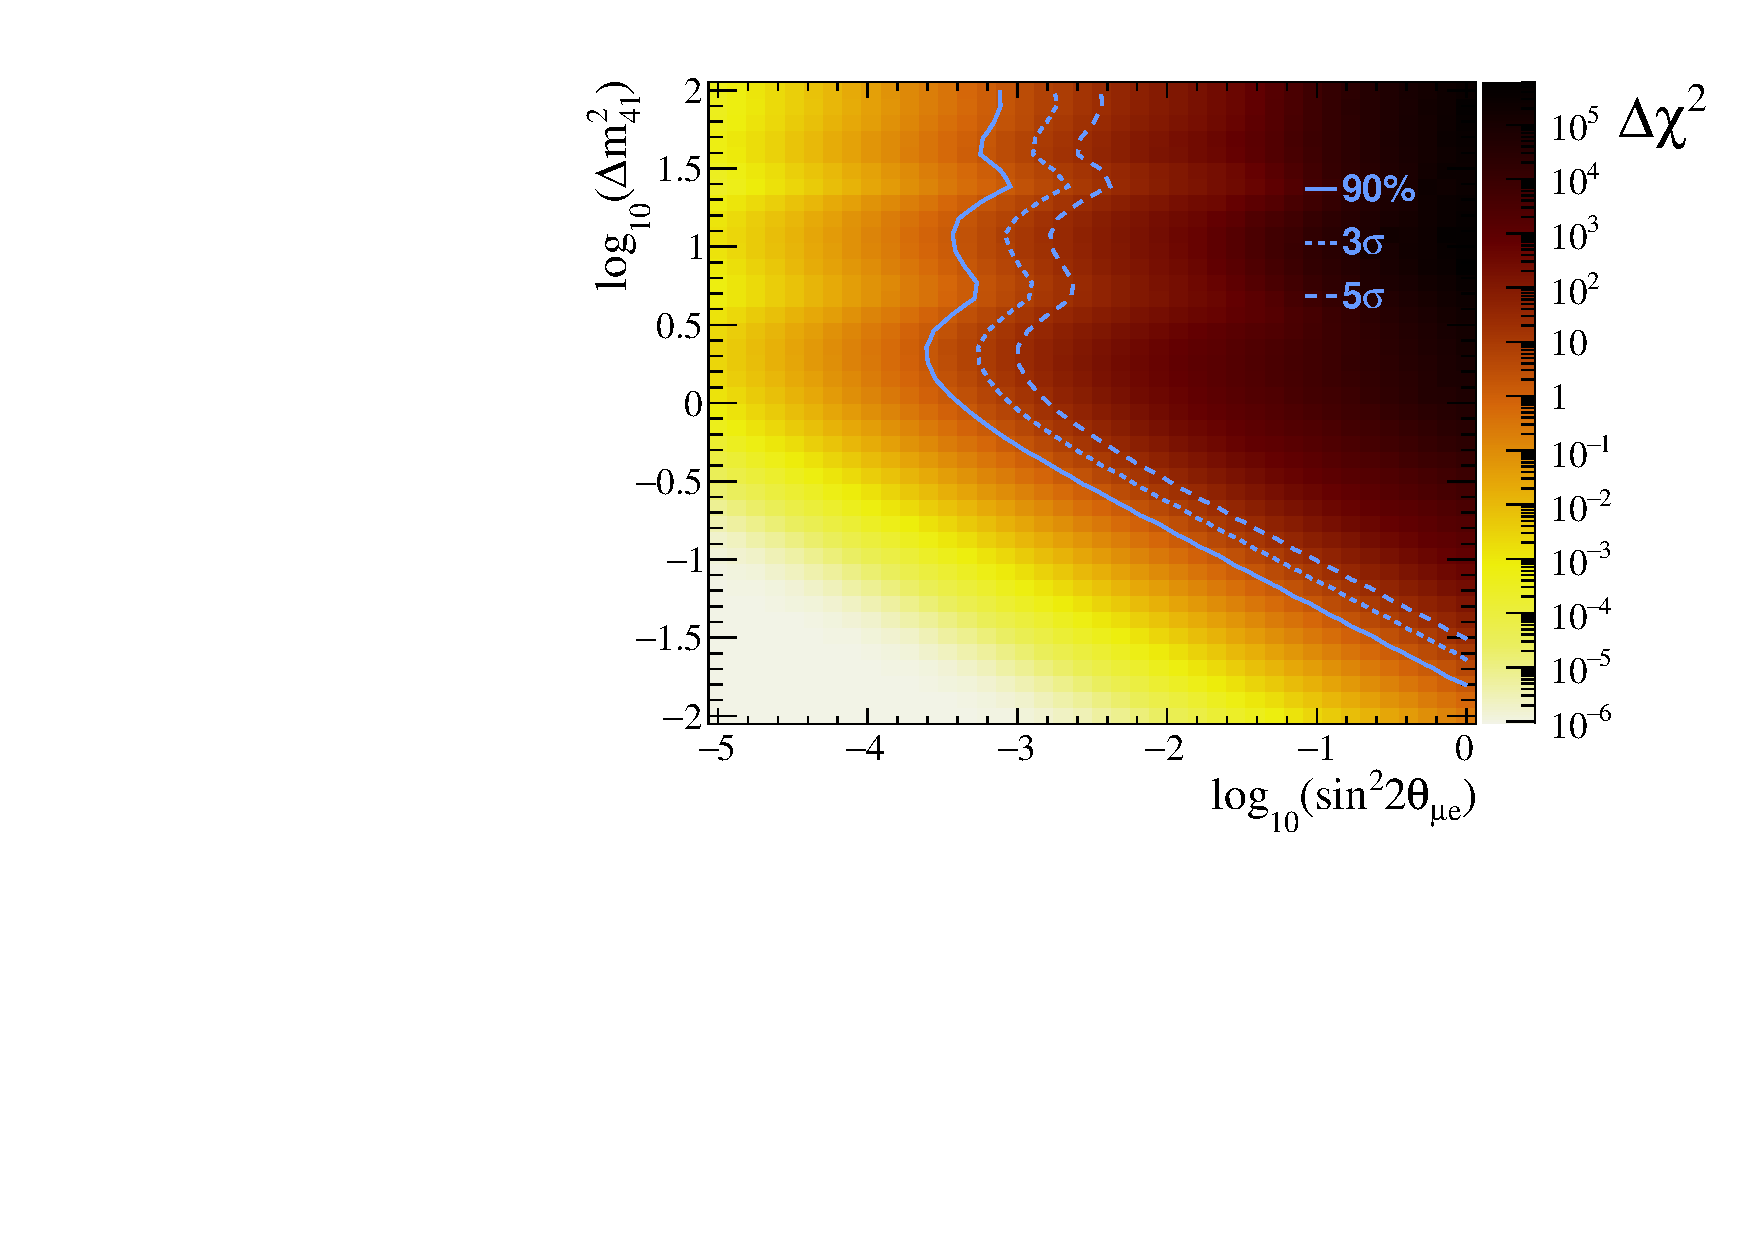
\includegraphics[width = \largefigwidth]{figures-chap6/exclusion_contours/nue_app_03d1_chi2_surface.pdf}
    \caption[\nue appearance contours overlayed on the $\chi^2$ surface.]{The \nue appearance $\chi^2$ surface from fits including flux and interaction systematics. Contours of constant $\chi^2$ values which correspond to 90\%, 3$\sigma$ and 5$\sigma$ confidence levels have been overlayed onto the surface.}
    \label{fig:nue_app_chisq_surface}
\end{figure}

When producing sensitivity contours, the fits may be generated for an individual detector as well as any combination of multiple detectors. The left plot of \FigureRef{fig:nue_sensitivity_detector_contribution} shows the \nue appearance statistical-only sensitivity contours from each individual detector as well as all possible combinations (the black curve labelled "SBN" refers to a contour from combining all three detectors). It can be seen that for large $\Delta m^2_{41}$ (greater than $\sim$5 eV$^2$), that the \gls{sbnd} detector dominates the sensitivity whereas for small $\Delta m^2_{41}$ (less than $\sim$0.7 eV$^2$) the \gls{icarus} detector dominates. It should also be noted that only by combining the fits from all three detectors can the best sensitivities be obtained. Having this multi-detector design is one of the key advantages of the \gls{sbn} program. The right plot of \FigureRef{fig:nue_sensitivity_detector_contribution} is akin to the left one, but with the inclusion of flux and interaction systematics in the fits. Again, the improvements to the sensitivity are highlighted by combining multiple detectors. 

\begin{figure}[h!]
    \centering
    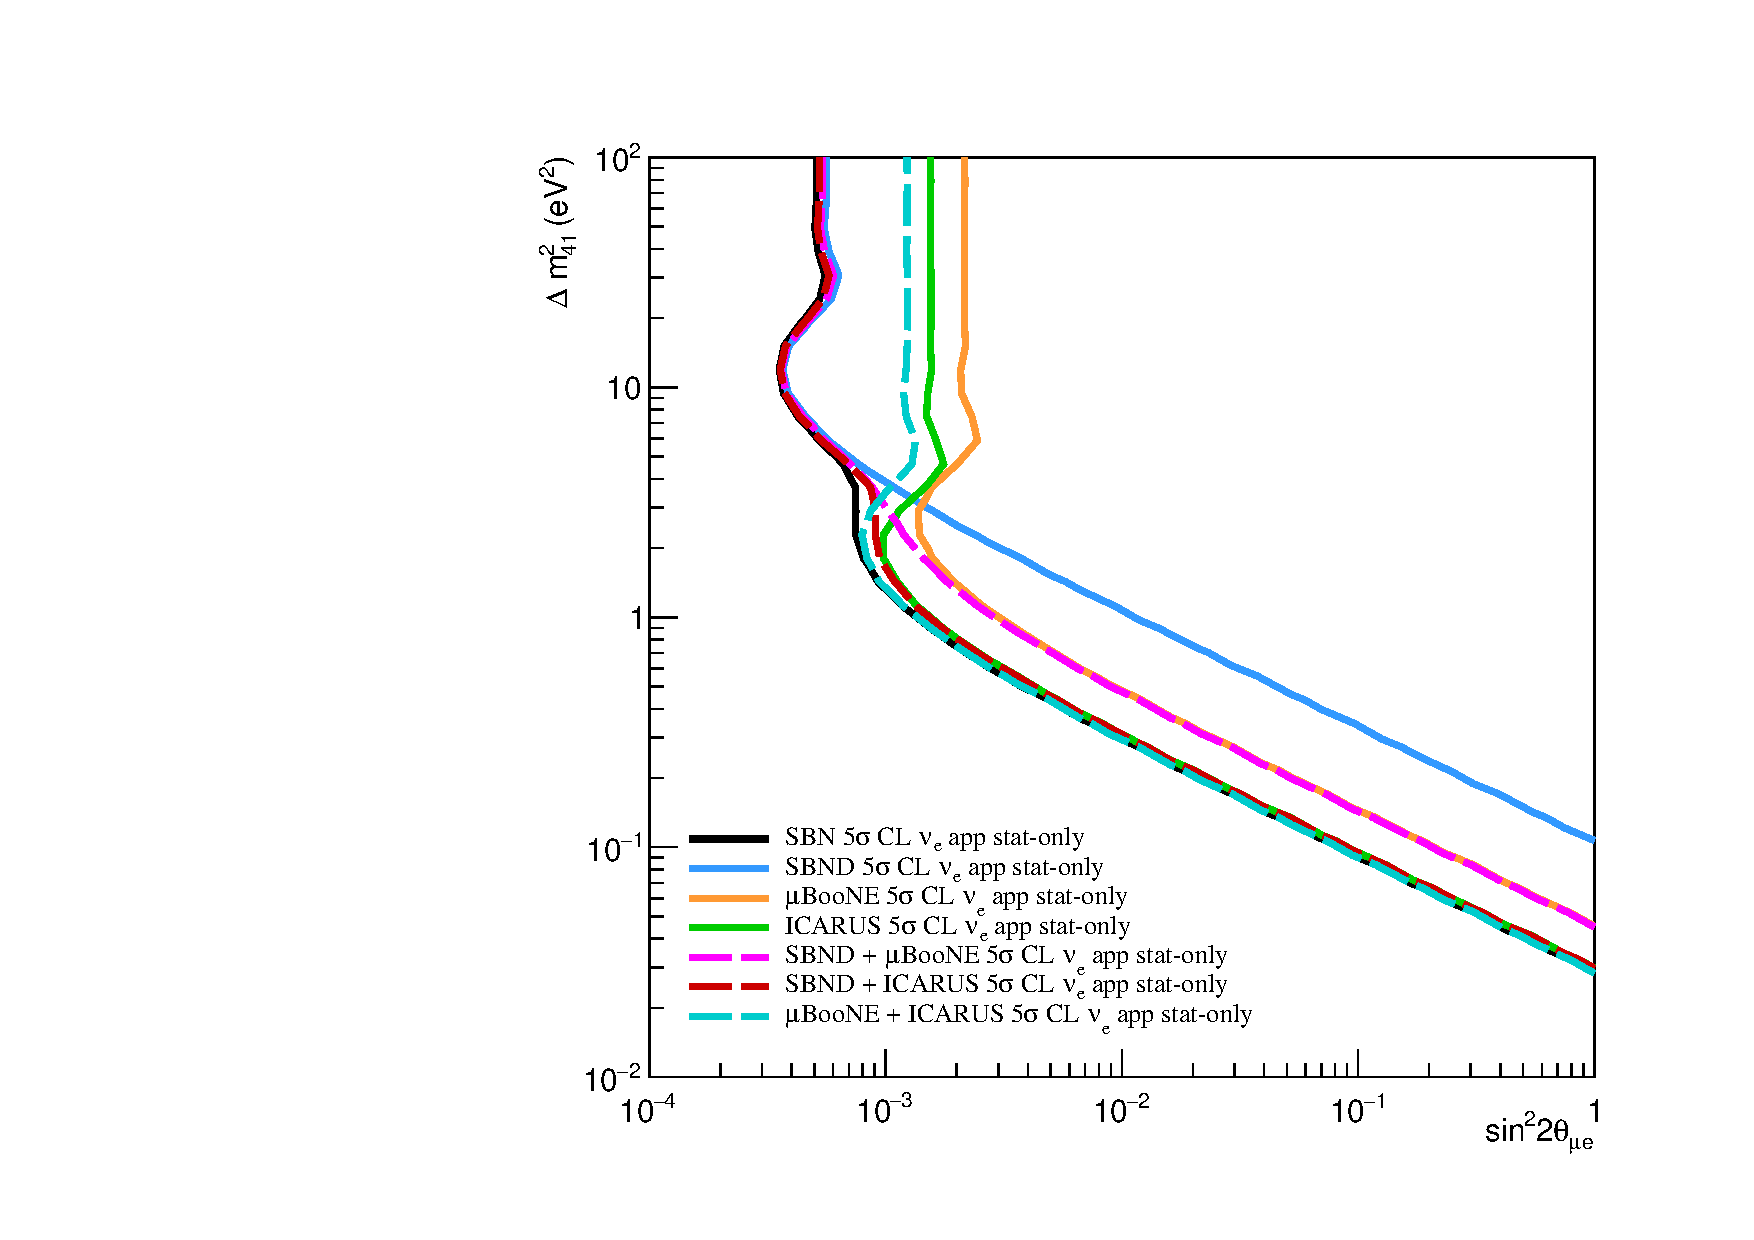
\includegraphics[width = 0.49\textwidth]{figures-chap6/exclusion_contours/nue_app_detector_combinations_stat_only.pdf}
    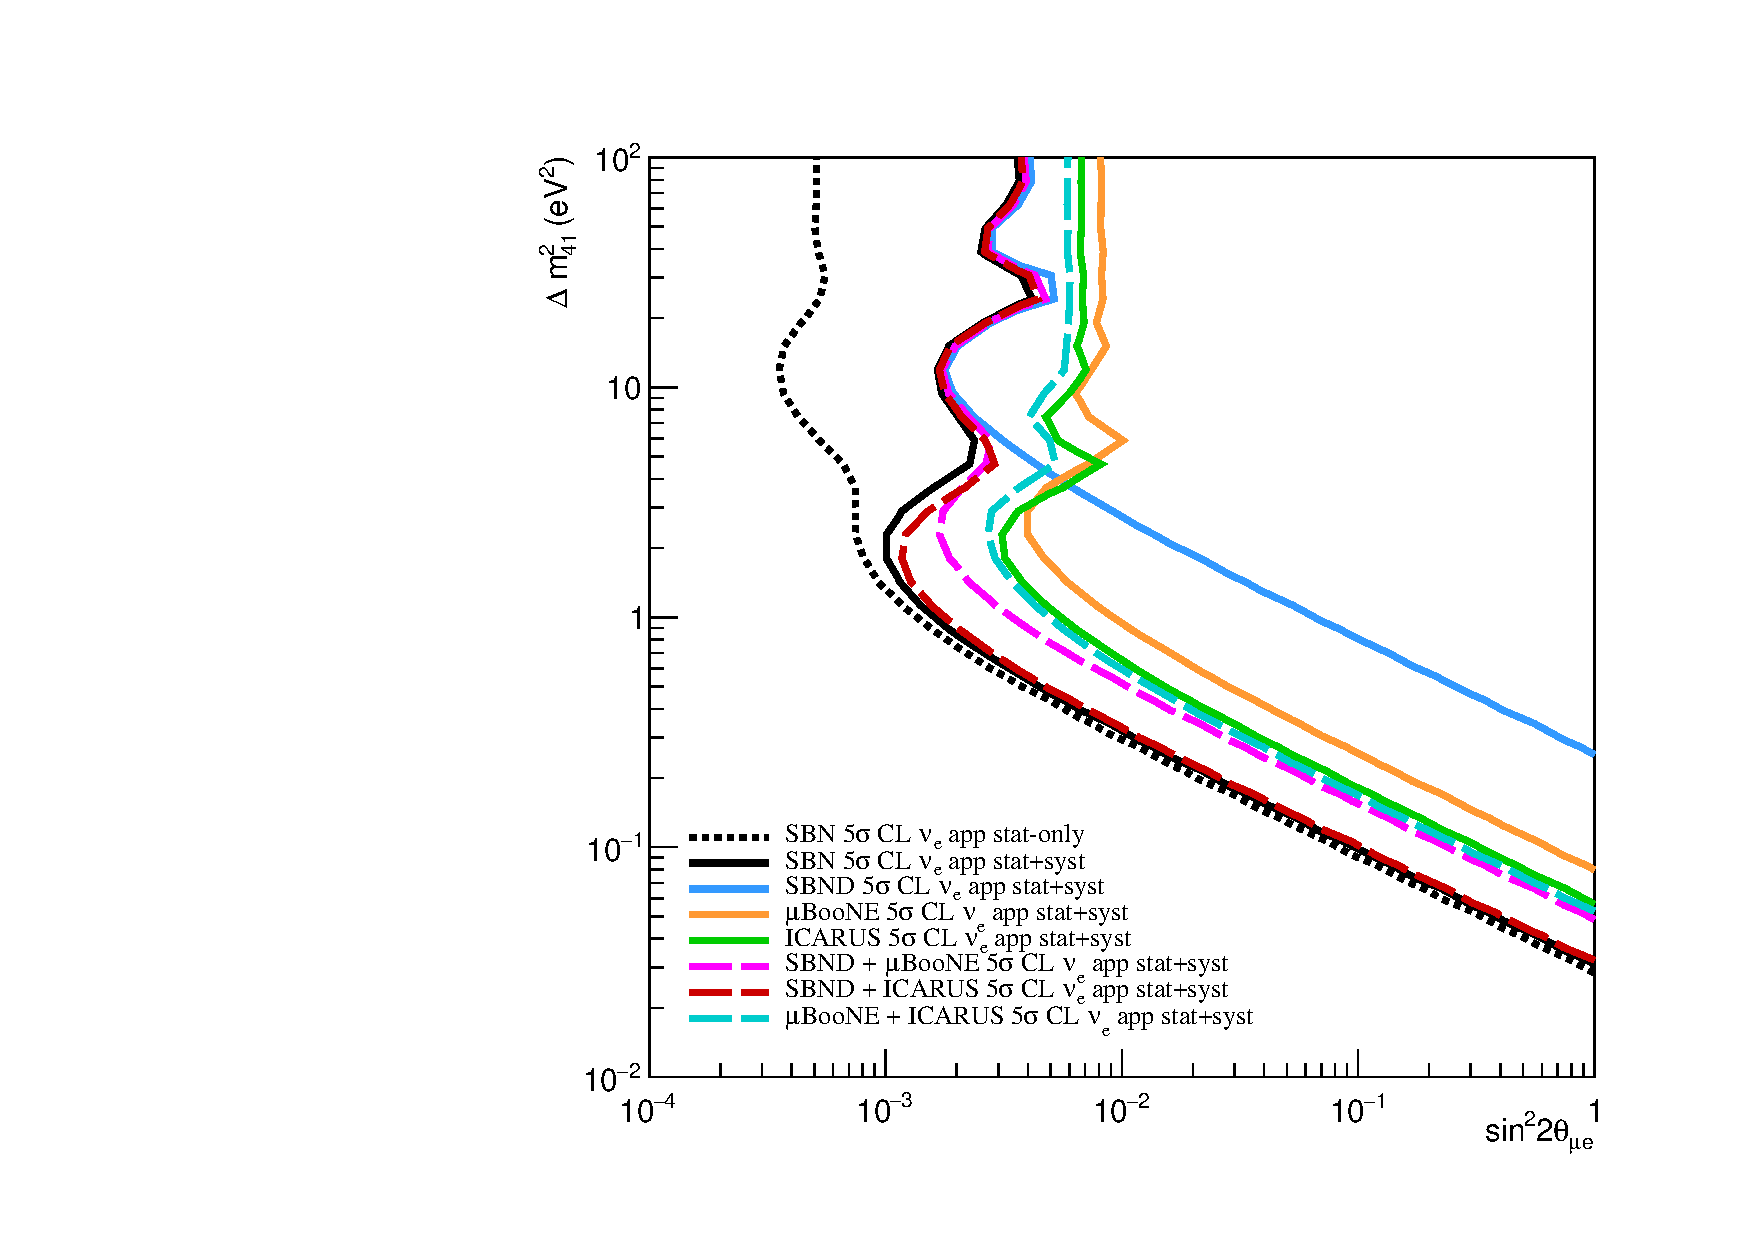
\includegraphics[width = 0.49\textwidth]{figures-chap6/exclusion_contours/nue_app_detector_combinations_stat+syst.pdf}
    \caption[\nue appearance sensitivities from different detector combinations.]{Contributions to the SBN \nue appearance sterile oscillation sensitivity from each detector and combinations of detectors in the SBN program. The statistical-only plots in the left-hand figure show that SBND is most sensitive to the region $\Delta m_{41}^{2} >$ $\sim$3 eV$^{2}$and ICARUS is most sensitive to $\Delta m_{41}^{2} <$ $\sim$3 eV$^{2}$. The right-hand figure includes flux and interaction systematic parameters and highlights the considerable improvement in the oscillation sensitivity when including multiple detectors in the fits.}
    \label{fig:nue_sensitivity_detector_contribution}
\end{figure}

The previously discussed figures showing contours including systematic uncertainties simply included all the flux and interaction systemtatics outlined in \SectionRef{sec:syst_uncertainties}, however, it is possible to apply only certain systematics at a time. The left plot of  \FigureRef{fig:nue_app_syst_group_sensitivities} shows the reduction in sensitivity when individually applying the flux, proposal interaction, modern interaction and all the interaction systematics compared to the statistical only case. This allows for the impact of the different systematic groups to be assessed. The right hand plot of \FigureRef{fig:nue_app_syst_group_sensitivities} shows the ratio of the exclusion contours to the statistical only case. This gives a clearer measure of the impact on the sensitivity in $\sin^2{2\theta_{\mu e}}$ space. It follows that the interaction systematics have the biggest impact on the sensitivity which in turn are dominated by the modern set of interaction parameters. The proposal set of interaction parameters have the smallest impact with the magnitude of the impact from the flux parameters being somewhere in between the two sets of interaction parameters. 

\begin{figure}[h!]
    \centering
    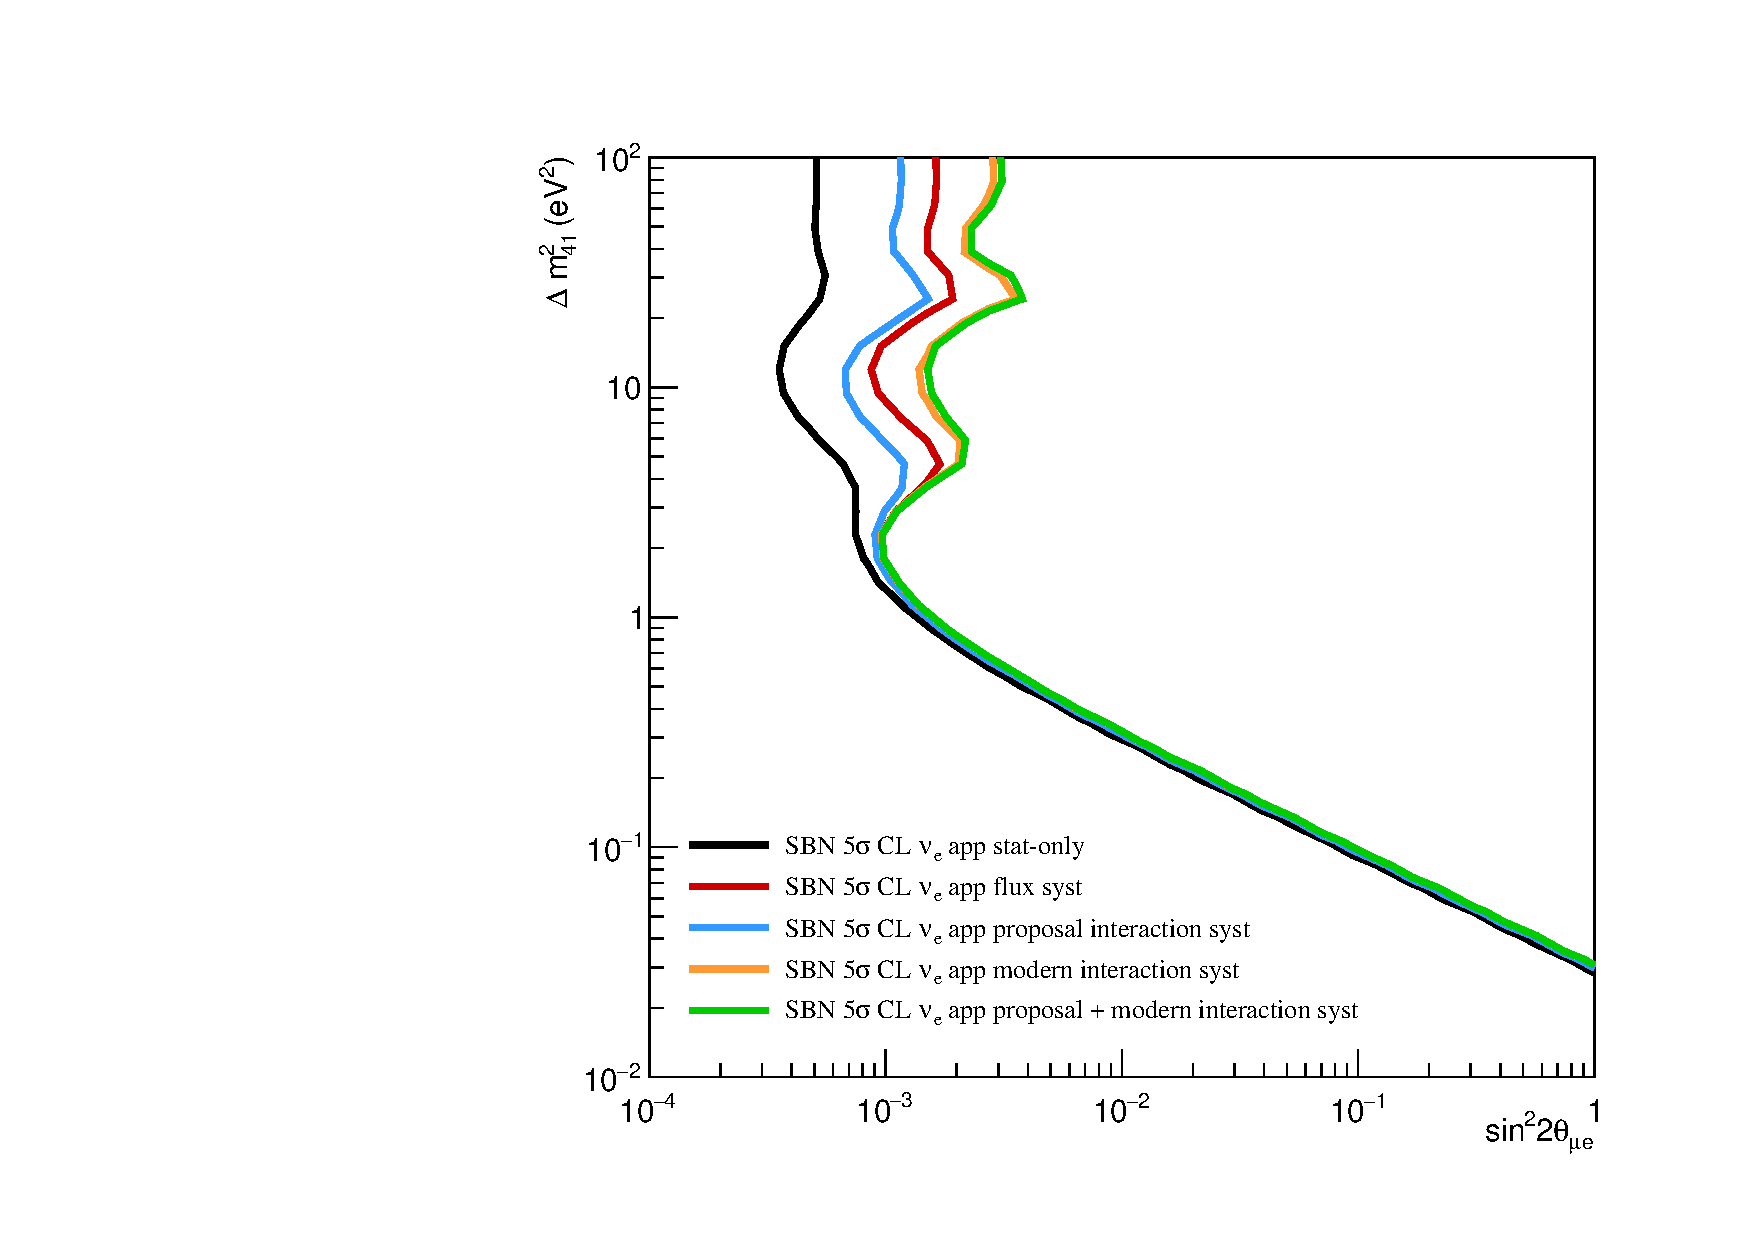
\includegraphics[width = 0.49\textwidth]{figures-chap6/exclusion_contours/nue_app_syst_groups.pdf}
    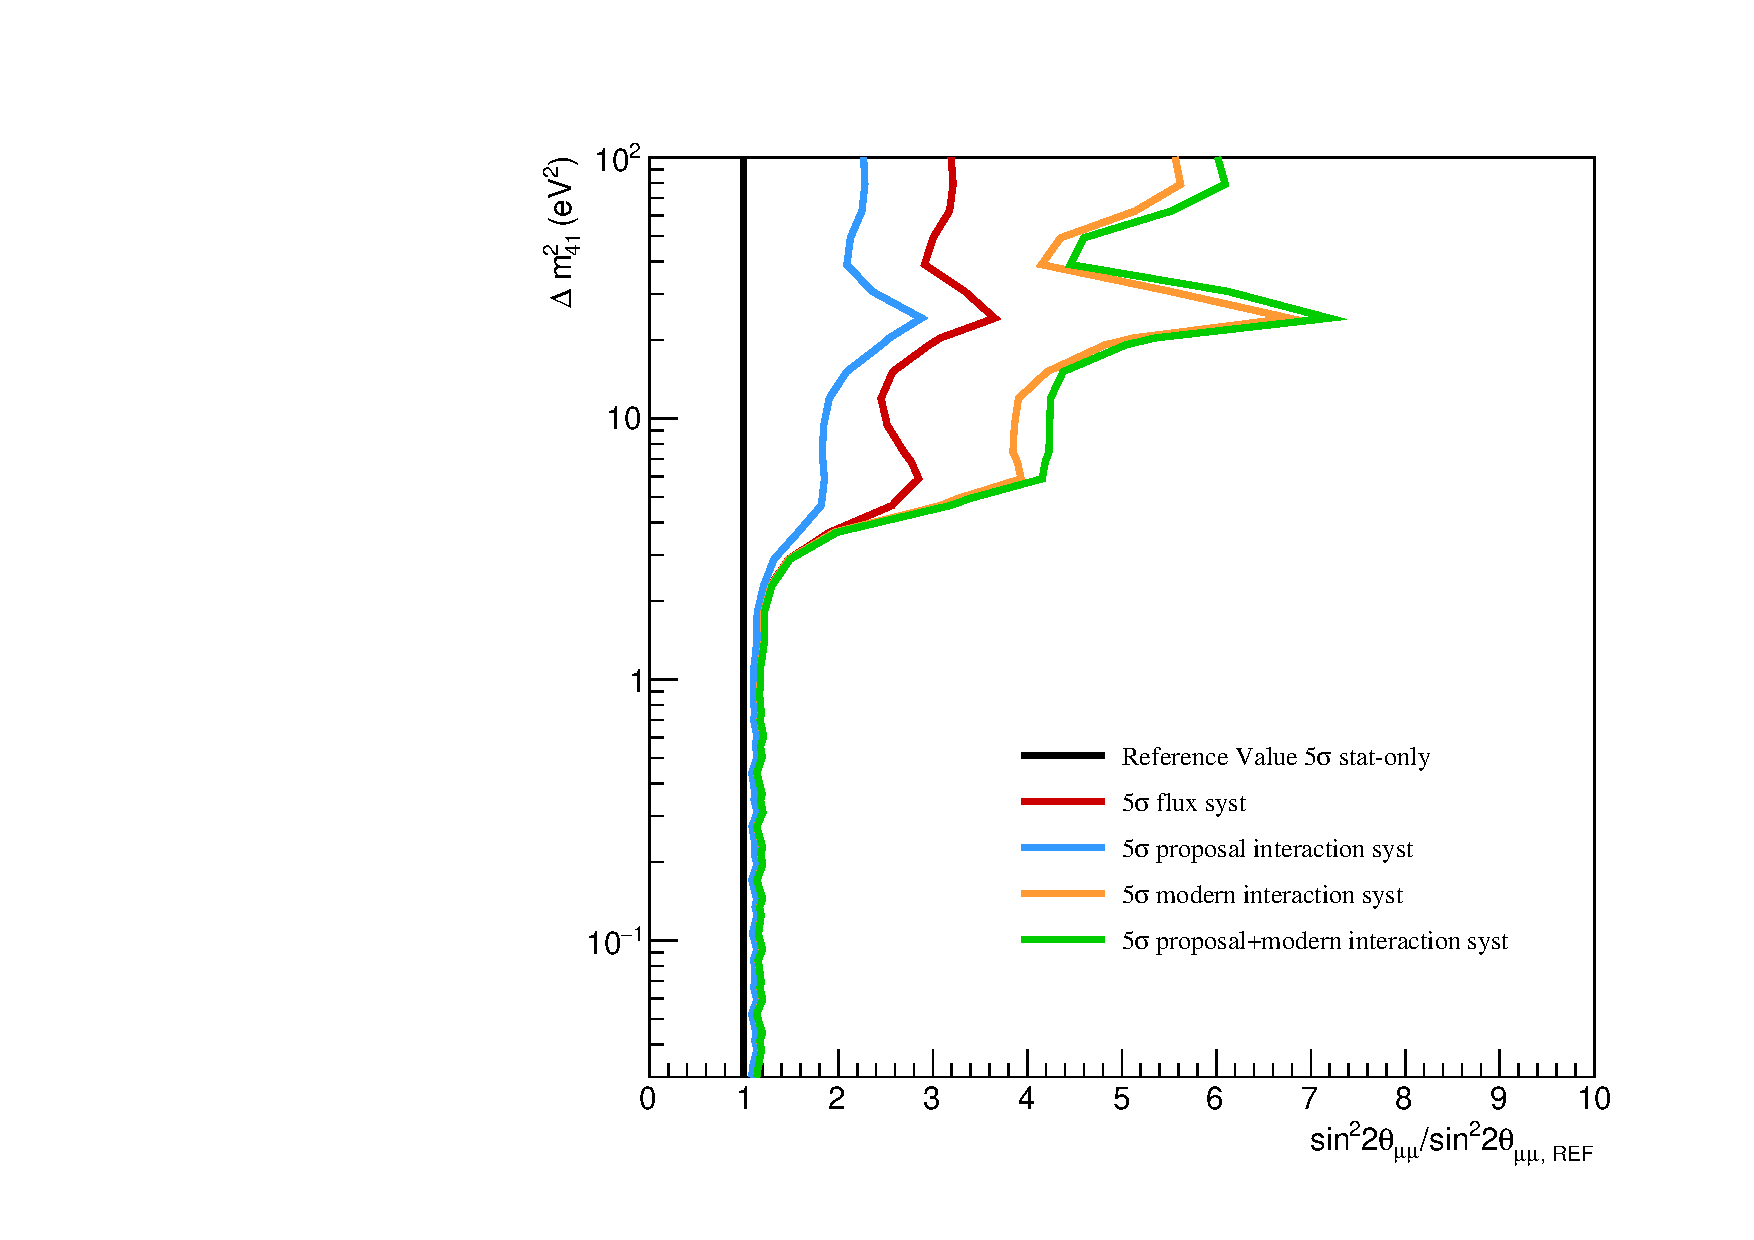
\includegraphics[width = 0.49\textwidth]{figures-chap6/exclusion_contours/nue_app_syst_groups_ratios.pdf}
    \caption[Impact of the different systematic parameter groups on the \nue appearance sensitivity.]{The left plot shows the reduction in sensitivity from the stat-only contour when including each set of systematic parameters in the fits and was produced by the VALOR fitting framework. The right plot shows the relative location of each systematic contour in $\sin^{2}2\theta_{\mu e}$ space, with respect to the statistical-only case for the active region of $\Delta m_{41}^{2}$ phase space.}
    \label{fig:nue_app_syst_group_sensitivities}
\end{figure}

The complete \nue appearance exclusion sensitivities and allowed regions for both the statistical only case and with the inclusion of flux and interaction systematics are shown in \FigureRef{fig:nue_app_global_sensitivity} for the entire \gls{sbn} program alongside external limits from the \gls{lsnd} and \gls{karmen} experiments \cite{LSND_KARMEN_nue_app_contour}. For comparison purposes, it should be noted that the contours produced for the \gls{sbn} program are at the $5\sigma$ confidence level whereas the results from both \gls{lsnd} and \gls{karmen} are at the 99\% confidence level. The results from \gls{sbn} shows an improvement over the \gls{karmen} results for essentially all $\Delta m^2_{41}$ values and the allowed region is largely consistent with the \gls{lsnd} result. 


\begin{figure}[h!]
    \centering
    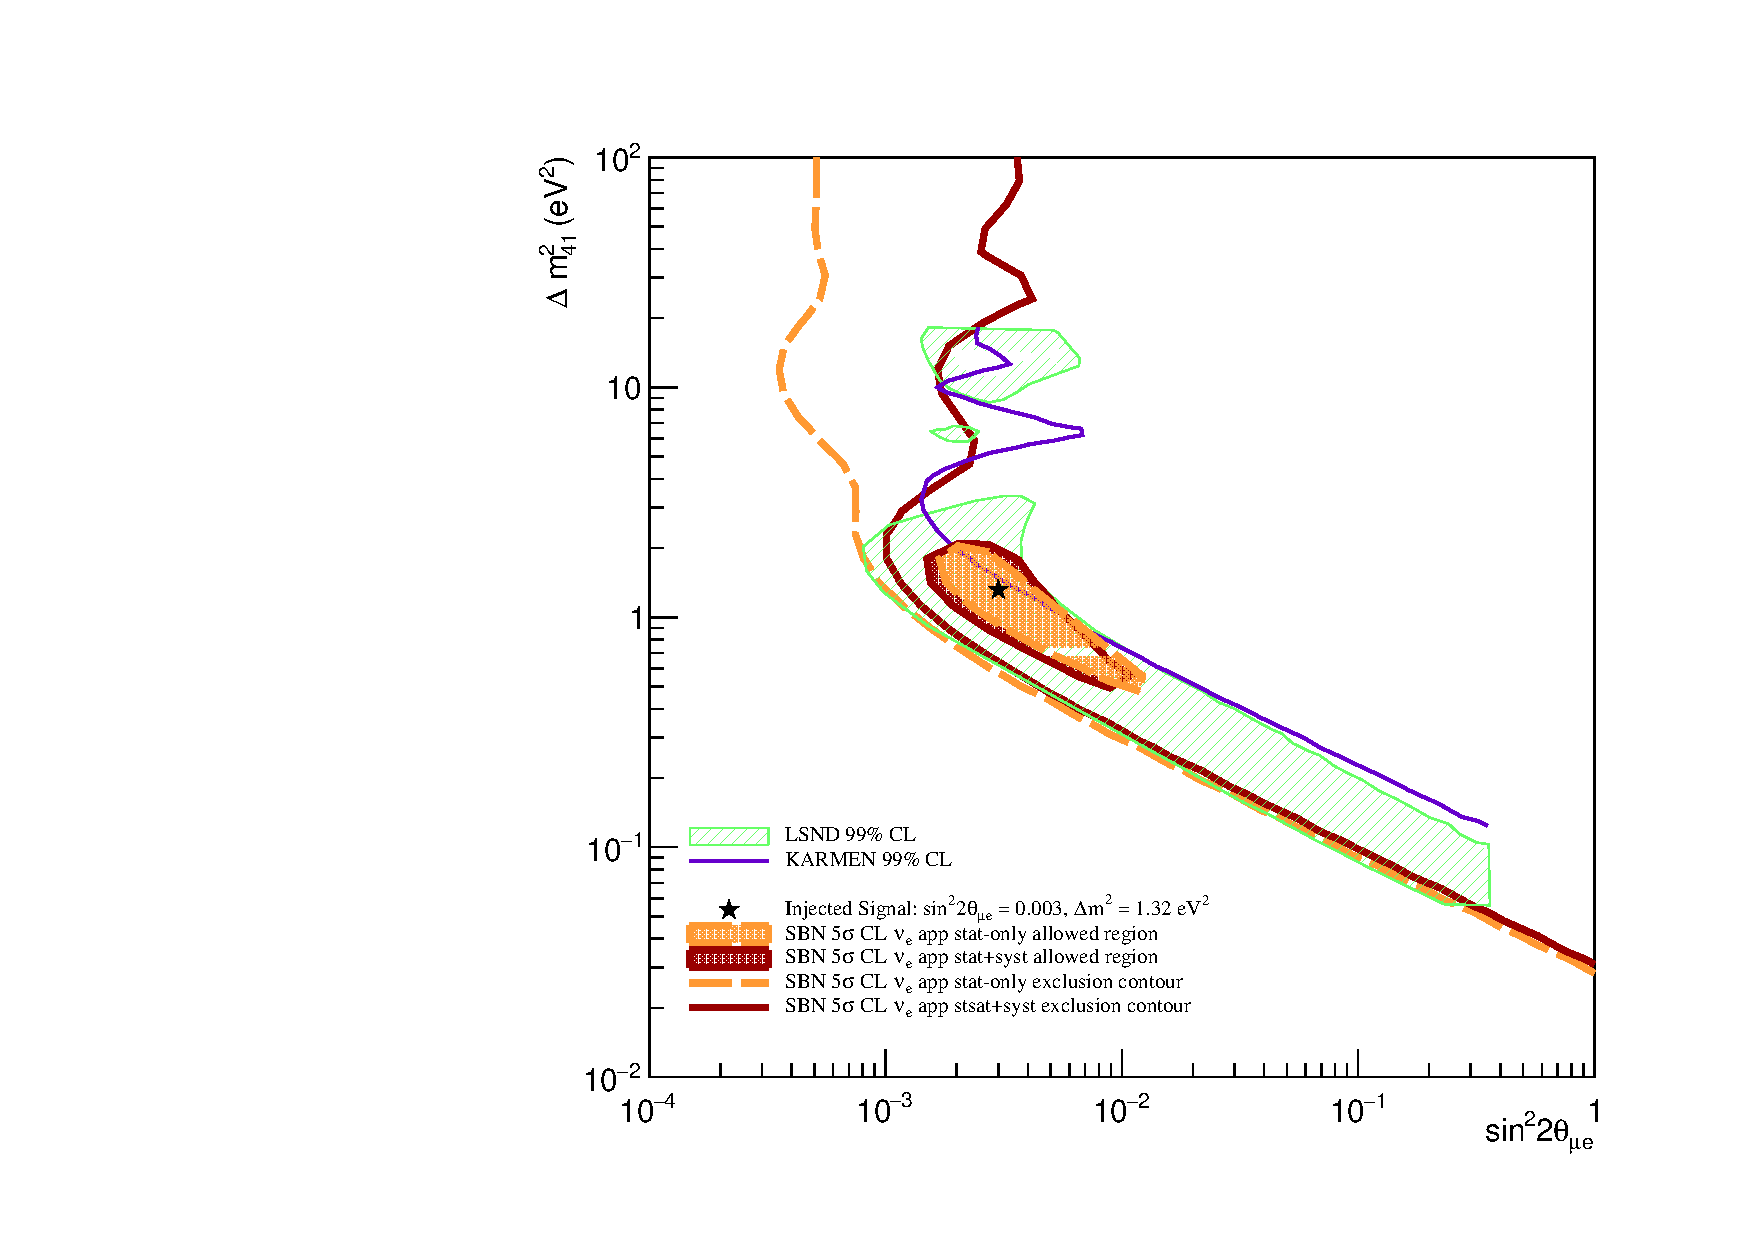
\includegraphics[width = \largefigwidth]{figures-chap6/overlays/valor_overlays_nue_app.pdf}
    \caption[\nue appearance contours with external limits.]{\nue appearance exclusion contours and allowed regions for the stat only case and with flux and interaction systematic uncertainties included. External limits from the \gls{lsnd} and \gls{karmen} experiments have been overlayed \cite{LSND_KARMEN_nue_app_contour}. (The confidence intervals for each contour are shown in the legend and it should be noted that those from external limits are not the same as those from the contours produced for the \gls{sbn} program.)}
    \label{fig:nue_app_global_sensitivity}
\end{figure}


\clearpage
\subsection{\texorpdfstring{\nue Disappearance Analysis}{nue Disappearance Analysis}}

Mirroring the \nue appearance channel, the \nue disappearance channel observes a reduction in the nominal \nue event rate. This is shown in \FigureRef{fig:nue_disapp_spectra} where the integrated spectrum produced with oscillation parameters $\sin^2{2\theta_{ee}} = 0.4$ and $\Delta m^2_{41} = 3 \text{ eV}^2$ has been overlayed onto the breakdown of the nominal spectrum for each of the three detectors. As is the case for \nue appearance, the oscillation signal is relatively small in \gls{sbnd} whereas both \gls{microboone} and \gls{icarus} observe a much more significant signal. 

\begin{figure}[h!]
  {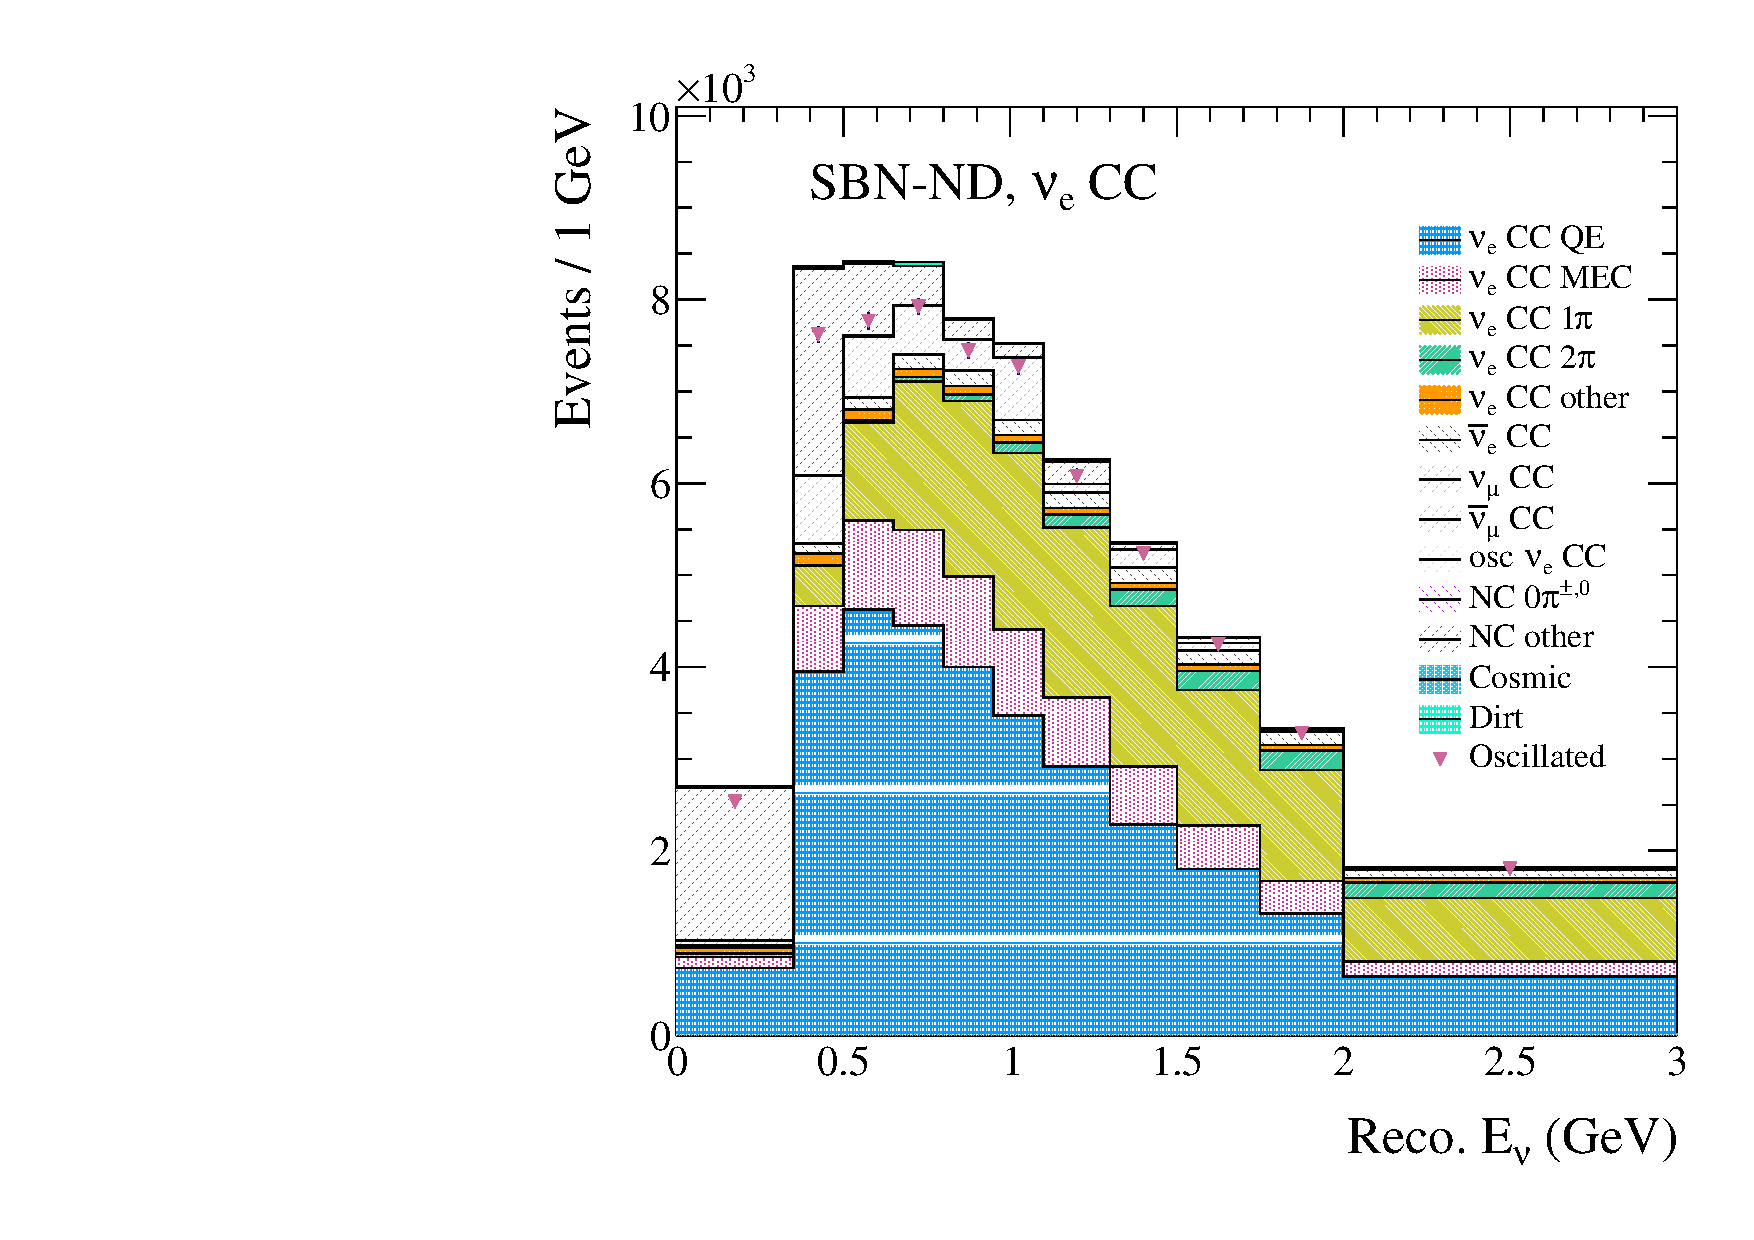
\includegraphics[width=0.49\textwidth]{figures-chap6/spectra/nue_disapp_dmsq_3_sinsq_0.4_overlay_spectrum_sbn_nd_BNB_FHC_0_modes.pdf}}
  {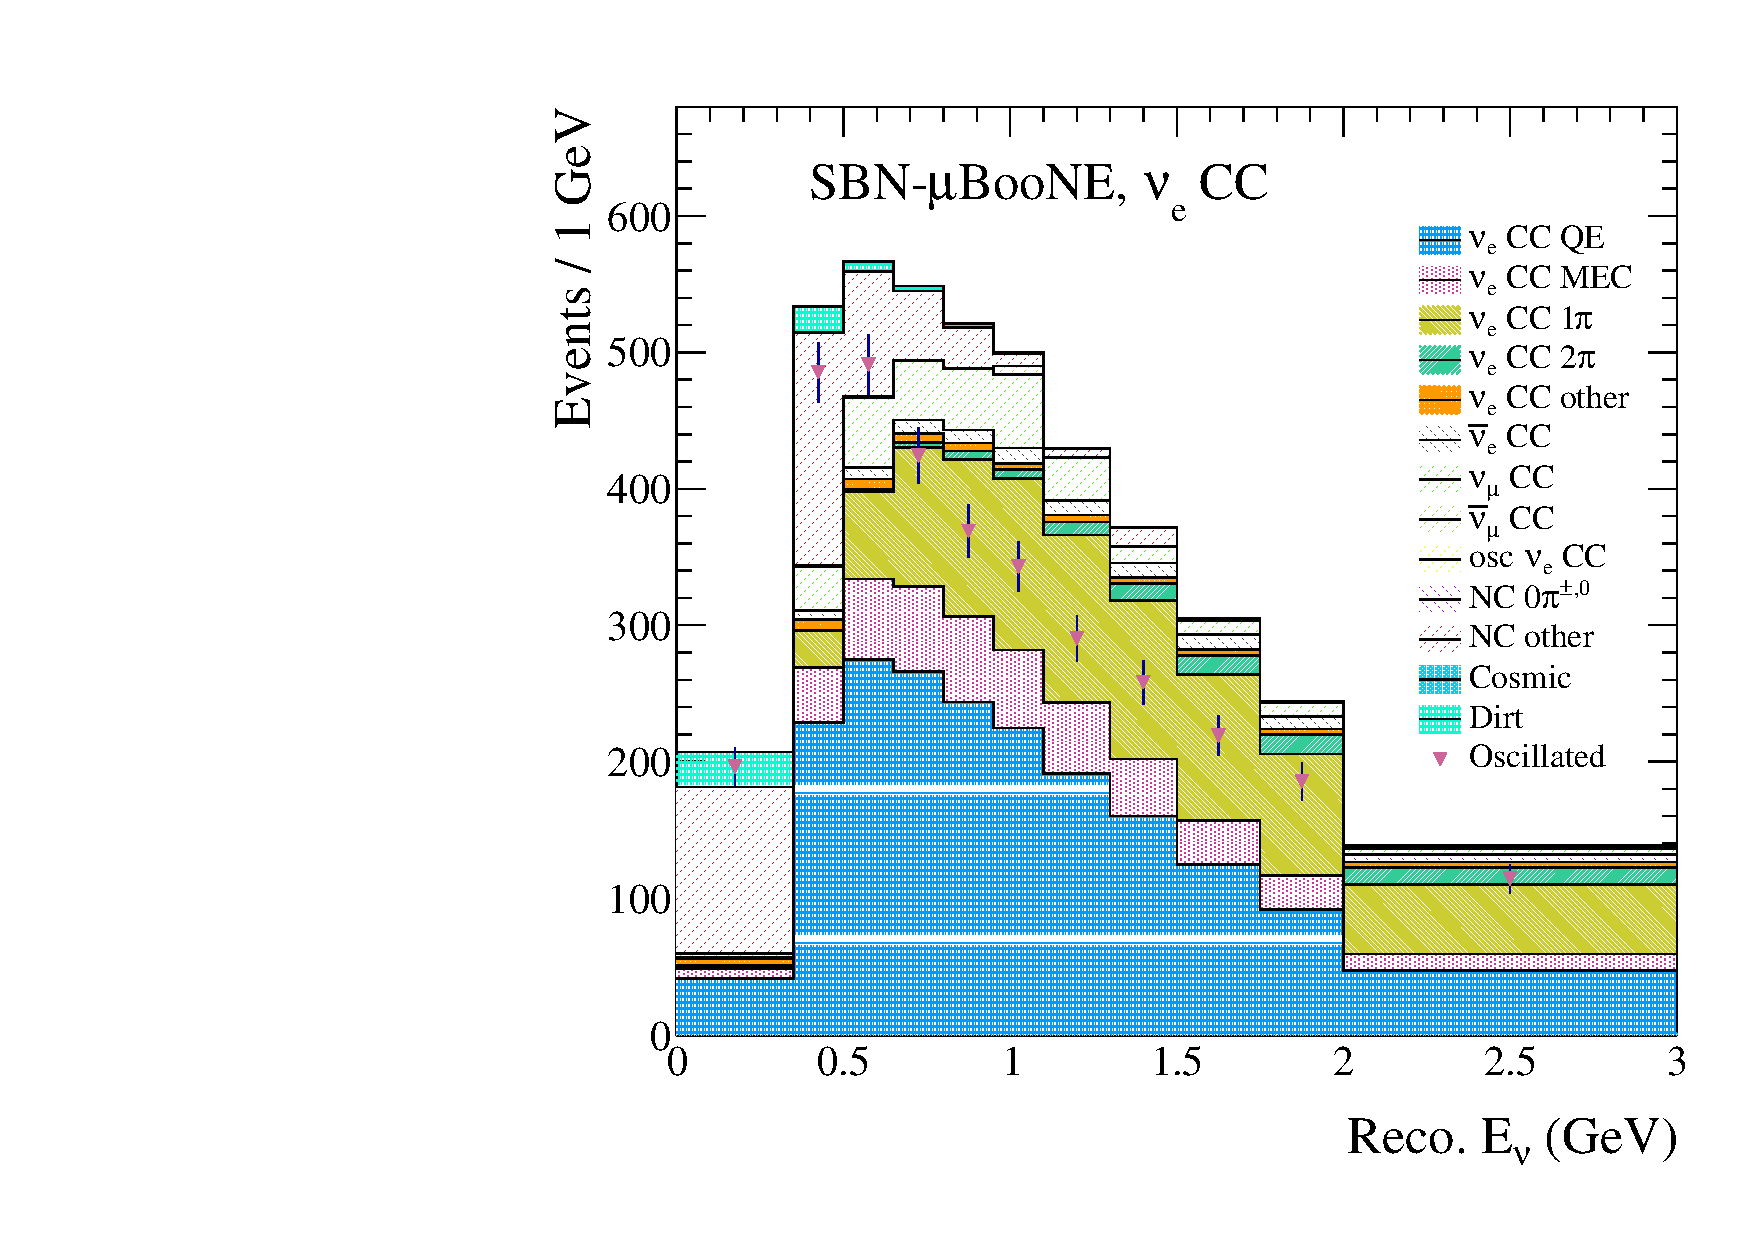
\includegraphics[width=0.49\textwidth]{figures-chap6/spectra/nue_disapp_dmsq_3_sinsq_0.4_overlay_spectrum_sbn_uboone_BNB_FHC_1_modes.pdf}}
  {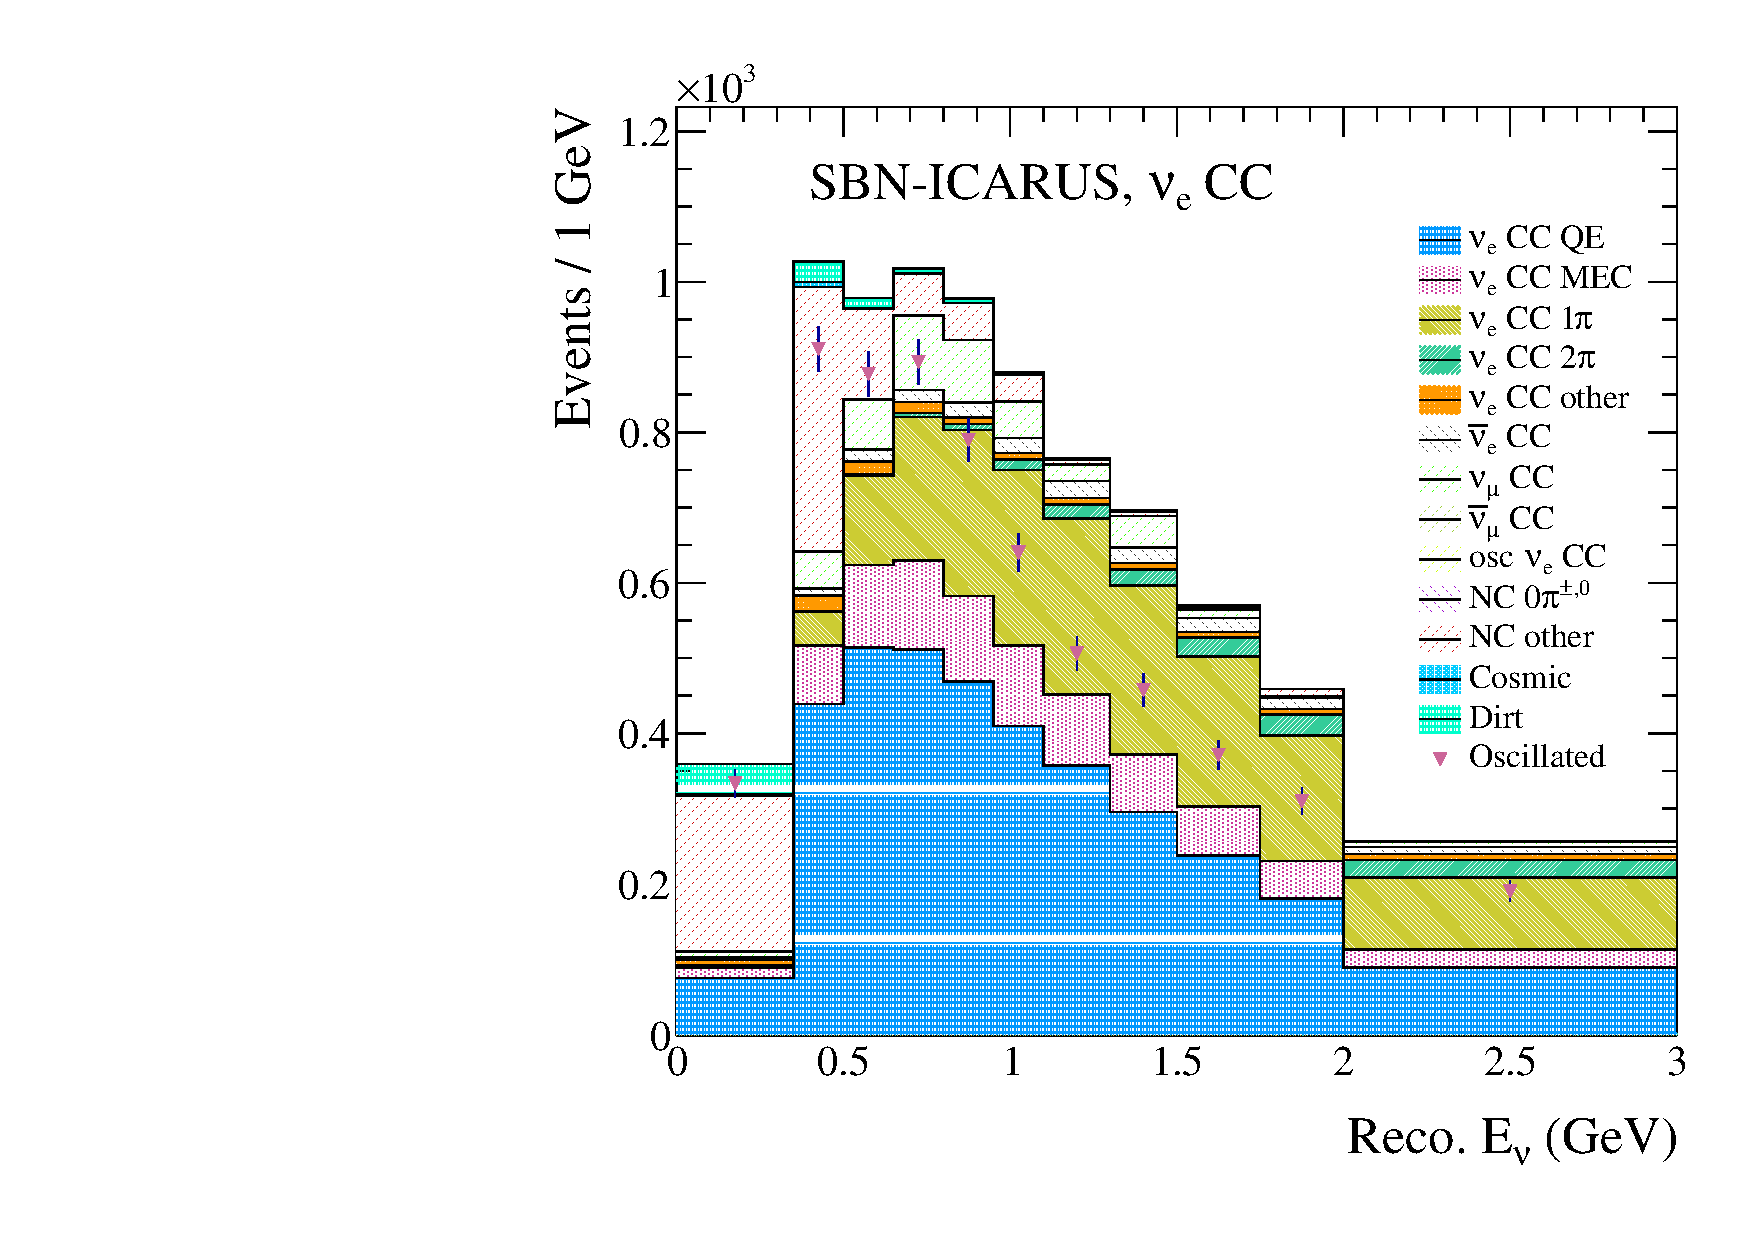
\includegraphics[width=0.49\textwidth]{figures-chap6/spectra/nue_disapp_dmsq_3_sinsq_0.4_overlay_spectrum_sbn_icarus_BNB_FHC_2_modes.pdf}}
  \captionsetup{width=0.49\textwidth}
  \parbox[b]{0.49\textwidth}%
  {
    \caption[SBN \nue disappearance CC inclusive reconstructed neutrino energy spectra with oscillated spectrum overlayed]{The nominal spectra as in \FigureRef{fig:nominal_nue_spectra} but an additional integrated oscillated spectrum with oscillation parameters, $\sin^2{2\theta_{ee}} = 0.4$ and $\Delta m^2_{41} = 3$ eV$^2$ has been overlayed which shows the decrease in event rate.\\\phantom{.}\\\phantom{.}\\\phantom{.}\\}
    \label{fig:nue_disapp_spectra} 
  }
\end{figure}

The top left plot of Figure~\ref{fig:nue_disapp_spectra_ratios} shows the \nue disappearance stat only exclusion contour and allowed region from fits combining all three \gls{sbn} detectors. The injected point \mbox{$\Delta m^2_{41} = 3$~eV$^2$}, $\sin^2{2\theta_{\mu e}} = 0.4$, used when producing the allowed region is shown along with two further points on the exclusion contour at \mbox{$\Delta m^2_{41} = 1$ eV$^2$}, $\sin^2{2\theta_{\mu e}} = 0.29$ and $\Delta m^2_{41} = 100$~eV$^2$, $\sin^2{2\theta_{\mu e}} = 0.085$. \nue disappearance spectra are produced using oscillation parameters corresponding to each of these three points for each of the three SBN detectors. The ratio of each of these oscillated spectra to the nominal for each detector are shown in the the remaining plots in Figure~\ref{fig:nue_disapp_spectra_ratios} and highlight the expected oscillation signal.

\begin{figure}[h!]
    \centering
    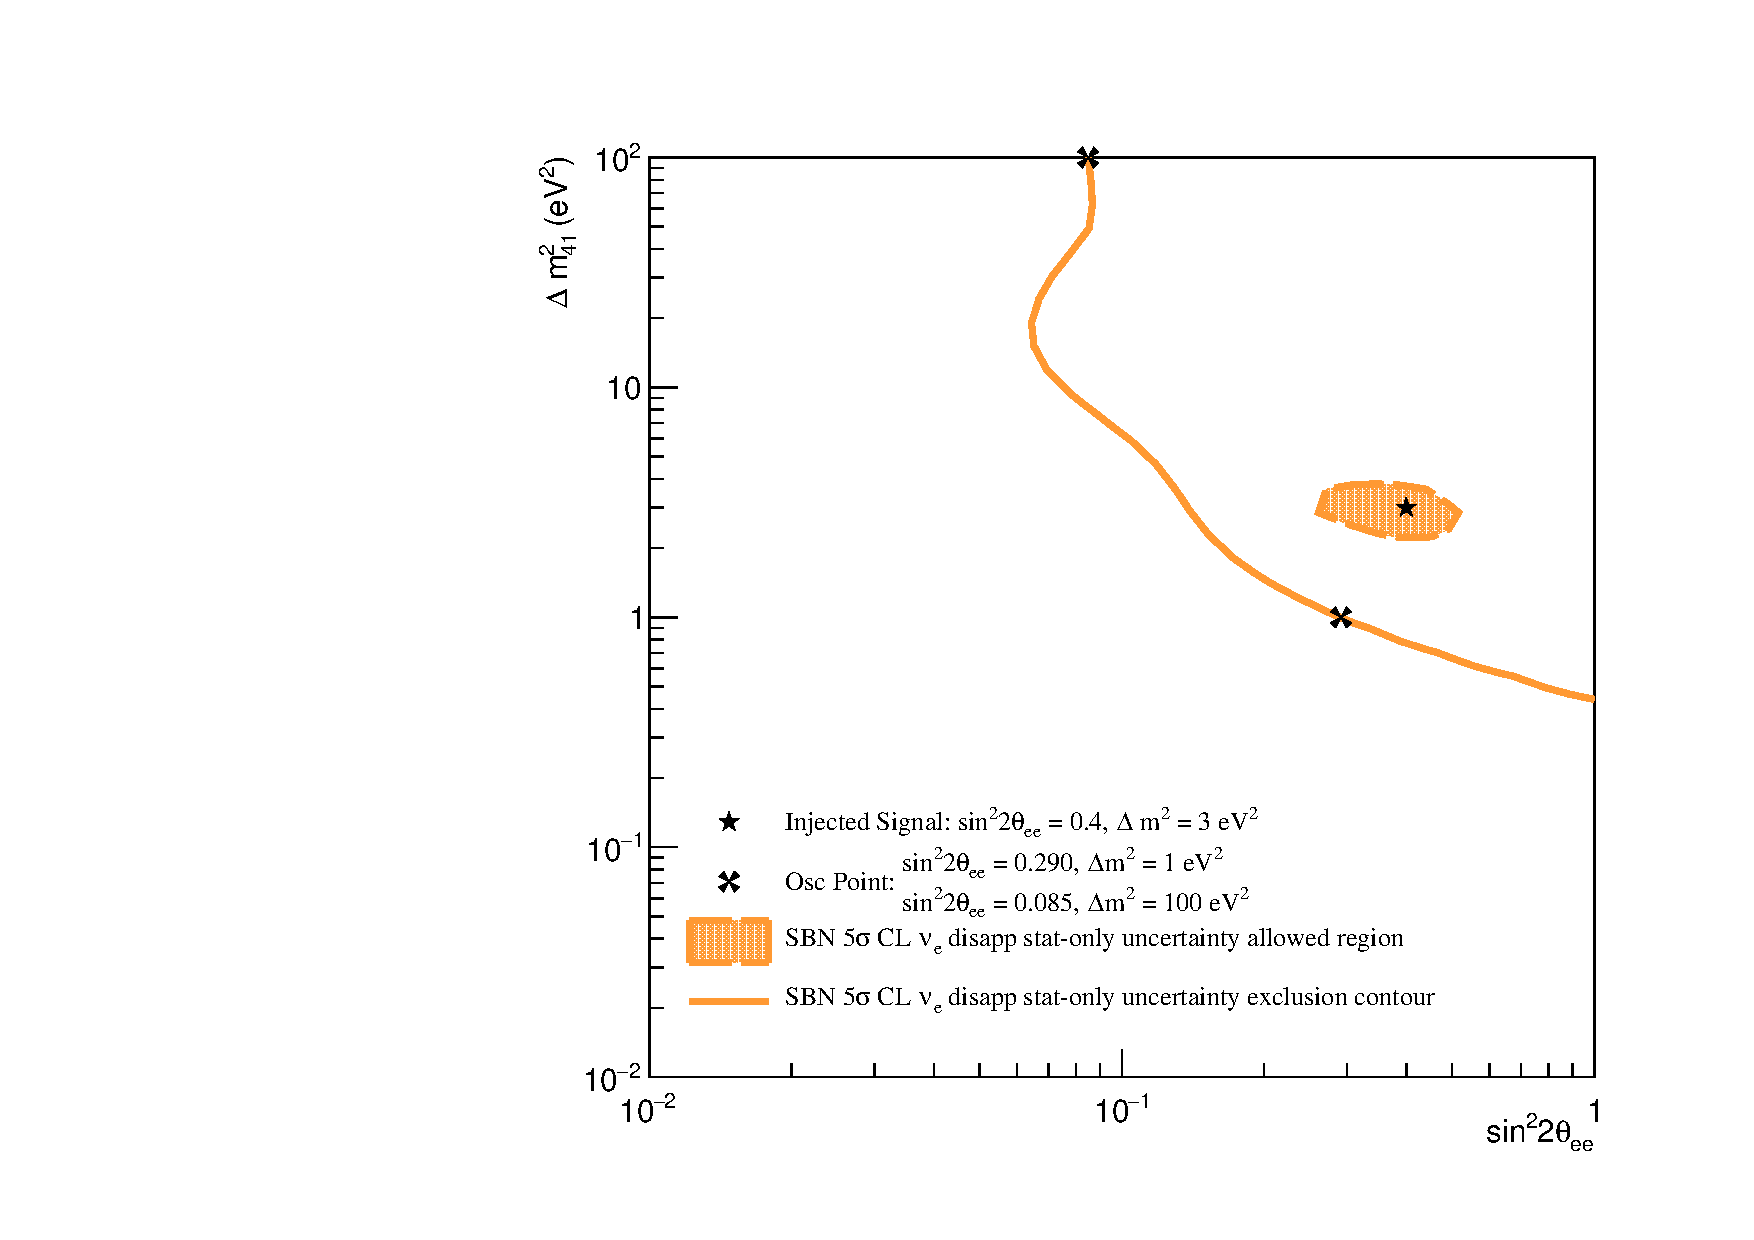
\includegraphics[width = 0.49\textwidth]{figures-chap6/overlays/nue_disapp_stat_osc_markers.pdf}
    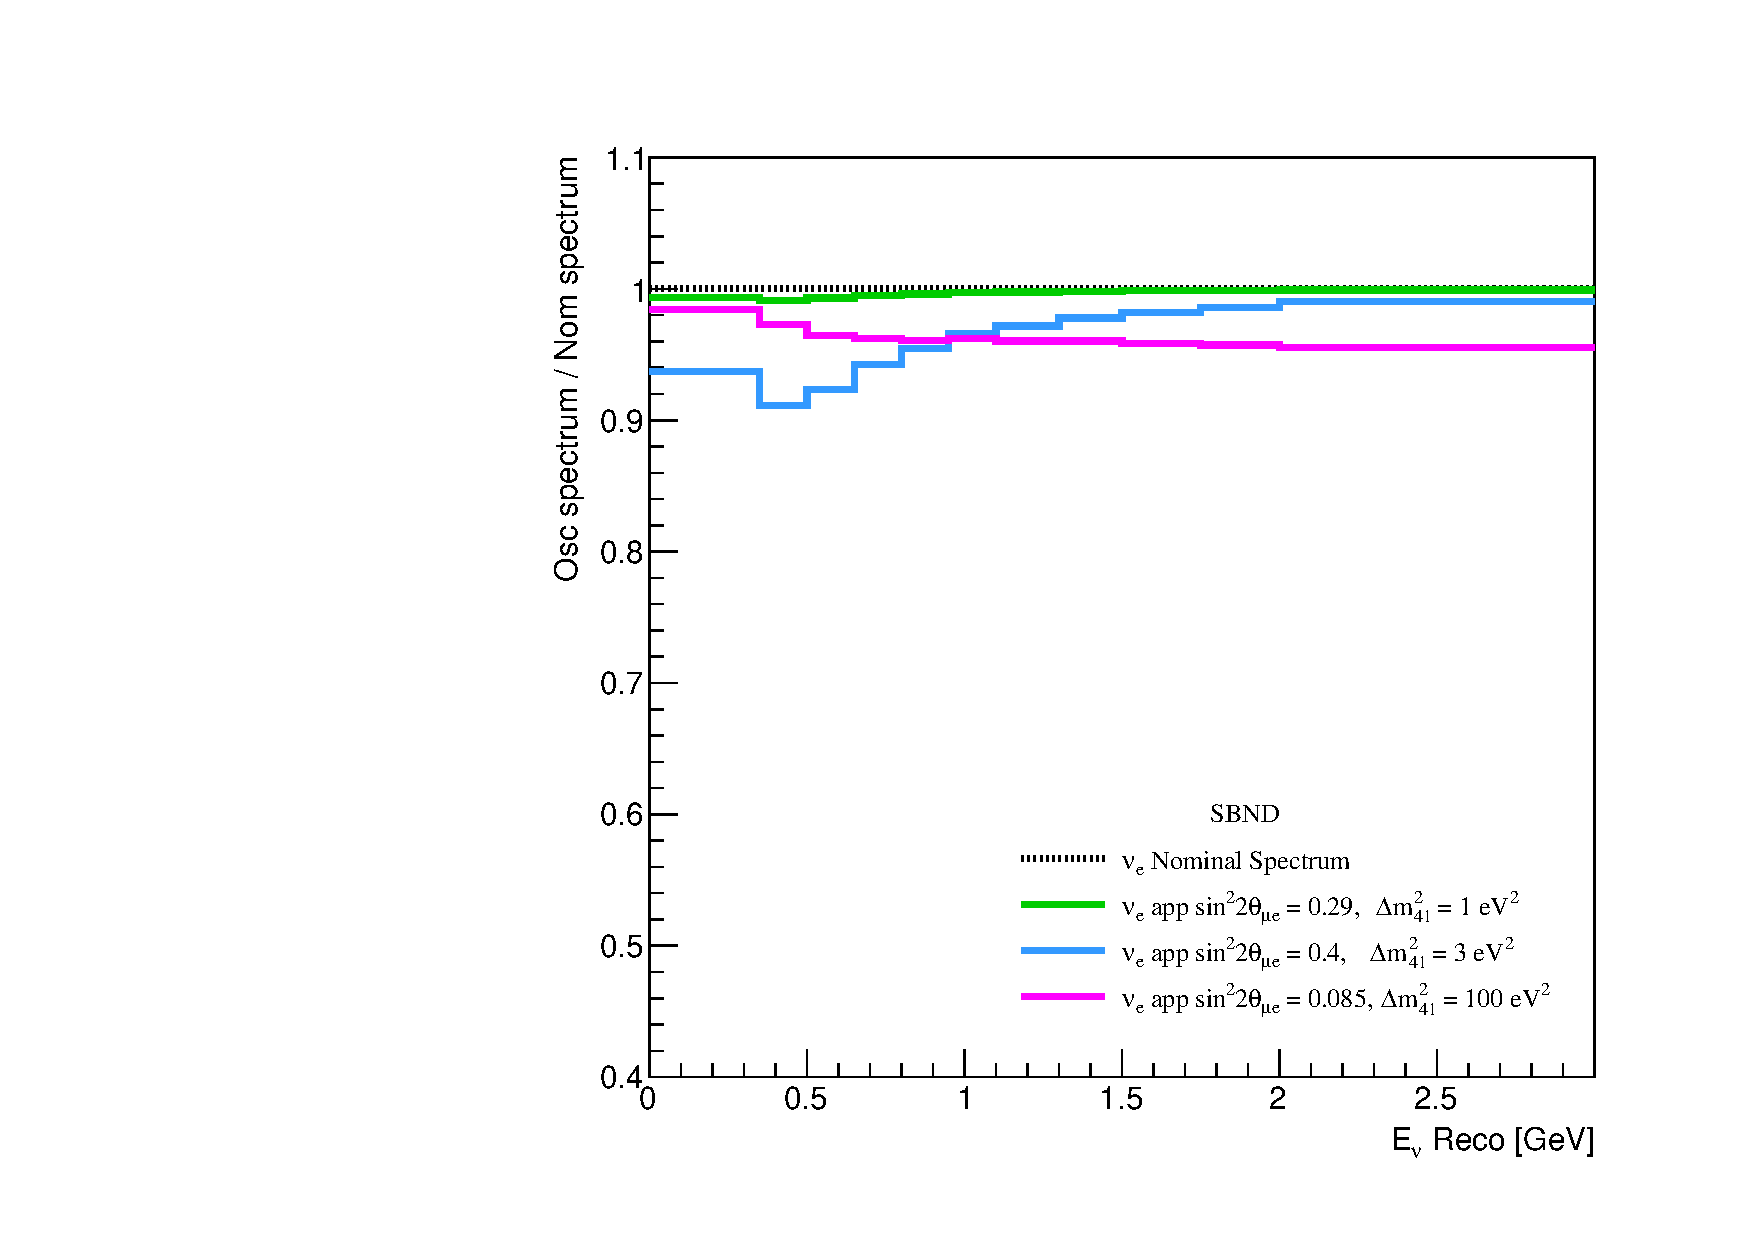
\includegraphics[width = 0.49\textwidth]{figures-chap6/spectra/nue_disapp_spectra_ratio_sbnd.pdf}
    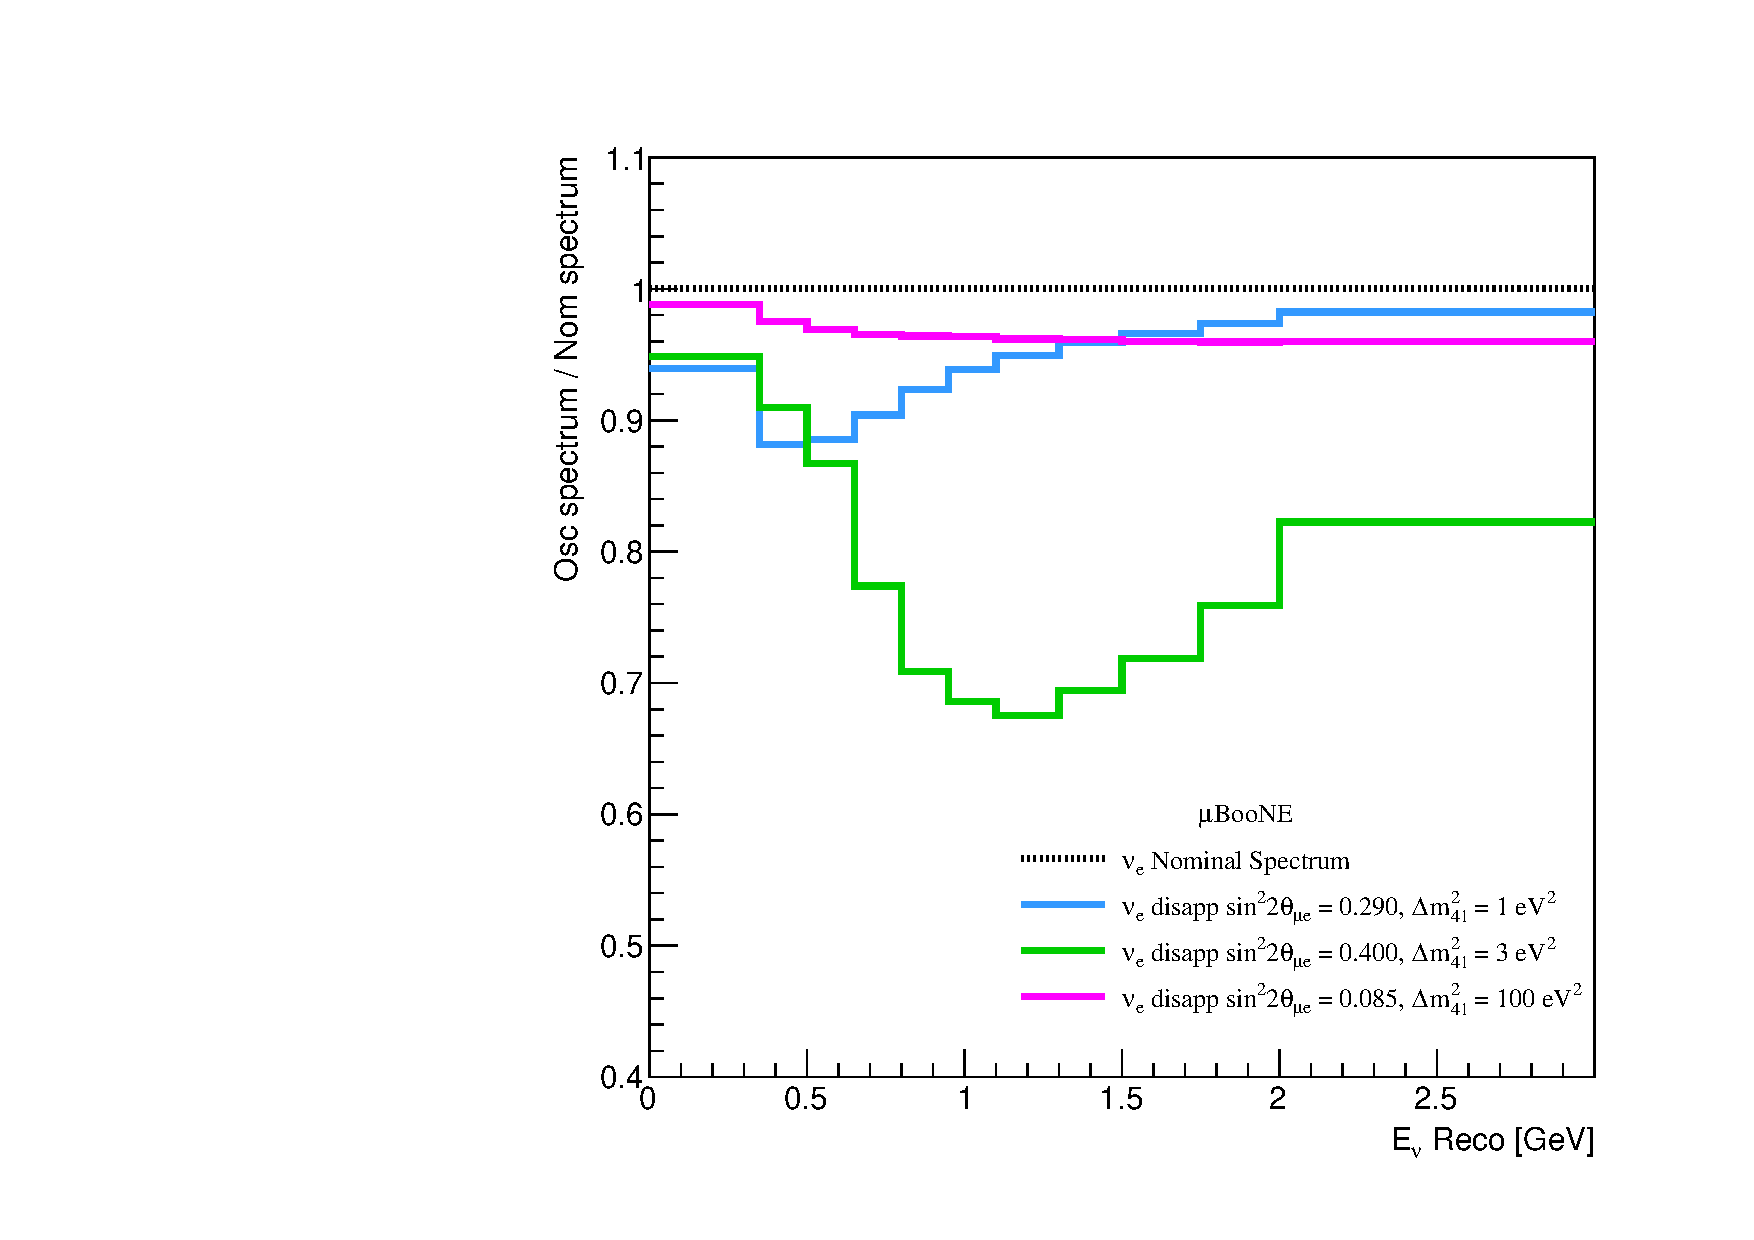
\includegraphics[width = 0.49\textwidth]{figures-chap6/spectra/nue_disapp_spectra_ratio_uboone.pdf}
    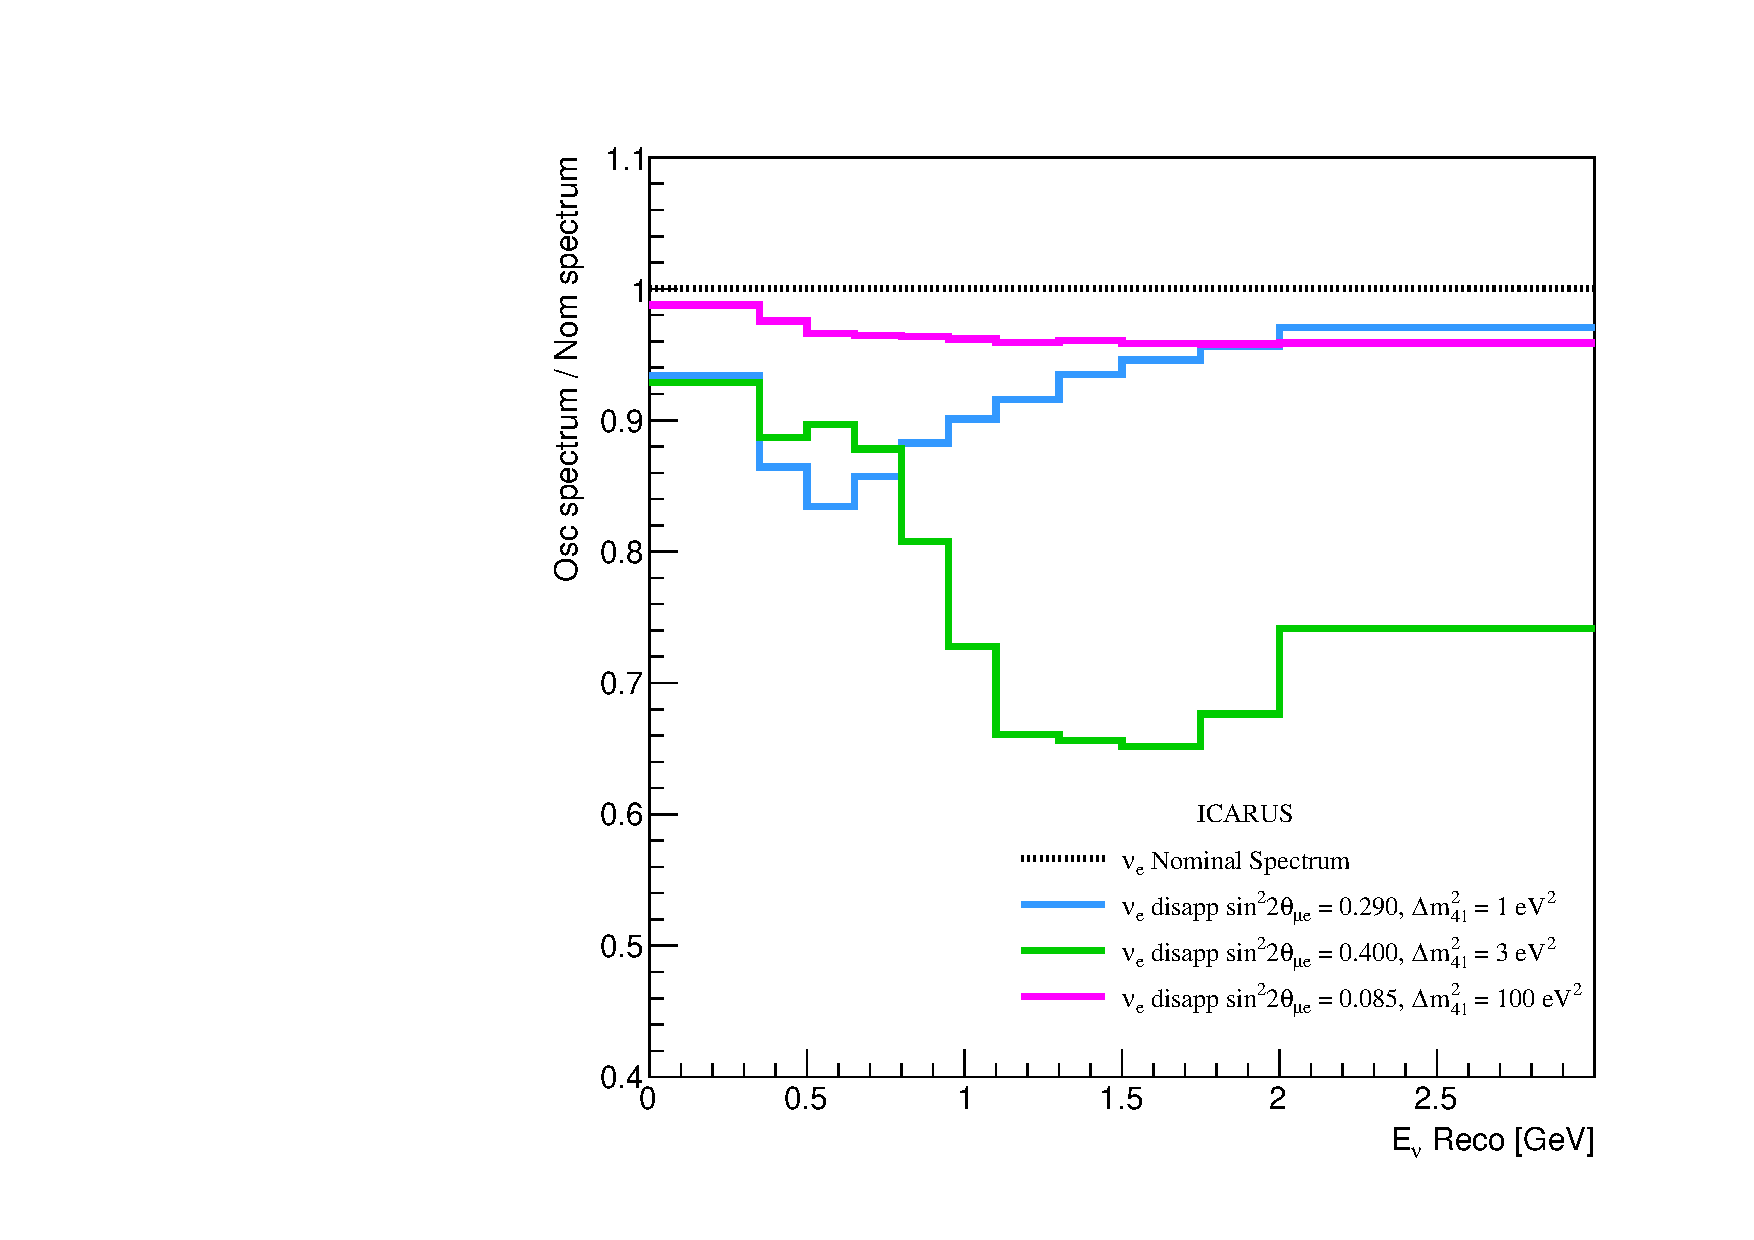
\includegraphics[width = 0.49\textwidth]{figures-chap6/spectra/nue_disapp_spectra_ratio_icarus.pdf}
    \caption[Ratio of \nue disappearance spectra with the oscillation parameters shown on the statistical only contour.]{\nue disappearance stat-only exclusion contour and allowed region. The injected point at $\sin^2{2\theta_{ee}} = 0.4$, $\Delta m^2_{41}$ = 3 eV$^2$ used for the allowed region is shown along with two further points at $\sin^2{2\theta_{ee}} = 0.29$, $\Delta m^2_{41}$ = 1 eV$^2$ and \mbox{$\sin^2{2\theta_{ee}} = 0.085$}, \mbox{$\Delta m^2_{41}$ = 100 eV$^2$} (top left). The ratio of spectra with oscillation parameters corresponding to the three points mentioned versus nominal are shown for \gls{sbnd} (top right), MicroBooNE (bottom left) and ICARUS (bottom right).}
    \label{fig:nue_disapp_spectra_ratios}
\end{figure}

\newpage
Similar to \FigureRef{fig:nue_sensitivity_detector_contribution}, \FigureRef{fig:nue_disapp_sensitivity_detector_contribution} shows the \nue disappearance sensitivity from individual detectors and combinations of multiple detectors for both the statistical-only case (Left) and the case with flux and interaction systematics (Right). Again, \gls{sbnd} dominates the sensitivity at high mass splitting whereas \gls{icarus} is dominant for low mass splitting with the emphasis being on the improvement to the overall sensitivity when fits from all three \gls{sbn} detectors are combined.

\begin{figure}[h!]
    \centering
    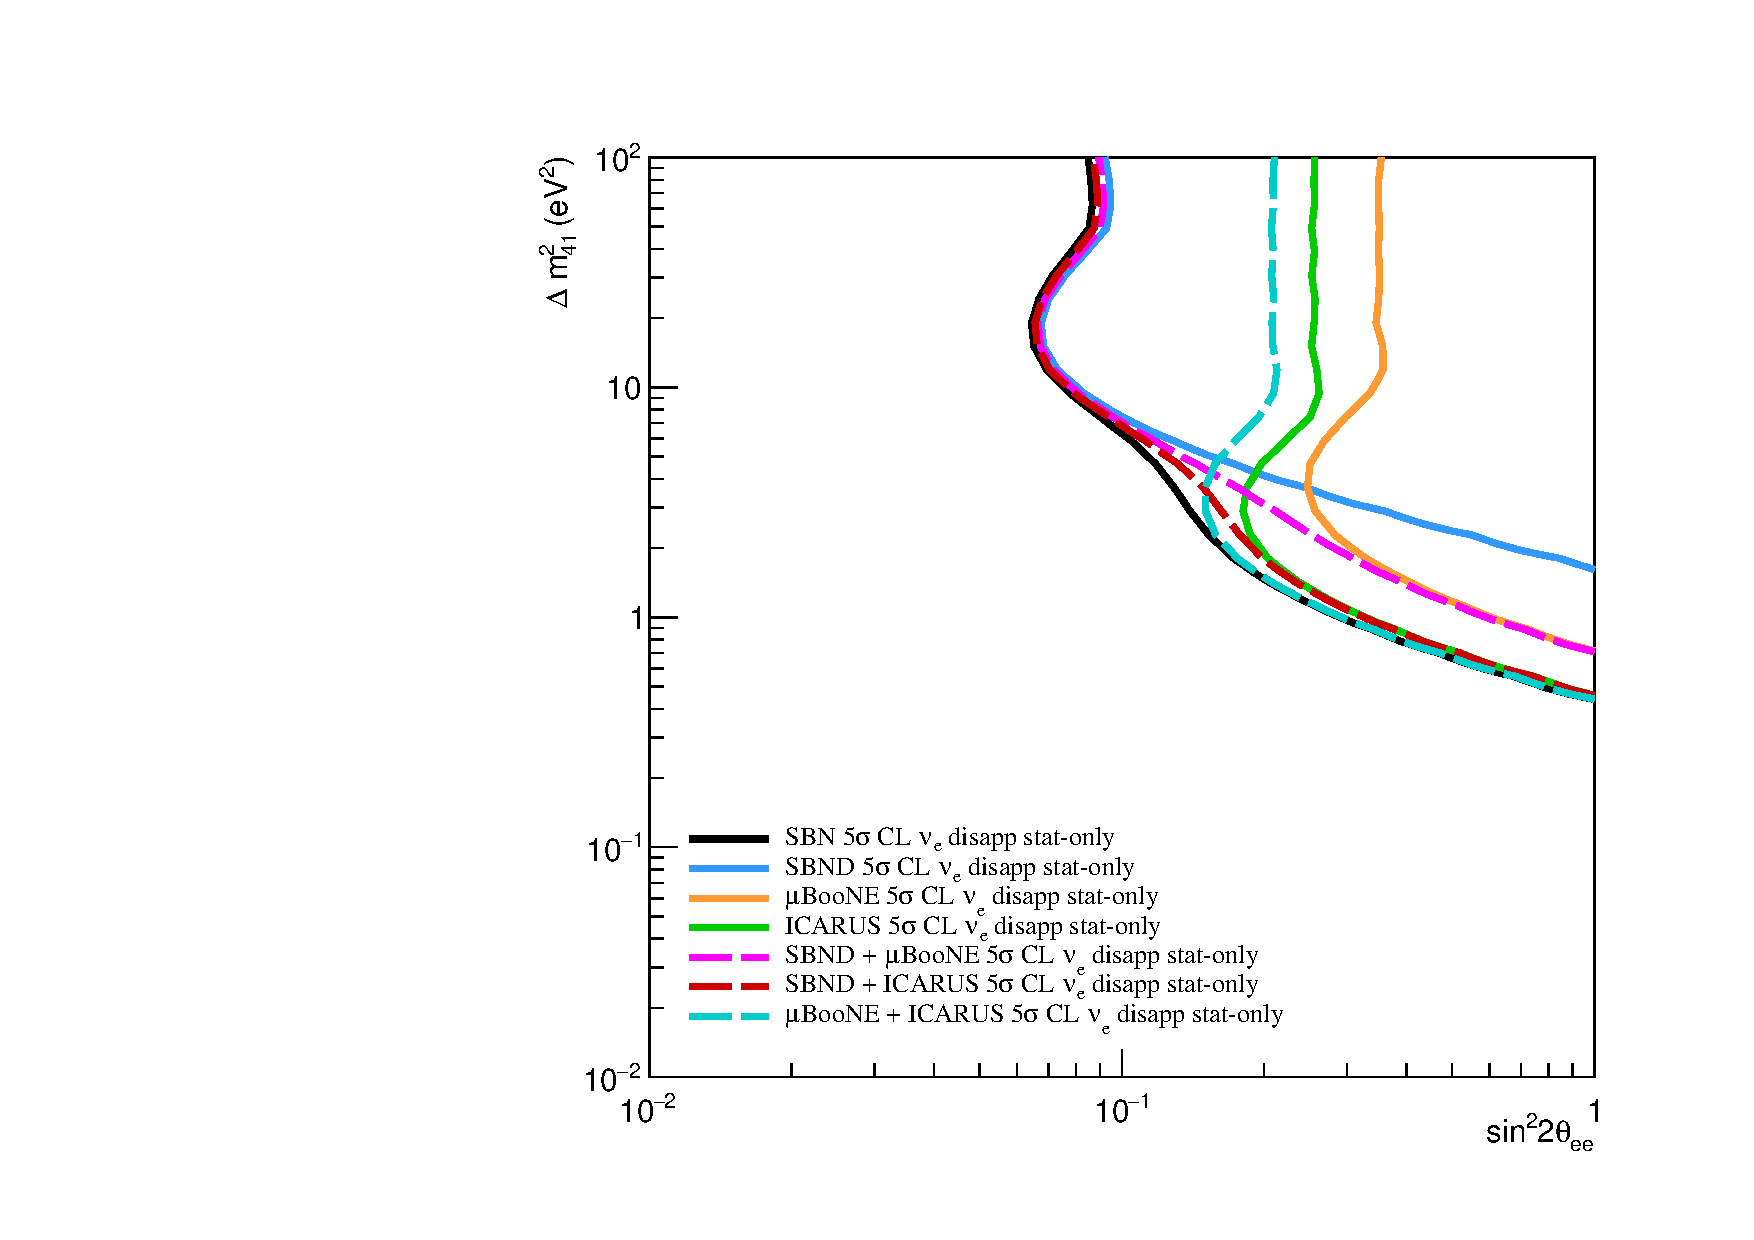
\includegraphics[width = 0.49\textwidth]{figures-chap6/exclusion_contours/nue_disapp_detector_combinations_stat-only.pdf}
    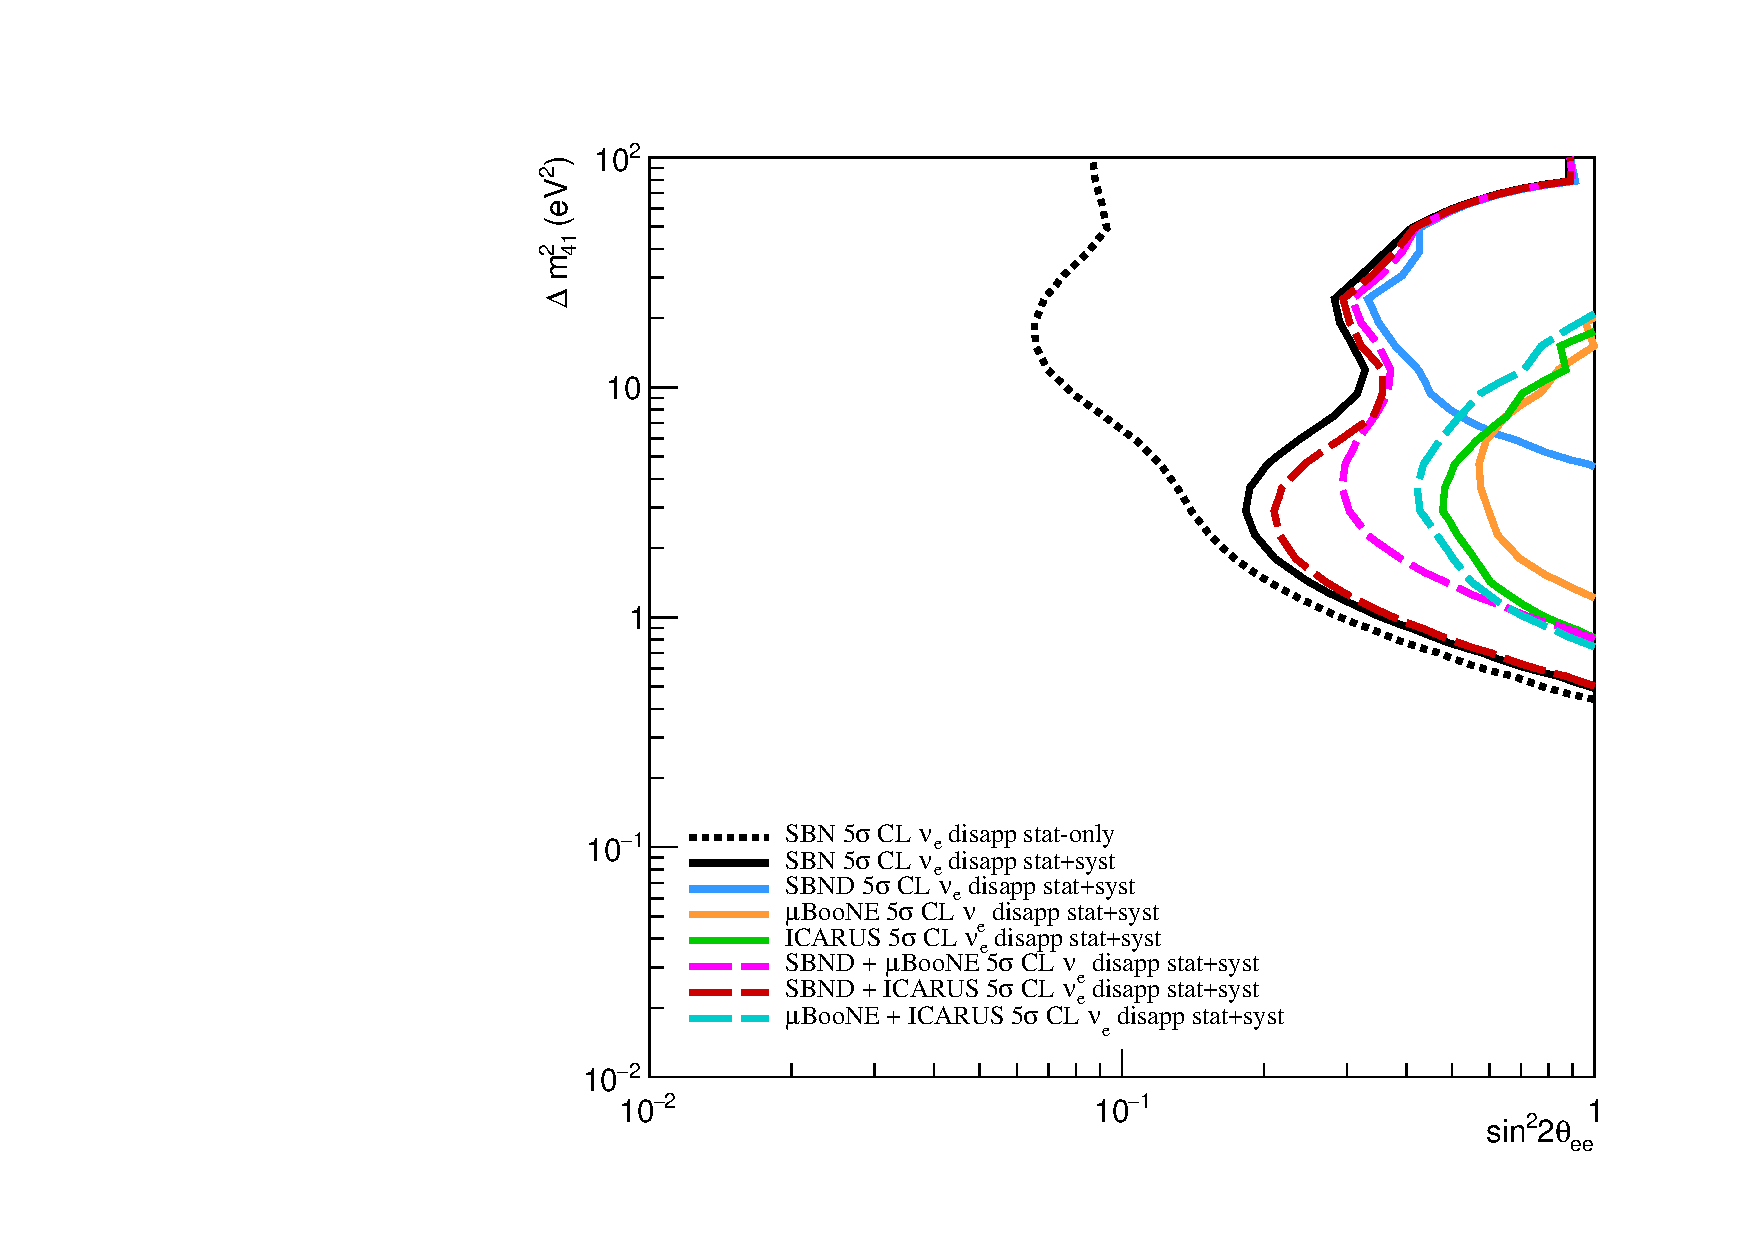
\includegraphics[width = 0.49\textwidth]{figures-chap6/exclusion_contours/nue_disapp_detector_combinations_stat+syst.pdf}
    \caption[\nue disappearance sensitivities from different detector combinations.]{Contributions to the SBN \nue disappearance sterile oscillation sensitivity from each detector and combinations of detectors in the SBN program produced. The statistical-only plots in the left-hand figure show that SBND is most sensitive to the region $\Delta m_{41}^{2} > 3$~eV$^{2}$ and ICARUS is most sensitive below $\Delta m_{41}^{2} < 3$~eV$^{2}$. The right-hand figure includes flux and interaction systematic parameters and highlights the considerable improvement in the oscillation sensitivity when including multiple detectors in the fits.}
    \label{fig:nue_disapp_sensitivity_detector_contribution}
\end{figure}

The relative contribution of the different systematic groups to the overall exclusion contour for \nue disappearance is comparable to the \nue appearance case. The interaction systematics again have the largest impact the majority of which is due to the modern set of parameters. The proposal set of parameters have the smallest impact with the magnitude of the impact from the flux parameters being somewhere in between the two sets of interaction parameters.

\begin{figure}[h!]
    \centering
    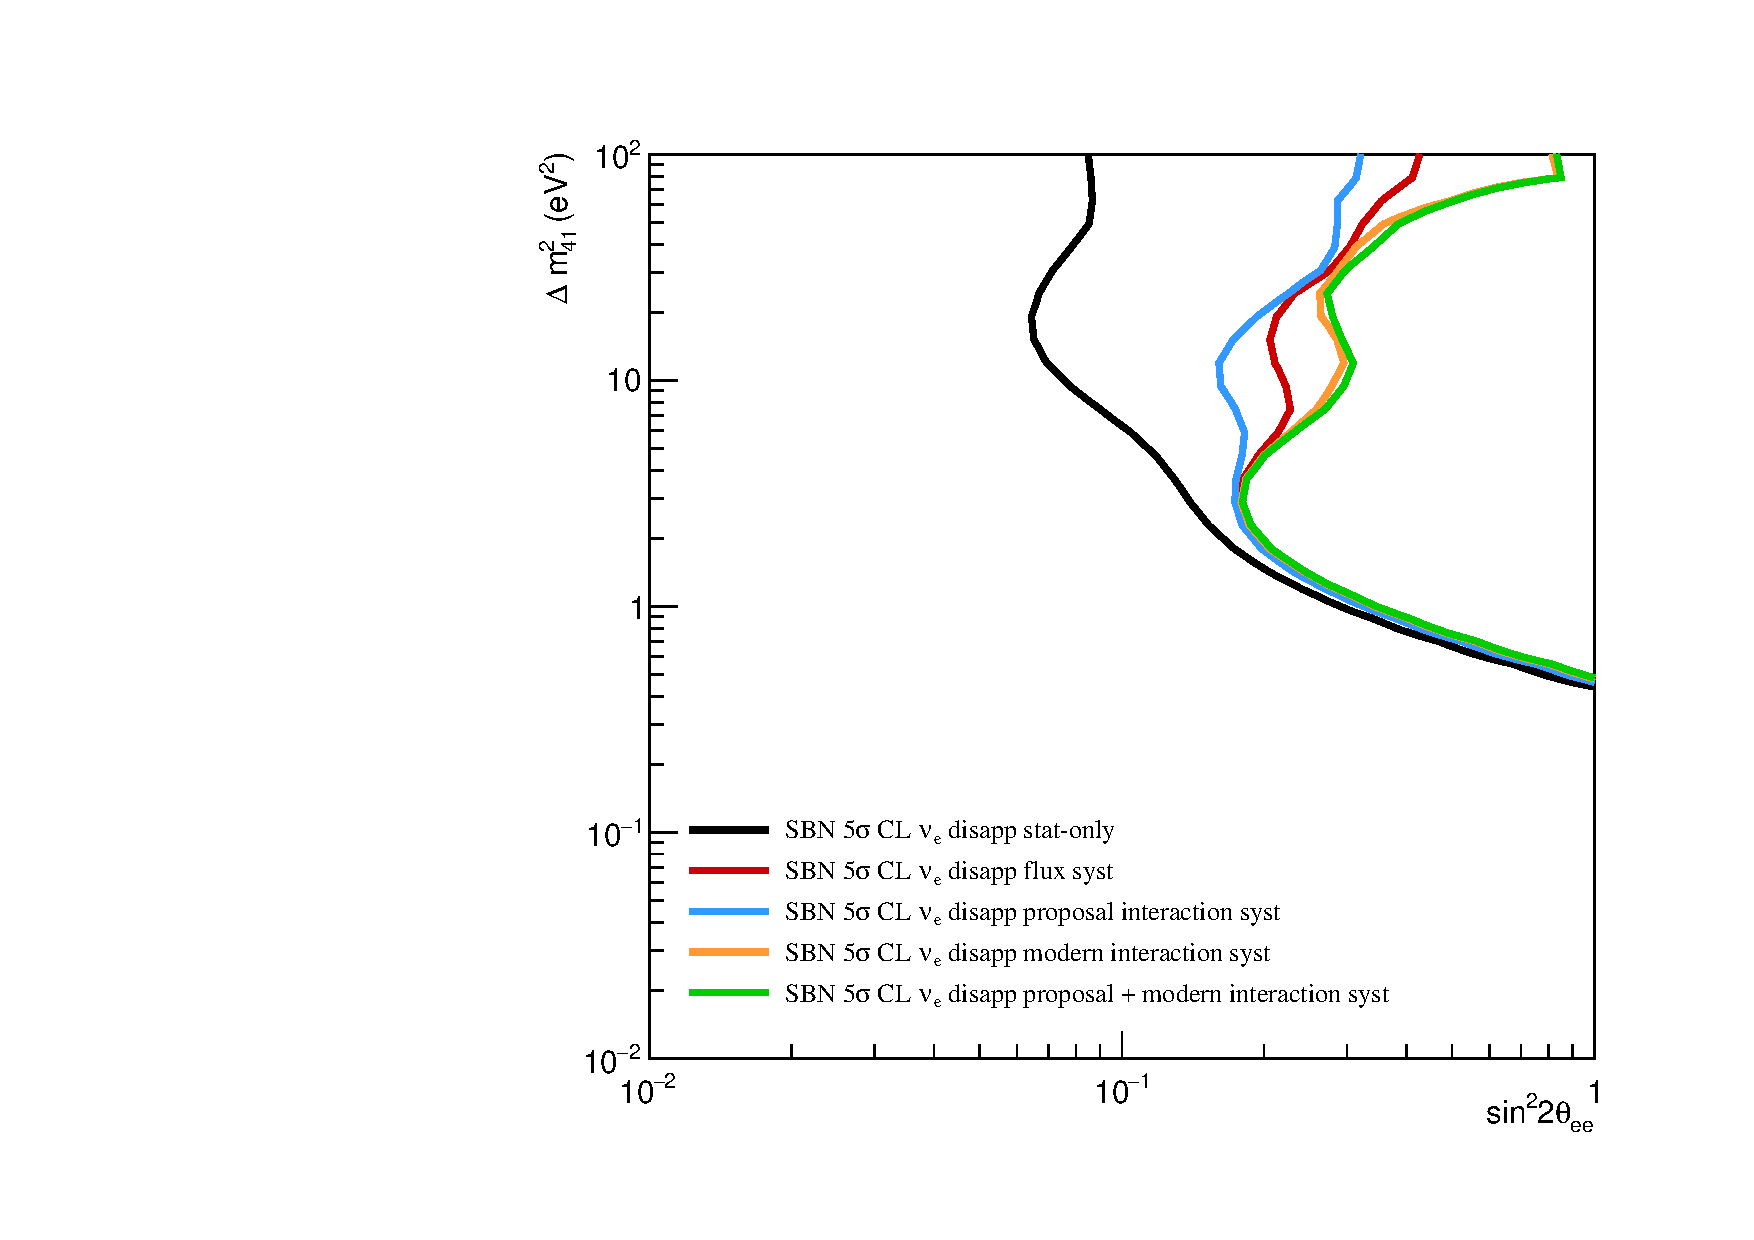
\includegraphics[width = 0.49\textwidth]{figures-chap6/exclusion_contours/nue_disapp_syst_groups.pdf}
    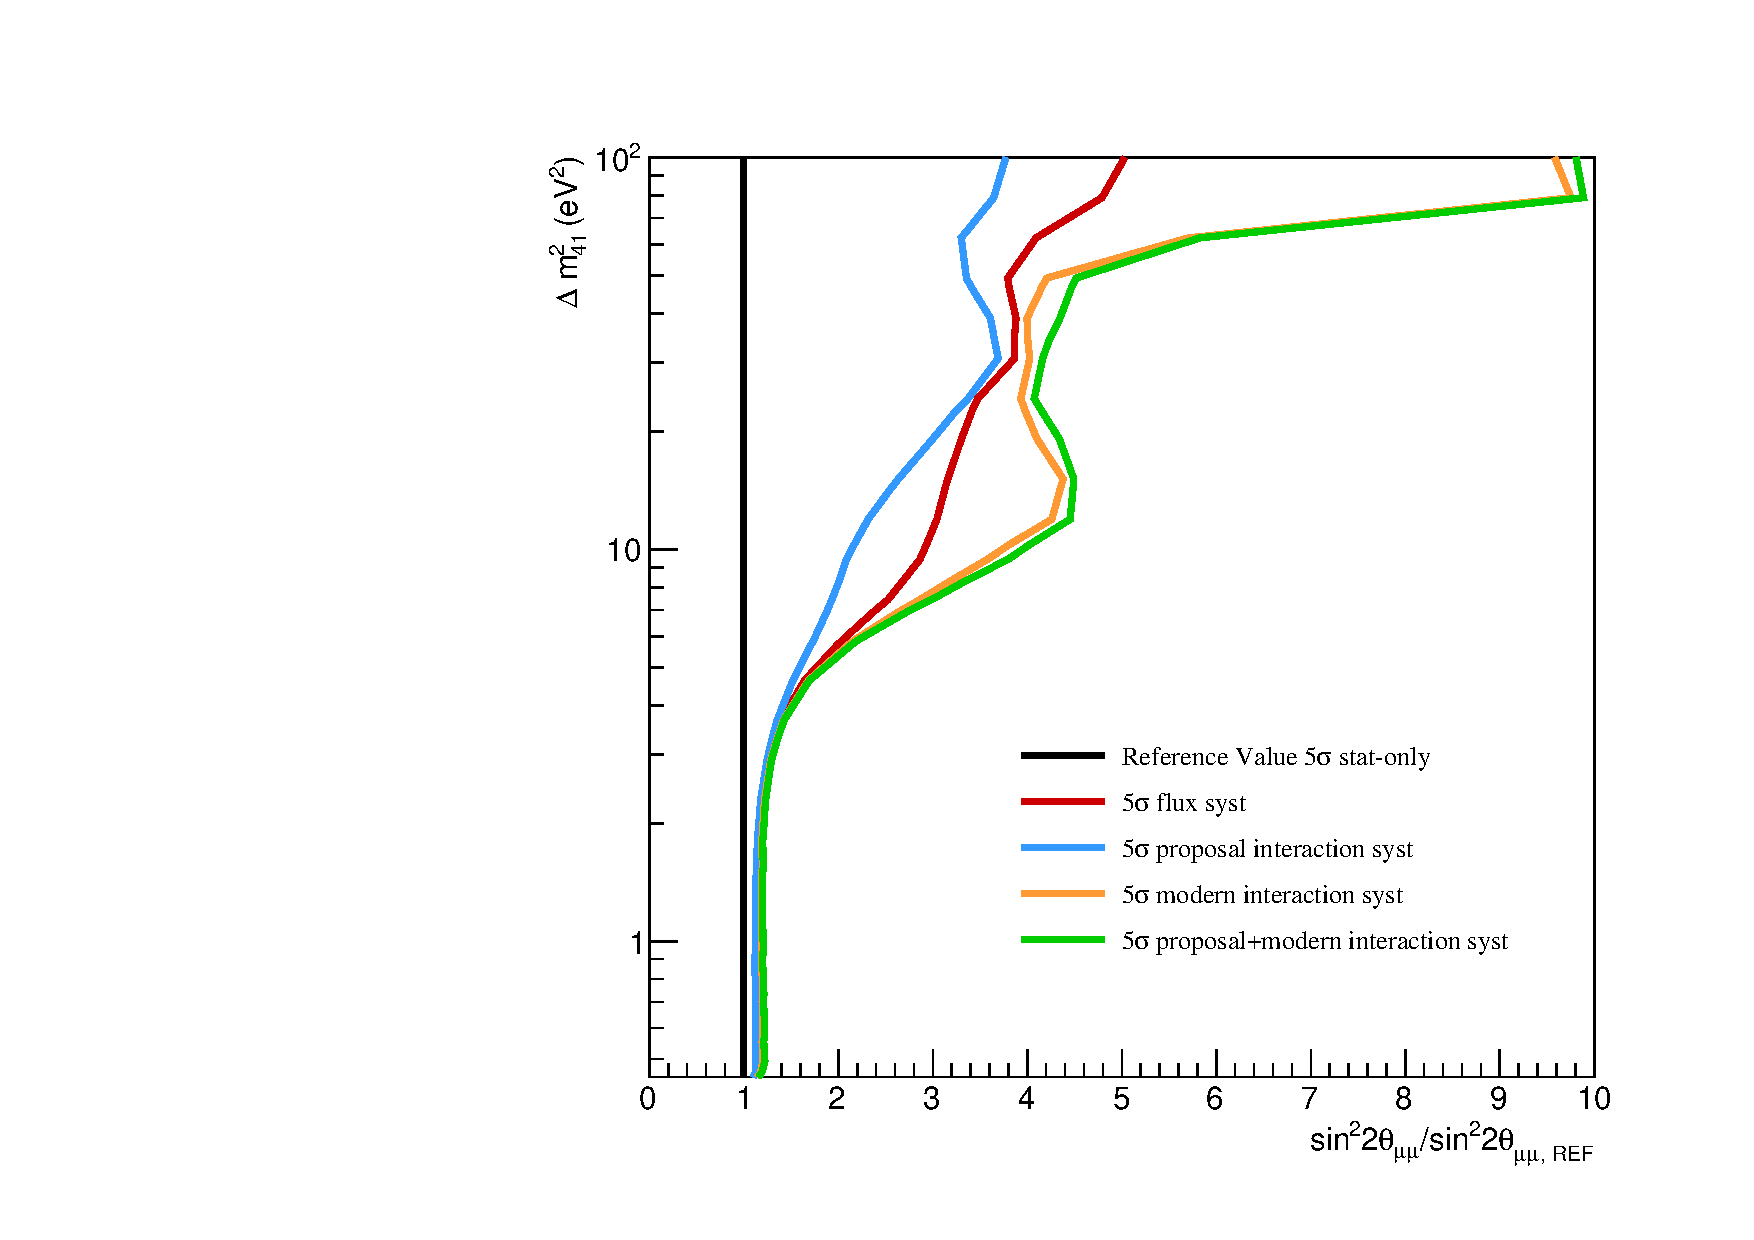
\includegraphics[width = 0.49\textwidth]{figures-chap6/exclusion_contours/nue_disapp_syst_groups_ratios.pdf}
    \caption[\nue app sensitivity reduction from different systematic groups.]{The left plot shows the reduction in sensitivity from the stat-only contour when including each set of systematic parameters in the fits. The right plot shows the relative location of each systematic contour in $\sin^{2}2\theta_{ee}$ space, with respect to the statistical-only case for the active region of $\Delta m_{41}^{2}$ phase space.}
    \label{fig:nue_disapp_syst_groups}
\end{figure}

\newpage
The complete \nue disappearance exclusion sensitivities and allowed regions for both the statistical only case and with the inclusion of flux and interaction systematics are shown in \FigureRef{fig:nue_disapp_global_sensitivity} for the entire \gls{sbn} program alongside external limits from the ND280 detector which serves as one of the near detectors as part of the \gls{t2k} experiment \cite{t2k_experiment}. The results for the \gls{sbn} program are shown at a 5$\sigma$ confidence level whereas the allowed region from the \gls{t2k} experiment is shown at both 68\% and 90\% confidence level and the exclusion contour is at a 95\% confidence level \cite{T2K_nue_disapp_contour}. The results from \gls{sbn} exclude a substantial portion of the \gls{t2k} allowed region with the exclusion limits at high $\Delta m^2_{41}$ not being as strong for the current comparison. 

\begin{figure}
    \centering
    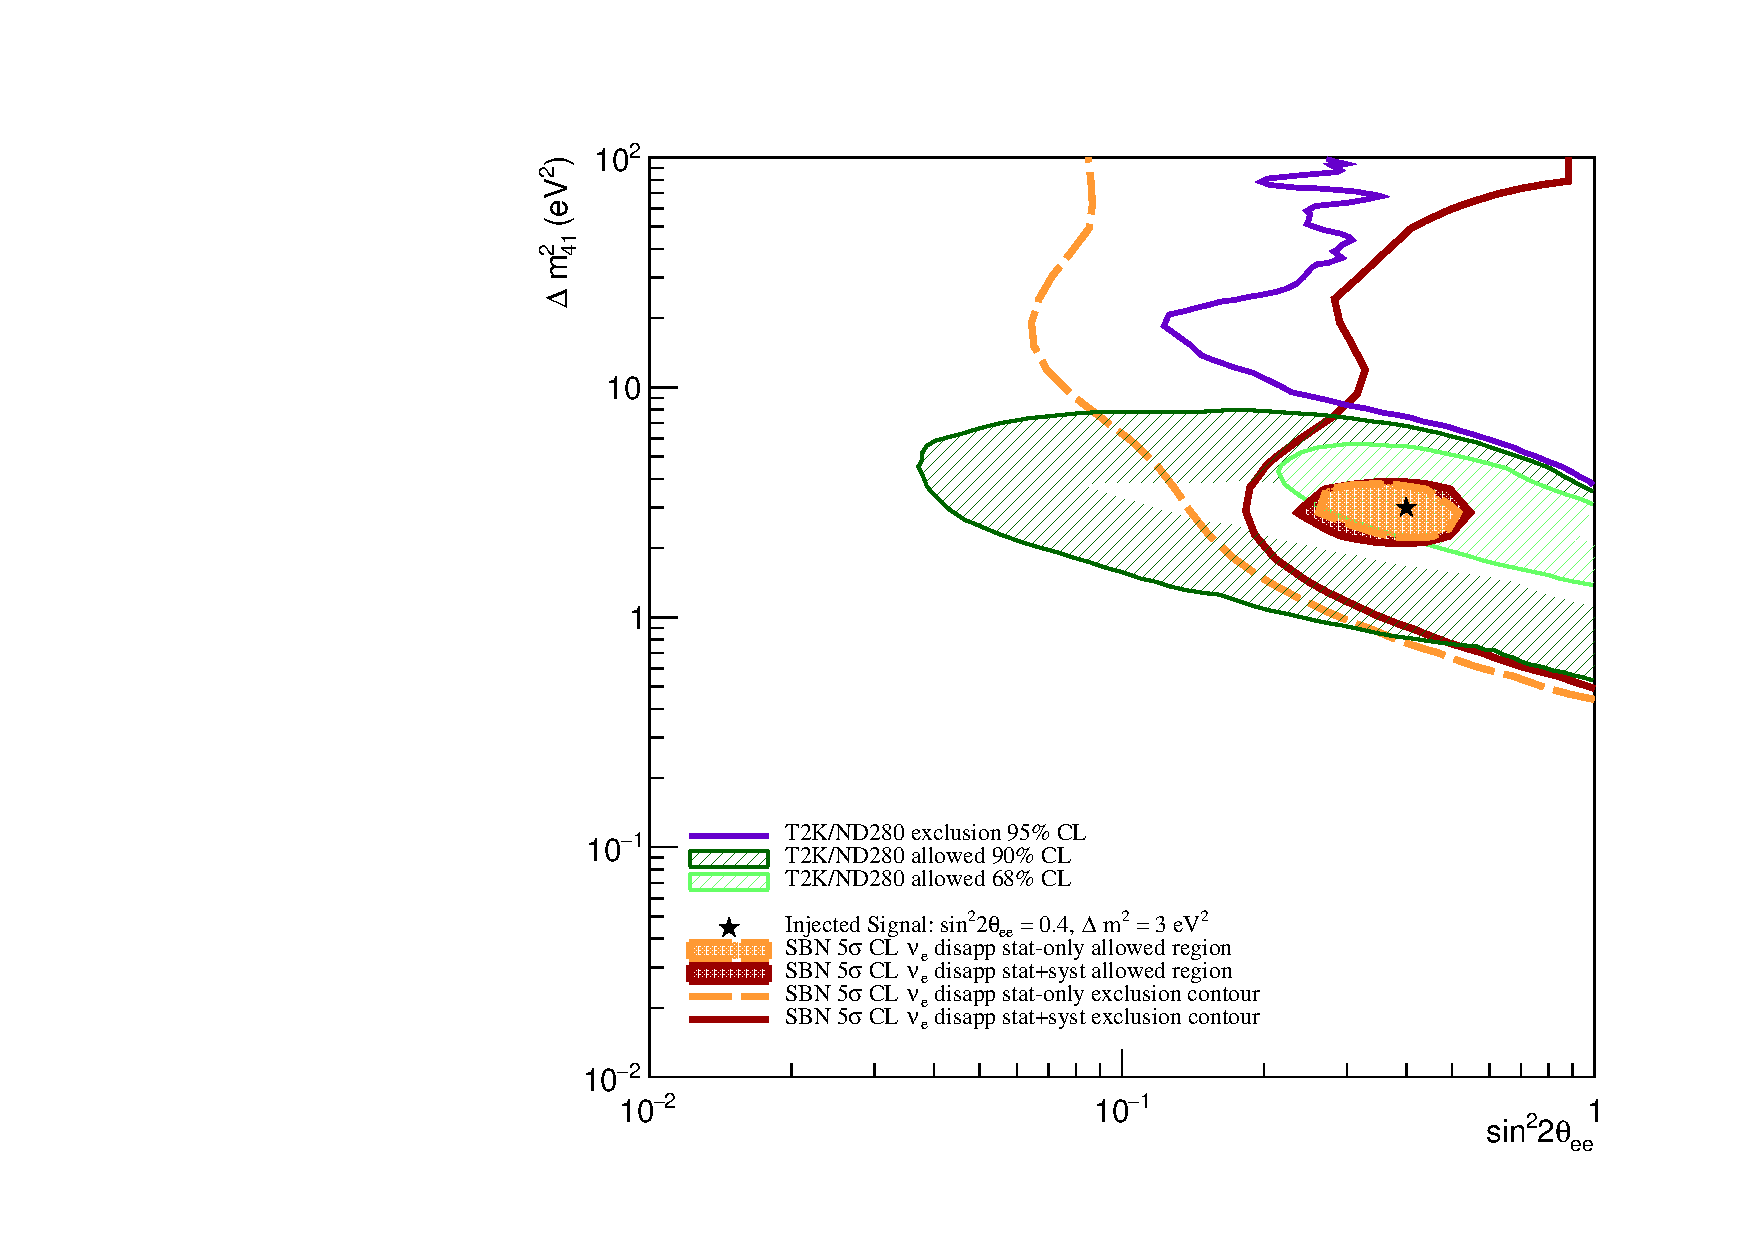
\includegraphics[width = \largefigwidth]{figures-chap6/overlays/valor_overlays_nue_disapp.pdf}
    \caption[\nue disappearance contours with external limits.]{\nue disappearance exclusion contours and allowed regions for the stat only case and with flux and interaction systematic uncertainties included. External limits from the \gls{t2k} experiments have been overlayed \cite{T2K_nue_disapp_contour}. (The confidence intervals for each contour are shown in the legend and it should be noted that those from external limits are not the same as those from the contours produced for the \gls{sbn} program.)}
    \label{fig:nue_disapp_global_sensitivity}
\end{figure}

\newpage
\subsection{\texorpdfstring{\nue Sensitivities Based on Shower Energy Reconstruction}{nue Sensitivities Based on Shower Energy Reconstruction}}

The reconstructed neutrino energy used in the analyses shown so far is based on truth information where smearing has been applied to emulate a reconstructed value. 

To better motivate the reconstructed energy used, the results from \ChapterRef{chap:Energy_Reco} have been used to tweak the true energy of the showering particles (electrons or photons) to emulate a reconstructed energy based on the reconstruction performance that has been observed with the currently available tools. Since only the reconstructed shower energy was actively investigated here, any non-showering particles continue to have their reconstructed energy estimated by directly smearing the true energy. 

The two cases considered for estimating the reconstructed energy of the showering particle are,
\begin{itemize}
    \item A flat negative bias of 20\% is applied to the true energy for all particles.
    \item A flat negative bias applied to the true energy along with an additional variation to emulate the resolution of the reconstruction performance. The magnitude of the bias and the width of the resolution are functions of the true energy. The resolution was emulated by randomly choosing a number based on a Gaussian with a given standard deviation. The three categories used depending on the true energy are shown in \TableRef{table:variable_bias}.

    \begin{table}[h!]
    \begin{tabular}{ccc}
    E [MeV] & Bias & \sigma \\ \hline
    E $<$ 100 & 40\% & 0.15 \\
    100 $\leq$ E $<$ 200 & 30\% & 0.125 \\
    E $>$ 200 & 20\% & 0.1
    \end{tabular}
    \caption[The variable bias and resolution used to emulate reconstructed energy.]{The variable bias and resolution used to emulate reconstructed energy.}
    \label{table:variable_bias}
    \end{table}

\end{itemize}
The simplistic approach of applying a flat 20\% bias was motivated by the conservative results from \FigureRef{fig:fractional_energy_resolution} which shows that the typical bias is of order 20\%. The more involved process of applying an energy dependent bias and resolution are motivated by \FigureRef{fig:reconstruction_as_a_function_of_energy_profile}. It can be seen that above energies of $\sim 200$ MeV, the bias and standard deviation remain fairly constant, but at energies below this, the bias and resolution increase as the energy decreases. 

The full \nue event selection as described in \SectionRef{sec:nue_selection} was repeated but with the above changes applied. The events from these selections were then used to produce exclusion contours using the same systematic uncertainties as previously described. The overall event rate from the selections using the reconstructed information motivated by \ChapterRef{chap:Energy_Reco} is lower than than the traditional method which relied on energy smearing. 

The exclusion contours comparing the three selections are shown on the left of \FigureRef{fig:nue_app_bias} and \FigureRef{fig:nue_disapp_bias} for \nue appearance and disappearance respectively. The difference between the three exclusion contours is relatively minor and therefore the ratios of the contours to the contour from the original selection are shown on the right of their respective figures. Since the event rate is reduced in the updated selections, it is expected that the overall exclusion sensitivity would also be reduced. This indeed the case for most values of $\Delta m^2_{41}$ with only a couple of areas where the selection with the flat 20\% bias appears to improve the sensitivity.

\begin{figure}[h!]
    \centering
    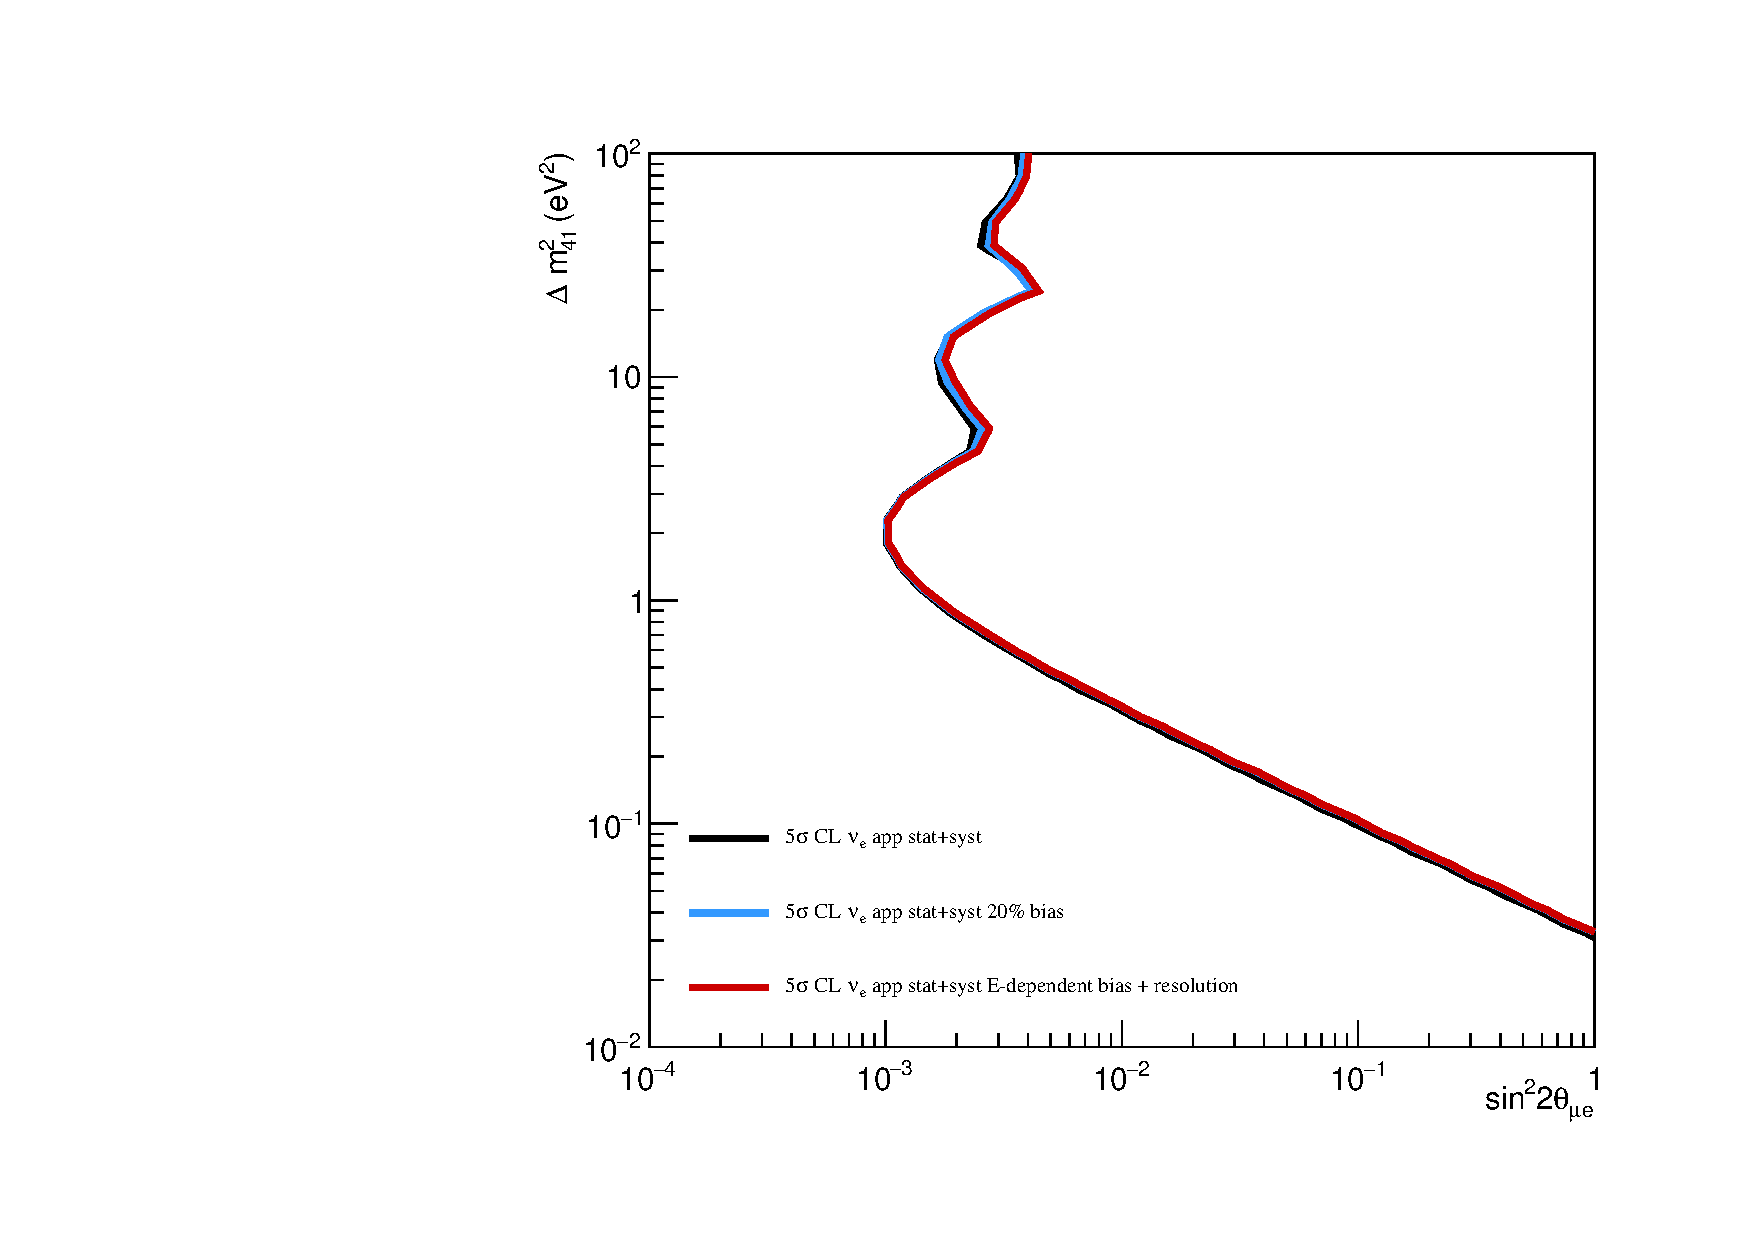
\includegraphics[width = 0.49\textwidth]{figures-chap6/exclusion_contours/bias/nue_app_03d1.pdf}
    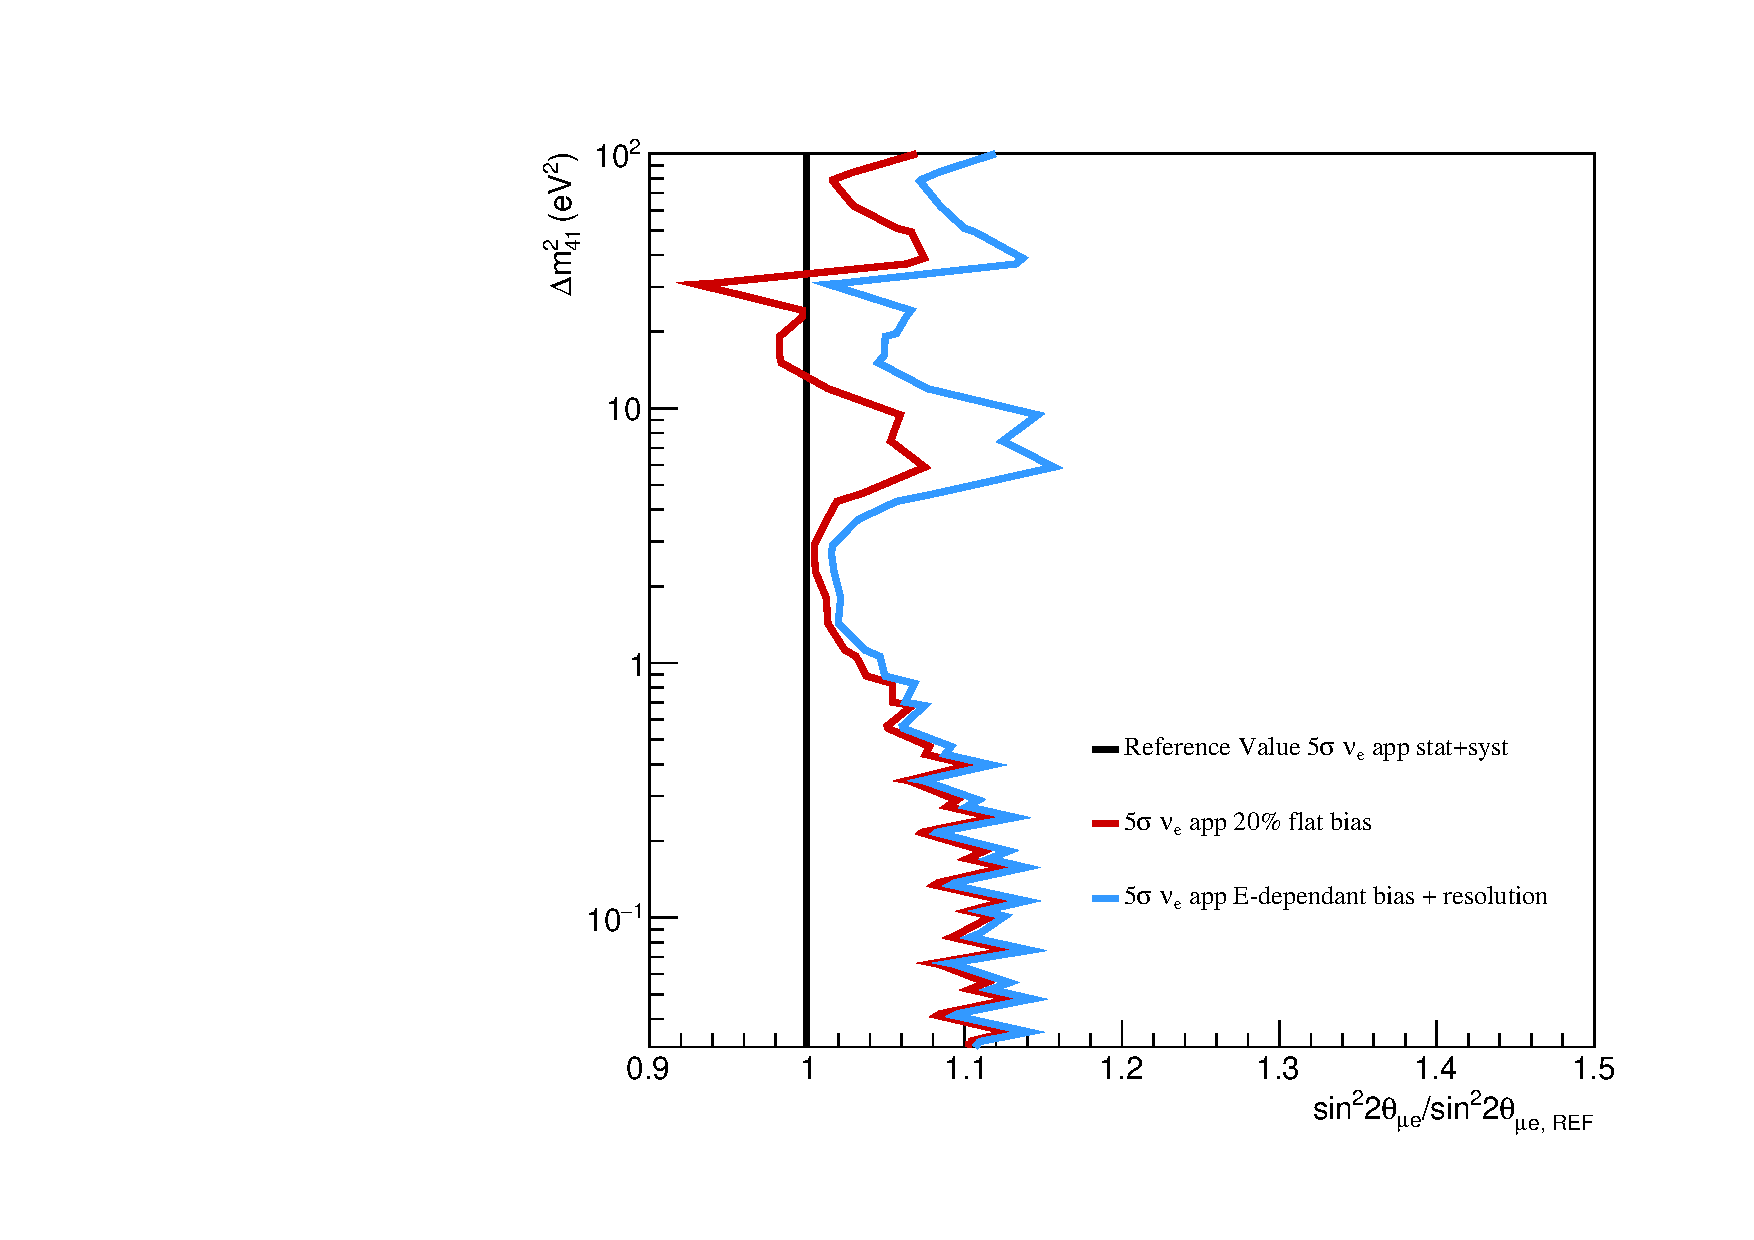
\includegraphics[width = 0.49\textwidth]{figures-chap6/exclusion_contours/bias/nue_app_03d1_ratio.pdf}
    \caption[\nue appearance exclusion contours using events from the selection motivated by \gls{em} shower reconstruction.]{Left: \nue appearance exclusion contours with flux and interaction uncertainties using events from the original selection and the ones motivated by results from \gls{em} shower reconstruction. Right: The ratio of the exclusion contours to the contour from the original selection.}
    \label{fig:nue_app_bias}
\end{figure}

\begin{figure}[h!]
    \centering
    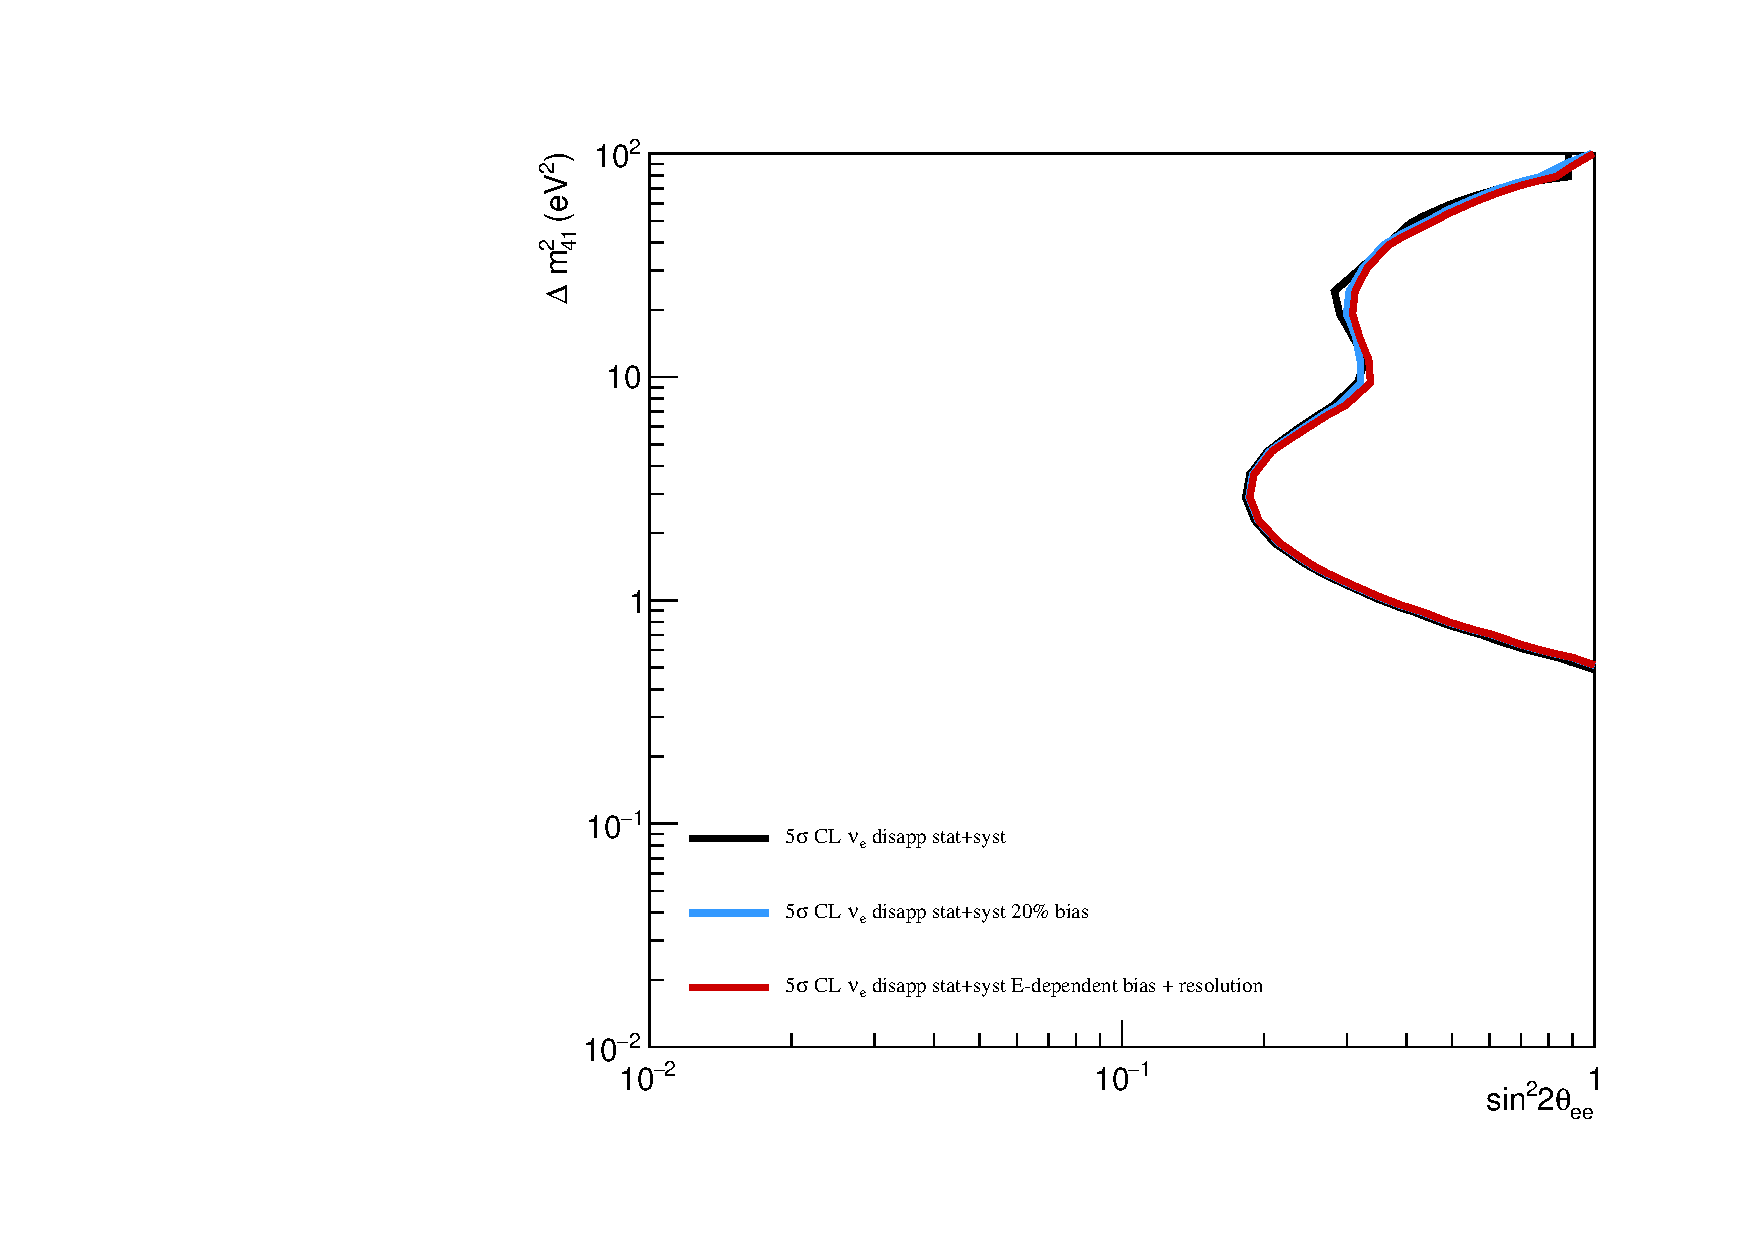
\includegraphics[width = 0.49\textwidth]{figures-chap6/exclusion_contours/bias/nue_disapp_03d1.pdf}
    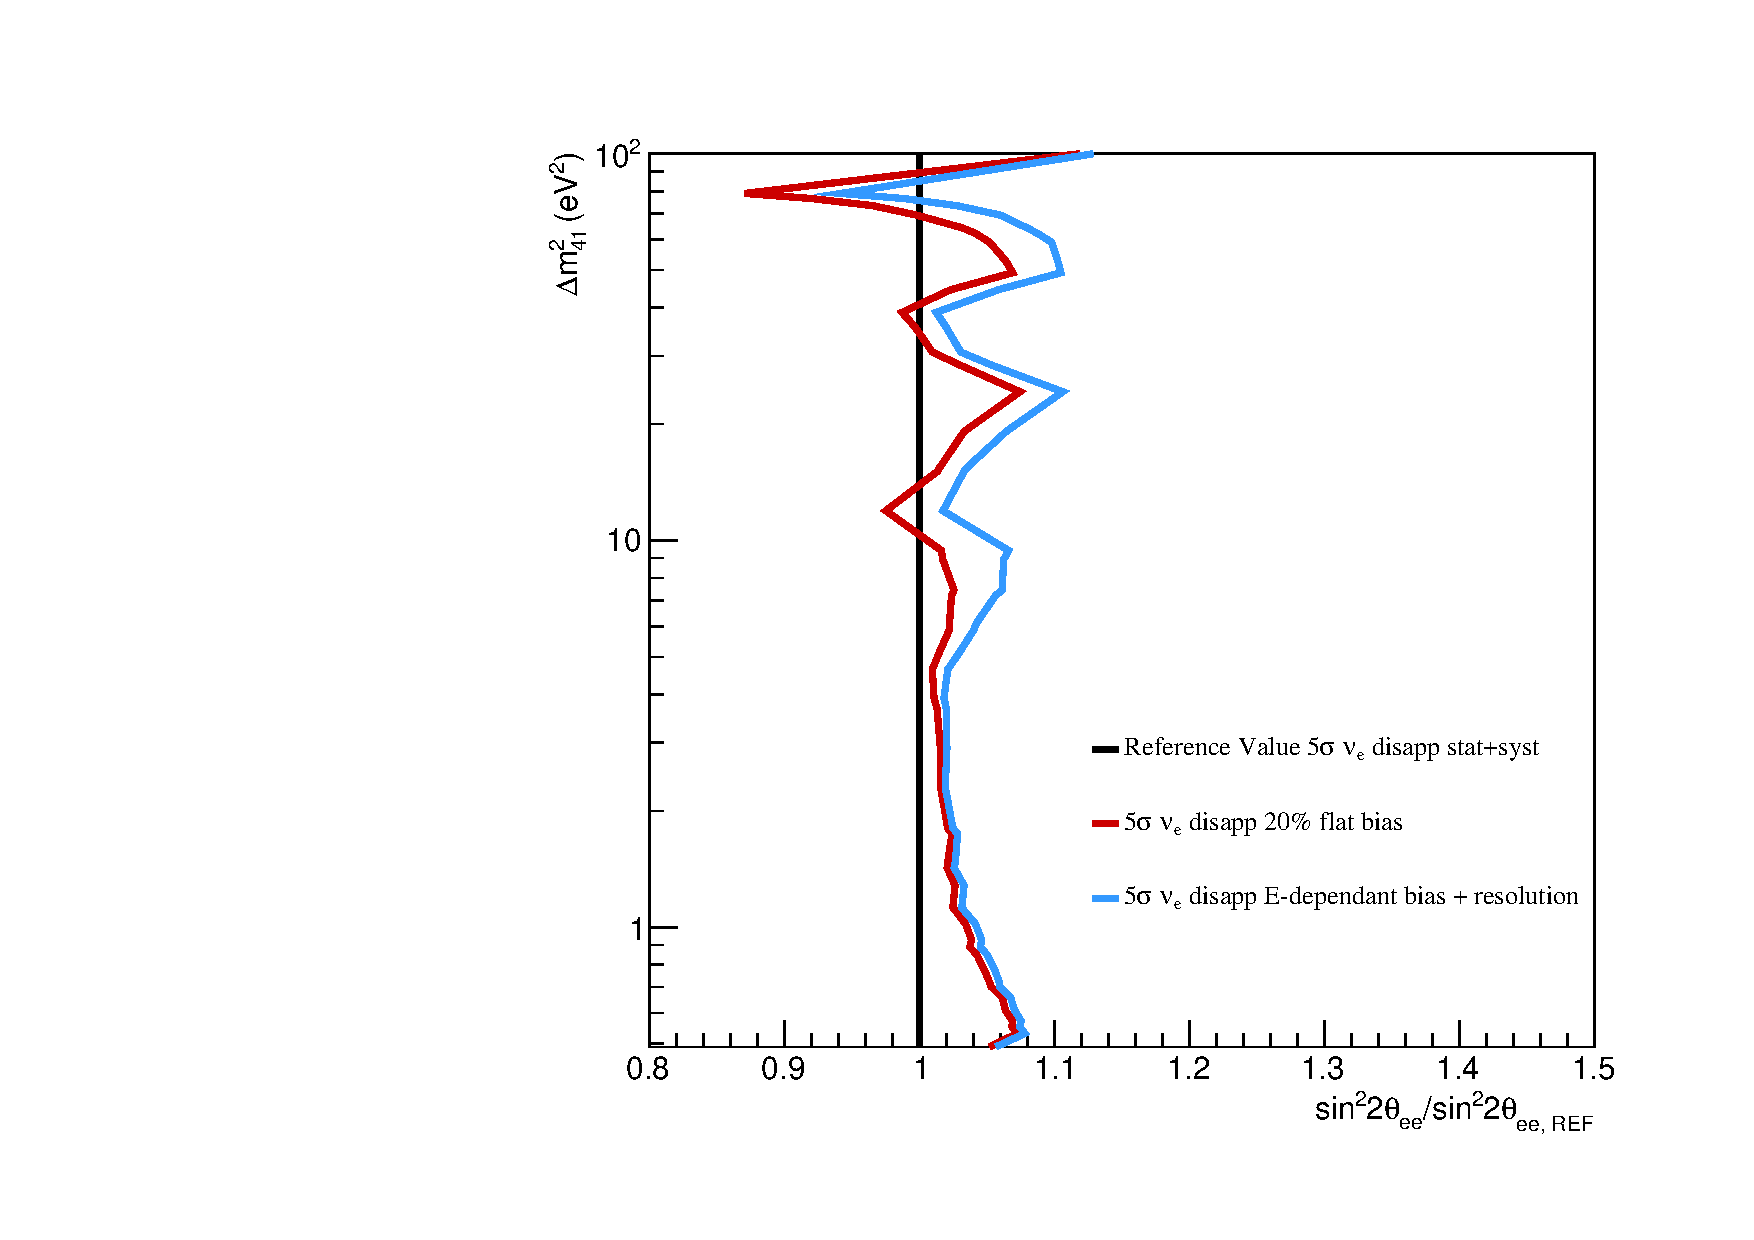
\includegraphics[width = 0.49\textwidth]{figures-chap6/exclusion_contours/bias/nue_disapp_03d1_ratio.pdf}
    \caption[\nue disappearance exclusion contours using events from the selection motivated by \gls{em} shower reconstruction.]{Left: \nue disappearance exclusion contours with flux and interaction uncertainties using events from the original selection and the ones motivated by results from \gls{em} shower reconstruction. Right: The ratio of the exclusion contours to the contour from the original selection.}
    \label{fig:nue_disapp_bias}
\end{figure}

\newpage
\section{\texorpdfstring{\numu Disappearance Analysis}{numu Disappearance Analysis}}

A similar analysis and validation to that described in  \SectionRef{sec:systematic_validation} and \SectionRef{sec:nue_analysis} that was performed for the two \nue channels was also done for the \numu disappearance channel.

The nominal event rate breakdown for each of the detectors is shown in \FigureRef{fig:numu_disapp_spectra} where an integrated spectrum with oscillation parameters $\sin^2{2\theta_{\mu \mu}} = 0.072$, $\Delta m^2_{41} = 1.32 \text{ eV}^2$ has been overlayed. The overall magnitude of the event rate is several order of magnitude greater than that for \nue owing to the fact that the \gls{bnb} consists predominantly of \numu. As was the case for \nue disappearance, the reduction in events for \gls{sbnd} is relatively small whereas for \gls{microboone} and \gls{icarus} it is much more significant.

The complete \numu disappearance exclusion sensitivities and allowed regions for both the statistical only case and with the inclusion of flux and interaction systematics are shown in \FigureRef{fig:numu_disapp_global_sensitivity} for the entire \gls{sbn} program alongside external limits from \gls{minos} and its successor \gls{minos}+, combined results from \gls{sciboone} and \gls{miniboone} and the IceCube experiment \cite{MINOS+} \cite{MiniBooNE/SciBooNE_numu_disapp_contour} \cite{IceCube_numu_disapp_contour}. The results for the \gls{sbn} program are shown at a 5$\sigma$ confidence level whereas the exclusion region from the \gls{minos}/\gls{minos}+, \gls{sciboone}/\gls{miniboone} and IceCube experiments are shown at the 90\% confidence. The IceCube experiment also shows an allowed region at the 99\% confidence level. The results from \gls{sbn} show a stronger sensitivity to that obtained be \gls{miniboone}/\gls{sciboone} for all mass splitting values. The exclusion contour is also comparable to that from \gls{minos}/\gls{minos}+ for $\Delta m^2_{41} \gtrsim 1\text{ eV}^2$, however below this value \gls{minos}/\gls{minos}+ provides a stronger limit. The exclusion contour from IceCube again provides a stronger limit at $\Delta m^2_{41} \lesssim 1\text{ eV}^2$, but for higher values, \gls{sbn} expects to improve on the results from IceCube. The allowed region from IceCube intersect the one from \gls{sbn} so they aren't fully compatible. 

\begin{figure}[h!]
  {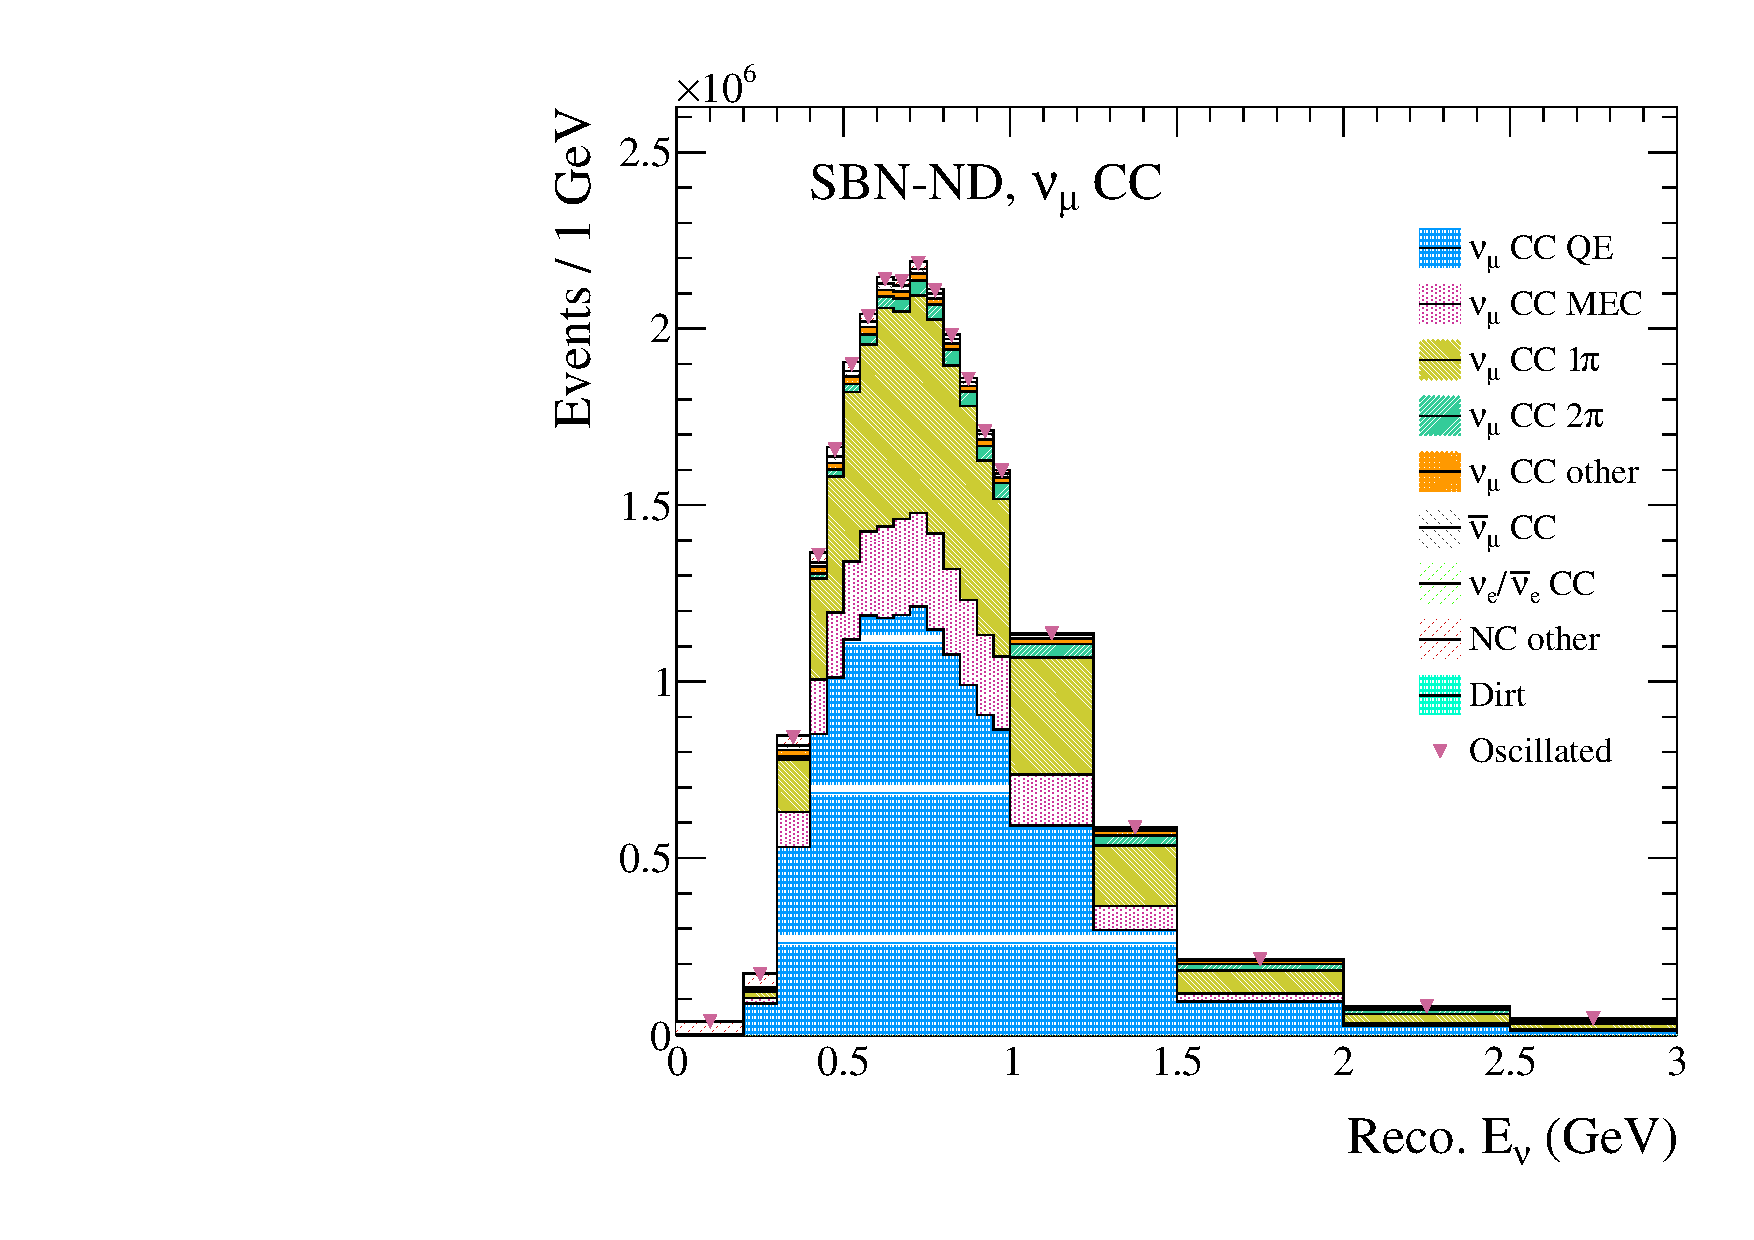
\includegraphics[width=0.49\textwidth]{figures-chap6/spectra/numu_disapp_overlay_dmsq_1.32_sinsq2th_0.072_spectrum_sbn_nd_BNB_FHC_0_modes.pdf}}
  {\includegraphics[width=0.49\textwidth]{figures-chap6/spectra/numu_disapp_overlay_dmsq_1.32_sinsq2th_0.072_spectrum_sbn_uboone_BNB_FHC_1_modes.pdf}}
  {\includegraphics[width=0.49\textwidth]{figures-chap6/spectra/numu_disapp_overlay_dmsq_1.32_sinsq2th_0.072_spectrum_sbn_icarus_BNB_FHC_2_modes.pdf}}
  \captionsetup{width=0.49\textwidth}
  \parbox[b]{0.49\textwidth}%
  {
    \caption[SBN \numu CC inclusive reconstructed neutrino energy spectra with oscillated spectrum overlayed]{The breakdown of the nominal \numu disappearance spectra overlayed with an integrated oscillated spectrum with oscillation parameters, $\sin^2{2\theta_{\mu \mu}} = 0.072$ and $\Delta m^2_{41} = 1.32$~eV$^2$ showing the decrease in event rate.\\\phantom{.}\\\phantom{.}\\\phantom{.}\\}
    \label{fig:numu_disapp_spectra} 
  }
\end{figure}

\begin{figure}[h!]
    \centering
    \includegraphics[width = \largefigwidth]{figures-chap6/overlays/valor_overlays_numu_disapp.pdf}
    \caption[\numu disappearance contours with external limits.]{\numu disappearance exclusion contours and allowed regions for the stat only case and with flux and interaction systematic uncertainties included. External limits from the MINOS/MINOS+, MiniBooNE/SciBooNE and IceCube experiments have been overlayed \cite{MINOS_numu_disapp_contour}\cite{MiniBooNE/SciBooNE_numu_disapp_contour}\cite{IceCube_numu_disapp_contour}. (The confidence intervals for each contour are shown in the legend and it should be noted that those from external limits are not the same as those from the contours produced for the \gls{sbn} program.)}
    \label{fig:numu_disapp_global_sensitivity}
\end{figure}

For a complete discussion of the \numu disappearance channel, see \cite{Rhiannon's_thesis}.

\clearpage

\section{Additional Efficiency and Energy Scale Systematics}

As was mentioned in \SectionRef{sec:other_syst}, efficiency systematics are not currently included in the \textit{standard} analyses. In order to get a measure of the possible impact of efficiency systematics on the sensitivity, various covariance matrices were produced following the scheme outlined in \SectionRef{sec:efficiency_syst}. Matrices were produced to investigate the impact of;
\begin{enumerate}
    \item Fully correlated errors only.
    \item Various combinations of uncorrelated errors with a fixed correlated error.
    \item Uncorrelated errors only applied to a single detector at a time.
    \item A poorly constrained uncorrelated error on a single set of bins.
\end{enumerate}
Unless otherwise stated, the uncertainties from efficiency covariance matrices are applied in addition to the flux and interaction systematics. 

The study of the impact of different efficiency uncertainties was first done for the \numu channel because it was expected that there would be a greater impact than for either of the \nue channels. This is because the typical event rate for the \numu channel is several order of magnitude greater than that of \nue meaning that the \numu channel is systematics limited whereas the \nue channels may tend towards being statistics limited. Once a contour becomes statistics limited, continuing to apply additional systematic uncertainties will begin to have diminishing impacts. 

\subsection{\texorpdfstring{Impact of Efficiency Systematics on \numu Disappearance Sensitivities}{Impact of Efficiency Systematics on numu Disappearance Sensitivities}}


The impact of fully correlated uncertainties up to 10\% are shown on the left of \FigureRef{fig:numu_corr_uncorr_error} whilst keeping the uncorrelated uncertainty at 0\%. The right plot shows the impact of increasing the uncorrelated uncertainties uniformly across all bins with a fixed correlated uncertainty of 2\%. It follows that for even relatively large correlated uncertainties the impact on the sensitivity is minor and that any reduction in sensitivities will be largely dominated by the uncorrelated uncertainty. 

\begin{figure}[!h]
    \centering
    \includegraphics[width = 0.49\textwidth]{figures-chap6/exclusion_contours/efficiency_systematics/numu_disapp_Xpct_cor.pdf}
    \includegraphics[width = 0.49\textwidth]{figures-chap6/exclusion_contours/efficiency_systematics/numu_disapp_2pct_cor_Xpct_uncor.pdf}
    \caption[Impact of correlated and uncorrelated efficiency systematics on the \numu disappearance channel.]{The impact on the \numu disappearance exclusion sensitivity by applying fully correlated uncertainties ranging from 1\% to 10\% to all bins (Left) and by applying a fixed 2\% fully correlated uncertainty with additional uncorrelated uncertainty ranging from 0.5\% to 2\% across all bins (Right). }
    \label{fig:numu_corr_uncorr_error}
\end{figure}

\FigureRef{fig:numu_uncorr_det} shows the impact of applying a 2\% uncorrelated uncertainty only to each of the \gls{sbn} detectors one at a time. The \gls{microboone} detector has a minor impact at around $\Delta m ^2_{41} = 10$ eV$^2$ and close to no impact at small and large $\Delta m ^2_{41}$ values. The \gls{icarus} detector has a larger impact for most $\Delta m ^2_{41}$ values but again only has a minor contribution at very large $\Delta m ^2_{41}$ values. Across most $\Delta m ^2_{41}$ values greater than $\sim$0.5 eV$^2$, \gls{sbnd} dominates the sensitivity. At values below 0.5 eV$^2$ the reduction in sensitivity due to \gls{sbnd} and \gls{icarus} are comparable. This point is emphasised in \FigureRef{fig:numu_uncorr} where the fully correlated uncertainty is fixed at 2\% and the uncorrelated uncertainty is set to 2\% for one of the three \gls{sbn} detectors whilst being set to 0.5\% for the other two detectors. The contour where \glspl{sbnd} uncorrelated uncertainty is set to 2\% looks similar to the corresponding contour in \FigureRef{fig:numu_uncorr_det}. It has been shown that the uncorrelated component of the uncertainty has a large impact when compared to the correlated component and that any efficiency uncertainties impact \gls{sbnd} more than the other two detectors so this result ought to be expected. Similarly, the two contours where uncorrelated uncertainty is set to 2\% for \gls{microboone} and \gls{icarus} are pulled towards the \gls{sbnd} contour since despite it having a smaller associated uncorrelated uncertainty, it will still contribute significantly. 

\begin{figure}[!h]
    \centering
    \includegraphics[width = \largefigwidth]{figures-chap6/exclusion_contours/efficiency_systematics/numu_disapp_2pct_uncor_per_detector.pdf}
    \caption[Impact of a 2\% uncorrelated efficiency systematic on the \numu disappearance channel for each individual detector.]{The impact on the \numu disappearance exclusion sensitivity by applying a 2\% uncorrelated efficiency uncertainty to a single one of the three \gls{sbn} detectors.}
    \label{fig:numu_uncorr_det}
\end{figure}

\begin{figure}[!h]
    \centering
    \includegraphics[width = \largefigwidth]{figures-chap6/exclusion_contours/efficiency_systematics/numu_disapp_2pct_cor_2pct_X_05pct_other_per_detector_uncor.pdf}
    \caption[Impact of a 2\% uncorrelated efficiency systematic for one detector and 0.5\% for the other two on the \numu disappearance channel.]{The impact on the \numu disappearance exclusion sensitivity by applying a 2\% fully correlated efficiency uncertainty for each of the \gls{sbn} detectors and a 2\% uncorrelated uncertainty for one of detectors and a 0.5\% uncorrelated uncertainty for the other two detectors. This is repeated for each of the detectors. The associated covariance matrix used for the case where \glspl{sbnd} uncorrelated uncertainty was set to 2\% is shown in the bottom left plot of \FigureRef{fig:efficiency_cov_matrices}.}
    \label{fig:numu_uncorr}
\end{figure}

\newpage
Instead of exploring the impact from fully uncorrelated uncertainties or a constant uncorrelated uncertainty across all bins in a detector, \FigureRef{fig:numu_bulk_uncorr} considers the case where a single set of bins are poorly constrained. The sets of bins considered are,
\begin{itemize}
    \item CC signal below the peak energy ($< 0.6$ GeV),
    \item CC signal at the peak energy ([0.6 - 1.0] GeV),
    \item CC signal above the peak energy ($> 1.0$ GeV),
    \item Background.
\end{itemize}
In each case, the uncorrelated uncertainty for the bins of interest are set to 2\% in each of the \gls{sbn} detectors, whilst the rest of the uncorrelated uncertainties are set to 0.5\% and the fully correlated uncertainty is fixed at 2\%. Increasing the uncertainty associated with the background bins has the smallest impact whereas increasing the uncertainty for the high and low energy bins has the largest impact at large and small $\Delta m^2_{41}$ respectively. The peak energy bins also contribute significantly around $\Delta m^2_{41}$ equal to 1 eV$^2$ and 10 eV$^2$. 


\begin{figure}[!h]
    \centering
    \includegraphics[width = \largefigwidth]{figures-chap6/exclusion_contours/efficiency_systematics/numu_disapp_2pct_cor_05pct_bulk_2pct_X_uncor.pdf}
    \caption[\numu disapp with poorly constrained efficiency systematic for a set of bins.]{The impact on the \numu disappearance exclusion sensitivity by applying a 2\% fully correlated efficiency uncertainty for each of the \gls{sbn} detectors and a 0.5\% uncorrelated uncertainty for all but a single set of bins where the uncorrelated uncertainty is set to 2\%. The 'peak' energy bins are defined as those covering an energy range of [0.6,~1.0] GeV. The 'high' and 'low' energy bins are defined as those covering energies above and below the peak energy respectively and the 'bkg' bins are all the bins associated with background events. The set of bins of interest are applied to each of the three detectors and the covariance matrix for where the peak energy bins are the ones in question is shown in the bottom right plot of \FigureRef{fig:efficiency_cov_matrices}.}
    \label{fig:numu_bulk_uncorr}
\end{figure}


\clearpage
\subsection{\texorpdfstring{Impact of Efficiency Systematics on \nue Appearance Sensitivities}{Impact of Efficiency Systematics on nue Appearance Sensitivities}}

In order to gauge the contribution of some typical efficiency uncertainty, \FigureRef{fig:nue_app_syst_groups+efficiency} shows the impact on the \nue appearance sensitivity from individual sets of systematic parameters as in \FigureRef{fig:nue_app_syst_group_sensitivities} but with the addition of a 2\% correlated + 2\% uncorrelated efficiency uncertainty. The impact of the efficiency uncertainty is comparable to the proposal interaction systematics having the smallest contribution to the sensitivity. 

\begin{figure}[h!]
    \centering
    \includegraphics[width = \largefigwidth]{figures-chap6/exclusion_contours/nue_app_syst_groups+det.pdf}
    \caption[\nue app sensitivity reduction from different systematic groups with a (2+2)\% efficiency uncertainty.]{The reduction in the \nue appearance sensitivity from the stat-only contour when including each set of systematic parameters in the fits. Similar to \FigureRef{fig:nue_app_syst_group_sensitivities} but with the addition of a 2\% correlated and 2\% uncorrelated efficiency uncertainty.}
    \label{fig:nue_app_syst_groups+efficiency}
\end{figure}

The reduction in sensitivity from applying a 10\% correlated uncertainty and a 2\% correlated + 2\% uncorrelated uncertainty are shown in \FigureRef{fig:nue_app_corr_uncorr_error}. Since a correlated error of 10\% has a close to negligible impact, the results from applying correlated uncertainties less than 10\% as was done for the \numu channel have been omitted. Similarly, applying smaller uncorrelated uncertainties would again only have a minor impact so these have also been omitted.  

\begin{figure}[h!]
    \centering
    \includegraphics[width = \largefigwidth]{figures-chap6/exclusion_contours/efficiency_systematics/nue_app_cor_uncor.pdf}
    \caption[Impact of correlated and uncorrelated efficiency systematics on the \nue appearance sensitivity.]{The impact on the \nue appearance exclusion sensitivity by applying a 10\% fully correlated efficiency uncertainty to all bins and by applying 2\% fully correlated + 2\% uncorrelated efficiency uncertainty.}
    \label{fig:nue_app_corr_uncorr_error}
\end{figure}

\FigureRef{fig:nue_app_uncorrelated_per_detector} asses the impact of a 2\% uncorrelated uncertainty which is applied to each detector one at a time. Applying the uncertainty to \gls{microboone} and \gls{icarus} appears to have a negligible impact across all $\Delta m^2_{41}$ values. \gls{sbnd} has a relatively small impact at high $\Delta m^2_{41}$ values which resembles the loss in sensitivity that was seen by applying a 2\% correlated + 2\% uncorrelated uncertainty across all bins in \FigureRef{fig:nue_app_corr_uncorr_error}. It follows that any reduction in sensitivity due to efficiency uncertainties is driven by \gls{sbnd}. Since \gls{sbnd} is most sensitive to large $\Delta m^2_{41}$ values and has higher statistics than \gls{microboone} and \gls{icarus}, the results are consistent with the idea that \nue channel is close to becoming statistics limited. 

\begin{figure}[h!]
    \centering
    \includegraphics[width = \largefigwidth]{figures-chap6/exclusion_contours/efficiency_systematics/nue_app_2pct_uncor_per_detector.pdf}
    \caption[\nue app with a 2\% uncorrelated efficiency systematic for one detector only.]{The impact on the \nue appearance exclusion sensitivity by applying a 2\% uncorrelated efficiency uncertainty to a single one of the three \gls{sbn} detectors.}
    \label{fig:nue_app_uncorrelated_per_detector}
\end{figure}

The impact of having a set of bins with a poorly constrained uncertainty was also studied using the same scheme that was outlined for the \numu case. Similar results were observed and are shown in \FigureRef{fig:nue_app_bulk_uncertainty}, albeit the change in sensitivity is much less prominent than for the \numu case. The background and low energy bins have the smallest impact with almost no visible difference whereas the peak and high energy bins do show some small reduction in the sensitivity. 

\begin{figure}[h!]
    \centering
    \includegraphics[width = \largefigwidth]{figures-chap6/exclusion_contours/efficiency_systematics/nue_app_2pct_cor_05pct_bulk_2pct_X_uncor.pdf}
    \caption[\nue disapp with poorly constrained efficiency systematic for a set of bins.]{The impact on the \nue appearance exclusion sensitivity by applying a 2\% fully correlated efficiency uncertainty for each of the \gls{sbn} detectors and a 0.5\% uncorrelated uncertainty for all but a single set of bins where the uncorrelated uncertainty is set to 2\%. The 'peak' energy bins are defined as those covering an energy range of [0.6,~1.0] GeV. The 'high' and 'low' energy bins are defined as those covering energies above and below the peak energy respectively and the 'bkg' bins are all the bins associated with background events. The set of bins of interest are applied to each of the three detectors.}
    \label{fig:nue_app_bulk_uncertainty}
\end{figure}



\clearpage

\subsection{\texorpdfstring{Impact of Efficiency Systematics on \nue Disappearance Sensitivities}{Impact of Efficiency Systematics on nue Disappearance Sensitivities}}

As was done for \nue appearance, \FigureRef{fig:nue_disapp_syst_groups_detector} shows the impact from \nue disappearance sensitivity from individual sets of systematic parameters as in \FigureRef{fig:nue_disapp_syst_groups} but with the addition of a 2\% correlated + 2\% uncorrelated efficiency uncertainty. The efficiency uncertainty shows the smallest reduction in sensitivity across all ranges of $\Delta m_{41}^2 \gtrsim 3$ and is comparable to the other systematic sets at $\Delta m_{41}^2$ values below $\sim 3$.

\begin{figure}[h!]
    \centering
    \includegraphics[width = \largefigwidth]{figures-chap6/exclusion_contours/nue_disapp_syst_groups+det.pdf}
     \caption[\nue disapp sensitivity reduction from different systematic groups with a (2+2)\% efficiency uncertainty.]{The reduction in the \nue disappearance sensitivity from the stat-only contour when including each set of systematic parameters in the fits. Similar to \FigureRef{fig:nue_disapp_syst_groups} but with the addition of a 2\% correlated and 2\% uncorrelated efficiency uncertainty.}
    \label{fig:nue_disapp_syst_groups_detector}
\end{figure}

Mirroring what was done for \nue appearance, \FigureRef{fig:nue_disapp_corr_uncorr} shows the impact of applying a 10\% correlated error and a 2\% correlated + 2\% uncorrelated error. The correlated error again has an almost negligible impact and whilst the uncorrelated error has a larger impact it is still relatively small. 

\begin{figure}[h!]
    \centering
    \includegraphics[width = \largefigwidth]{figures-chap6/exclusion_contours/efficiency_systematics/nue_disapp_cor_uncor.pdf}
    \caption[Impact of correlated and uncorrelated efficiency systematics on the \nue disappearance sensitivity.]{The impact on the \nue disappearance exclusion sensitivity by applying a 10\% fully correlated efficiency uncertainty to all bins and by applying 2\% fully correlated + 2\% uncorrelated efficiency uncertainty.}
    \label{fig:nue_disapp_corr_uncorr}
\end{figure}

A 2\% uncorrelated uncertainty is then applied to each detector one at a time. \FigureRef{fig:nue_disapp_uncorrelated_per_detector} shows that majority of the reduction is due to \gls{sbnd} at above $\Delta m_{41}^2 \sim 10$ (where \gls{sbnd} is dominant). Both \gls{microboone} and \gls{icarus} only have a minimal impact for any $\Delta m^2_{41}$ values. This is consistent with what is shown in \FigureRef{fig:nue_disapp_corr_uncorr}. 

\begin{figure}[h!]
    \centering
    \includegraphics[width = \largefigwidth]{figures-chap6/exclusion_contours/efficiency_systematics/nue_disapp_2pct_uncor_per_detector.pdf}
    \caption[\nue disapp with a 2\% uncorrelated efficiency systematic for one detector only.]{The impact on the \nue disappearance exclusion sensitivity by applying a 2\% uncorrelated efficiency uncertainty to a single one of the three \gls{sbn} detectors.}
    \label{fig:nue_disapp_uncorrelated_per_detector}
\end{figure}

\newpage
Finally, the impact of having a set of poorly constrained bins is investigated in \FigureRef{fig:nue_disapp_bulk_uncertainty}. Similar to the \nue appearance case, the low energy and background bins only have a minimal impact, whereas the peak and high energy bins show a slightly larger impact but far less prominent than for the \numu channel. 

\begin{figure}[h!]
    \centering
    \includegraphics[width = \largefigwidth]{figures-chap6/exclusion_contours/efficiency_systematics/nue_disapp_2pct_cor_05pct_bulk_2pct_X_uncor.pdf}
    \caption[\nue disapp with poorly constrained efficiency systematic for a set of bins.]{The impact on the \nue disappearance exclusion sensitivity by applying a 2\% fully correlated efficiency uncertainty for each of the \gls{sbn} detectors and a 0.5\% uncorrelated uncertainty for all but a single set of bins where the uncorrelated uncertainty is set to 2\%. The 'peak' energy bins are defined as those covering an energy range of [0.6,~1.0] GeV. The 'high' and 'low' energy bins are defined as those covering energies above and below the peak energy respectively and the 'bkg' bins are all the bins associated with background events. The set of bins of interest are applied to each of the three detectors.}
    \label{fig:nue_disapp_bulk_uncertainty}
\end{figure}




